\documentclass[12pt,pdftex]{article}
\usepackage[dvips]{graphicx,color}
\usepackage{setspace,palatino,multirow}
\usepackage{amsmath,amssymb}
\usepackage{titlesec}
\usepackage{lscape}
\usepackage{subfigure}
\usepackage{epsfig}
\usepackage{threeparttable}
\usepackage{xcolor}
\usepackage{cite}
\usepackage{booktabs}
\usepackage{rotating}

%\usepackage[longnamesfirst]{natbib}
%\usepackage{natbib}
\usepackage[longnamesfirst, authoryear]{natbib}
%%\bibliographystyle{plainnat}

\definecolor{nblue}{RGB}{0,0,128}

%\usepackage[dvips,colorlinks=true, linkcolor=nblue,
%citecolor=black, urlcolor=nblue, bookmarks=false, ,
%pdfstartview={FitV},
%pdftitle={The Welfare Effects of Encouraging Rural-Urban Migration},
%pdfauthor={David Lagakos, Mushfiq Mobarak, Michael E. Waugh},
%pdfkeywords={economics,macroeconomics,development economics,migration,selection,spatial misallocation,welfare,Roy model,urban-rural wage gaps,agricultural productivity gaps,productivity},breaklinks]{hyperref}

\usepackage[pdftex,colorlinks=true, bookmarks=false,
pdfstartview={XYZ null null 0.65},
pdftitle={The Welfare Effects of Encouraging Rural-Urban Migration},
pdfauthor={David Lagakos, Mushfiq Mobarak, Michael E. Waugh},
pdfkeywords={economics,macroeconomics,development economics,migration,selection,spatial misallocation,welfare,Roy model,urban-rural wage gaps,agricultural productivity gaps,productivity},
colorlinks=true,linkcolor=darkgray,citecolor=darkgray,urlcolor=darkgray,
breaklinks]{hyperref}

\newcounter{saveeqni}%
\newcounter{saveeqn01i}%
\newcommand{\alpheqni}{\setcounter{saveeqni}{\value{section}}%
%\setcounter{saveeqn01i}{\value{subsectioni}}%
\renewcommand{\theequation}
    {\alph{saveeqni}\mbox{.\arabic{equation}}}}%
\newcommand{\reseteqni}{\setcounter{equation}{\value{saveeqni}}%
\renewcommand{\theequation}{\arabic{equation}}}%

\newtheorem{as}{Assumption}
\newtheorem{reg}{Regularity Condition}
\newtheorem{conjecture}{Conjecture}
\newtheorem{corr}{Corollary}
\newtheorem{df}{Definition}
\newtheorem{lemma}{Lemma}
\newtheorem{prp}{Proposition}
\newtheorem{rmk}{Remark}
\newenvironment{prf}{{\bf Proof}}{\hfill { }}
\newtheorem{proposition}{Proposition}

\DeclareMathOperator*{\plim}{plim}
\DeclareMathOperator*{\umax}{max}

\special{papersize=8.5in,11in}
\onehalfspacing
\setlength{\parindent}{0.1em}
\setlength{\parskip}{.09in}
\textwidth15.75cm
\evensidemargin 1.5in
\oddsidemargin 1.5in
\topmargin .25in
\textheight 10in
\hyphenation{over-lapping}



\titleformat{\section}{\color{black}\large\bf}{\color{black}{\thesection.}}{.25cm}{}
\titleformat{\subsection}{\color{black}\normalsize\bf}{\thesubsection.}{.5em}{}
\titleformat{\subsubsection}{\color{black}\normalsize\bf}{\thesubsubsection.}{.5em}{}

\titlespacing{\section}{0pt}{*1.5}{*.5}
\titlespacing{\subsection}{0pt}{*1.5}{*.5}
\titlespacing{\subsubsection}{0pt}{*1.5}{*.5}

\def\thesection{\arabic{section}}
\def\thesubsection{\arabic{section}.\arabic{subsection}}
\def\thesubsubsection{\arabic{section}.\arabic{subsection}.\Alph{subsubsection}}
\def\ph{\phantom{}}

\def\citeapos#1{\citeauthor{#1}'s (\citeyear{#1})}

\renewcommand{\arraystretch}{1.1}
\usepackage[margin=2cm]{geometry}
%\usepackage[margin=1.0in]{geometry}

%% Version 36
%% Like 35 + redone intro

\begin{document}

%%\begin{onehalfspacing}
%%\begin{doublespacing}

\vspace{1.5cm}

{\large \textbf{The Welfare Effects of Encouraging Rural-Urban Migration}}

\vspace{0.4cm}

\normalsize David Lagakos \\ BU and NBER

\vspace{0.3cm}

\normalsize Mushfiq Mobarak \\ Yale University and NBER

\vspace{0.3cm}

Michael E. Waugh \\ Federal Reserve Bank of Minneapolis and NBER

\vspace{0.4cm}

December 2021

\vspace{0.3cm}

\normalsize

ABSTRACT ------------------------------------------------------------------------------------------------------------

\vspace{-0.05cm}
In this paper, we study the welfare effects of encouraging rural-urban migration in the developing world. To do so, we build a dynamic model of migration that allows for sorting on permanent comparative advantage, idiosyncratic productivity shocks and migration risk, and migration disutility that depends on past migration experience. We estimate the model to replicate the results of a field experiment that subsidized seasonal migration in rural Bangladesh, leading to significant increases in seasonal migration rates and consumption for induced migrants. To match the experimental evidence, the model requires that migration subsidies be more likely to induce migration from those with relatively low productivity and asset levels. Compared with the competitive equilibrium, social planner's solution to the model economy leads to substantially less seasonal migration by households with low assets. We conclude that the welfare effects of migration subsidies come from providing better insurance for vulnerable rural households rather than from relaxing credit constraints for those with high productivity in urban areas that are stuck in rural areas.
\vspace{-0.05cm}

-----------------------------------------------------------------------------------------------------------------------------

\vspace{0.2cm}

\footnotesize \singlespacing Email: lagakos@ucsd.edu, ahmed.mobarak@yale.edu, michael.e.waugh@gmail.com. For helpful comments we thank Paco Buera, Matthias Doepke, Mitch Downey, Ben Faber, Ed Glaeser, Greg Kaplan, Louis Kaplow, Sam Kortum, Melanie Morten, Paul Niehaus, Michael Peters, Natalia Ramondo, Chris Tonetti, Stephen Terry, Rob Townsend, Fabrizio Zilibotti, seminar participants at Barcelona, Bristol, Chicago, Edinburgh, Einaudi, Fordham, Harvard, Hong Kong, NYU, St. Andrews, Stockholm IIES, Toronto, UC Berkeley, UC Irvine, UNC, USC Marshall, Washington, Yale, Zurich, and numerous conferences.  For outstanding research assistance we thank Elizabeth Carls, Menaal Ebrahim, Patrick Kiernan, Seungmin Lee, Harrison Mitchell and especially Alejandro Nakab. For financial support we thank the International Growth Centre. All potential errors are our own.

\hspace{-0.1cm}

%\hspace{-0.18cm} Version: \RCSRev{}

\thispagestyle{empty}
%\newpage

\setcounter{page}{0}
\normalsize

\onehalfspacing
%\doublespacing

\section{Introduction}

Differences in income per capita across countries are largely accounted for by differences in total-factor productivity (TFP), and within an economy, misallocation of factors of production across firms, sectors, or regions may underlie these TFP differences.\footnote{See \citet{rero08}, \citet{hskl09} and more recent work that links misallocation to  financial frictions \citep{bush13,mixu14,moll14}; heterogeneous markups \citep{pete16}; delegation and information frictions \citep{daho16,akal16}; entry barriers \citep{yang16}; and other government policies \citep{guve08,famo19}.} One potentially large source of misallocation is an inefficient distribution of workers across space, and in particular across rural and urban areas, between which gaps in wages and productivity are particularly large \citep{young2013inequality,gola14,hesc18}.

The view that workers are misallocated across space is seemingly reinforced by a recent series of field experiments in rural Bangladesh. In these experiments, small subsidies for seasonal migration lead to substantial gains in income and consumption for migrants over multiple years \citep{brch14,akch17}. \citet{brch14} articulate this view in a model in which migration is risky and households face credit constraints that limit migration. In their model, migration subsidies reduce spatial misallocation by helping rural households accumulate enough assets to migrate to the city, where they are permanently more productive. However, their model is quantitatively inconsistent with the experimental data, especially with respect to why there are so few moves to urban areas -- and so much return migration -- given the large monetary gains from seasonal migration.

In this paper, we provide a reinterpretation of these migration experiments, using a dynamic incomplete-markets model of migration that is estimated to match the experimental data exactly. The estimated model implies that seasonal migration out of rural areas serves primarily as a form of insurance that rural households draw on in periods in which their productivity and asset holdings are low. Migration subsidies help direct resources toward rural households that have experienced bad shocks and are willing to undergo the ordeal of migration in order to bolster their low consumption levels. Rural households in the model generally prefer to stay in the rural area, and migration decisions are not very constrained by lack of access to credit. Instead, the lack of access to credit and good savings opportunities keeps households vulnerable to bad shocks in the first place, which lead them to migrate seasonally.

In order to understand the migration behavior observed in the experiments, we have the model entertain a rich set of migration motives that have been emphasized in the literature. It allows for migration risk, following a long tradition in development economics \citep[e.g.,][]{hato70} in which households face both idiosyncratic productivity shocks and seasonal income fluctuations. Households insure themselves through buffer-stock savings, as in \citet{bewl77}, \citet{aiya94} and \citet{huggett1993risk} and following a large literature in macroeconomics \citep[see, e.g.,][]{hest09,kavi10}. The model also features sorting by comparative advantage in the urban and rural regions, as in \citet{roy51}, following a number of recent studies \citep[including][]{lagakos2013selection,young2013inequality,hesc18,hikl17}. Households can migrate either permanently or temporarily across locations, as in \citet{kewa11}, and face both a monetary cost of migration and a non-monetary disutility from migration that depends on past migration experience.

We estimate the model using the experimental data as well as several aggregate and cross-sectional moments. Matching these moments helps us isolate the characteristics of workers who are near the margin -- meaning those who can most easily be induced to migrate -- relative to those who are unlikely to migrate, those already migrating regularly or those who are permanently located in cities. The model implies that workers near the margin must be modestly negatively selected on productivity and assets and that the non-monetary disutility associated with migration is substantial on average for those who have not migrated recently. While each targeted moment plays a role in identifying the model, we show that the prediction of negative selection is governed in large part by the relatively large local average treatment effect (LATE) of migration on consumption coming from the experiment and less so by the smaller OLS ``return'' to migration coming from the cross-section.

We show that our model is consistent with a number of experimental and cross-sectional moments, including several that are not targeted. Our model predicts a negligible migration response to an unconditional transfer, for example, which is consistent with a subsequent experiment conducted on the same population. Second, both in our model and in the data, people who choose to migrate are those with lower-than-average consumption and asset levels. These observations are consistent with our interpretation that migration subsidies provide households a chance to more easily supply labor in urban areas in periods when rural opportunities are lacking. We show that the model of \citet{brch14}, based on credit constraints, makes counterfactual predictions on these and other dimensions.\footnote{In terms of methodology, our work follows the seminal papers by \citet{towo06} and \citet{kato11}. These discipline dynamic structural models using quasi-experimental evidence rather than non-experimental moments, which are most common in macroeconomics. Our paper builds on these by estimating our structural model directly using variation induced by an RCT, in which concerns about endogeneity are even less present. In this sense, our quantitative work is similar to that of \citet{buka14}, who use a macro model to help interpret the general-equilibrium effects of unconditional asset transfer programs, \citet{grki19}, who build a general equilibrium model of the AIDS epidemic to complement the many related RCTs, and \citet{brdo19}, who draw on a structural general equilibrium model to help study the impacts of bridges built quasi-randomly.}

%%%% R4 FINDS THE PARAGRAPH BELOW HARD TO FOLLOW. HE/SHE DOESN'T KNOW WHAT WE MEAN BY PARTIAL EQUILIBRIUM SUBSIDY.

We use our estimated model to quantify the welfare gains from subsidizing rural-urban migration either temporarily or permanently. The welfare gains from a one-time migration subsidy in partial equilibrium are about 0.44 percent in consumption-equivalent welfare on average and are substantially higher for the poorest households. We show that most of these gains arise from simply targeting transfers to the most vulnerable households. In particular, the welfare gains from a hypothetical migration subsidy that holds migration decisions fixed ex-post delivers only somewhat lower than the welfare gains of the actual migration subsidies. Moreover, the welfare gains from migration subsidies are similar on average to the welfare gains arising from a one-time unconditional transfer program costing the same total amount, though they are somewhat worse for the poorest households. This suggests that migration per se is not the main source of the welfare gains from migration subsidies; rather, they come from targeting resources to needy households willing to undergo the ordeal of migration.

When migration subsidies are offered permanently to rural households with low assets in general equilibrium, the welfare gains are larger on average for poor rural households but negative for richer (mostly urban) households that finance the subsidies. The average welfare gain to rural households with low assets is now around 3 percent in consumption equivalents. Many rural households respond to the presence of permanent migration subsidies by holding fewer assets in equilibrium, and the rural population share rises. As in the case of temporary transfers, we show that most of the welfare gains arise from targeting resources to vulnerable rural households. In other words, the gains from offering permanent migration subsidies arise not through relaxing credit constraints for those stuck in rural areas, but from providing households with better insurance.

%By comparison, the welfare gains from an alternative calibration that has migration subsidies release households from a poverty trap are five times as high. Though this alternative calibration also makes counterfactual predictions on a number of dimensions. We calculate that when migration subsidies are offered permanently, the average welfare gains are around 3.6 percent in consumption equivalents. The gains from permanent transfers are still higher for the poorest households, but more equally spread across the income distribution than under temporary transfers, because they offer regular insurance to households against times when they are vulnerable. These welfare calculations highlight the value of migration transfers as facilitating better insurance rather than relaxing credit constraints for those with relatively high productivity.

In order to quantify the importance of workers' misallocation across space, we solve the problem of a benevolent social planner in charge of making migration and consumption decisions for each household in each period. We then compare the solution to the planner's problem with the competitive equilibrium outcomes. Analytically, we show that the solution to the social planner's problem involves a novel set of conditions characterizing optimal migration decisions for each household, where the benefits of moving any individual household involve both a static component from higher current productivity and a dynamic component reflecting the future option value of having the household in the migration destination. The planner's solution also features the more standard result that the marginal utility of consumption should be equated across all households each period.

When we compute the social planner's solution for the estimated model, we find large welfare gains from equalizing marginal utility of consumption across households, as is standard in economies with income risk and incomplete markets. More interestingly, the planner's solution entails substantially \emph{fewer} seasonal moves than the competitive equilibrium. The planner's location choices add an additional 1.5 percent welfare gains relative to the gains from simply redistributing consumption but keeping location decisions as in the competitive equilibrium. We show that many of these gains come from curtailing seasonal moves for marginal households that migrate after receiving a bad shock in the rural area when assets are low. Overall, comparisons of the planner's solution with the competitive equilibrium provide very little support for a simple story of spatial misallocation in which credit constraints keep workers in rural areas. Instead, such comparisons point toward a different type of misallocation, which arises from a lack of insurance possibilities.

The rest of this paper is structured as follows. Section \ref{sec:experiment} summarizes the results of the migration experiments that motivate the current analysis. Section \ref{sec:quant_model} builds a dynamic model of rural-urban migration with a rich set of migration motives emphasized by the literature. Section \ref{sec:estimation} estimates the model to match the experimental evidence on migration subsidies, as well as some cross-sectional moments, and checks the model's predictions for several non-targeted moments. Section \ref{sec:welfare} computes the welfare gains from either temporary or permanent migration subsidies. Section \ref{sec:planner} formulates and solves the problem of a benevolent social planner and compares it with the competitive equilibrium allocation. Section \ref{sec:conclusion} concludes.



%The planner simply transfers resources to these needy but unproductive households, economizing on current and future migration costs.
%
%Comparing the planner's solution to the competitive equilibrium of the estimated model suggest that a lack of access to credit and insurance possibilities may lead to too many seasonal moves rather than too few. Put differently, the s



%%Indeed, we show that when simulating the effects of better savings technologies or greater credit access, seasonal migration rates fall rather than rise.

%%While the model rejects a simple story of misallocation in which credit constraints keep workers stuck in rural areas, it leaves the door open to a different type of misallocation arising from a lack of insurance possibilities. We study this possibility by

%Workers in the model face incomplete markets and low returns on saving, which keep their asset levels low on average. When assets are low and productivity level
%

%Emphasis on migration as insurance similar to \citet{mort19}
%%as emphasized by e.g. \citet{brmo19}
%\citet{voll09}, \citet{mcro11} and \citet{brmo19}.
%%\citep[see e.g.][]{voll09,mcro11,brmo19}.


%%% KEEP IN SOMEWHERE TO MAINTAIN THE CITATION
%\citep{imbpapp2019}.
%%% CITE THIS SOMEWHERE!!! \citet{imbpapp2015aej}



\section{The Migration Experiments: A Summary}\label{sec:experiment}

In this section, we summarize the experimental results of \citep{brch14, akch17} that motivate our modeling and estimation choices. The setting for both experiments are rural, rice-growing areas in the Rangpur region of Bangladesh, home to around ten million people. Like many other agrarian societies, these areas experience a ``lean season,'' known in Bangladesh as the  \textit{monga}, during the three-month period between planting and harvest. During this time, farmers mostly wait for the crop to grow, and labor demand falls. As a result, landless laborers experience a drop in wages and employment opportunities and incomes fall by an estimated 50 percent or more, on average \citep{khan12}. To cope, some households migrate to towns and cities in search of employment during the lean season.

In the first experiment, reported in \citet{brch14}, 19 poor households were randomly sampled from each of 100 randomly selected villages in two districts in the Rangpur region. ``Poor'' was defined as households with almost no land holdings (less than 50 decimals of land) and that reported having missed meals during the previous lean season. These households fall in roughly the lower half of the asset distribution. In August 2008, 68 villages were randomly assigned to treatment and 32 to control. In the 19 households in each of the treatment villages, subsidies encouraged one household member to migrate during the lean season. There were no subsidies in the control villages.\footnote{The 32-village control group comprises of a pure control (16 villages) and an information treatment (16 villages in which general information about migration possibilities were offered, but without any travel subsidy), which looks indistinguishable from the control group in terms of the migration response. The 68-village treatment group is composed of travel subsidies in the form of a grant (37 villages) or a zero-interest loan (31 villages). The grant and loan treatments produced very similar outcomes, so for simplicity, we combine them, refer to them as the ``the treatment group,'' and compare their outcomes with those of the combined control group.} The travel subsidy was worth about 800 Taka (\$11.50), which is sufficient to pay for round-trip bus fare plus a few days of food and is equivalent to about seven to ten days of rural wages during the lean season.

All 1,900 sample households were surveyed in December 2008 (post-treatment) and June 2009 about their migration and consumption during the 2008 lean season. The random assignment of migration subsidies produced three important outcomes that will inform our modeling choices. First, while 36 percent of households in control villages sent a migrant during the lean season, 58 percent of households in treatment villages did so (Bryan et al, Table II). Second, if we use the randomized treatment assignment as an instrumental variable for migration, the estimated local average treatment effect (LATE) of migration on consumption was an increase of around 30 percent per household member (Table III of Bryan et al). Migrants reported taking jobs such as rickshaw driving and construction work, which raised their household incomes. The LATE is too large to be explained by treatment households simply consuming the transfer. In practice most of the subsidy was put towards bus fare. Third, the treatment and control groups were surveyed a year later, in December 2009, though neither group received any additional treatment. Re-migration rates during the 2009 lean season remained nine percentage points higher in the treatment group, and this was statistically significant (Table II of Bryan et al). Subsequent results in 2011 and 2013 show elevated, but decaying, migration rates in the treatment group.

The second experiment \citep{akch17} was conducted in 2014 on a larger scale, with migration offers extended to 5,792 poor, landless households. The authors measure income and show that the migration offers led to significant increases in income of a magnitude consistent with the consumption increases observed in 2008. The new experiment also finds repeat migration effects of that one-time transfer during 2015-16, similar to the re-migration observed in 2009. Notably, the main experimental results from 2008-09 that we use to estimate our model are consistent with this much larger experiment.

For the purposes of our model, it is important to note that this second experiment added random variation in the proportion of the landless population in the treatment villages that was provided migration subsidy offers simultaneously. This labor-market-level variation created labor supply shocks of different magnitudes in different villages, which provide an experimental estimate of the village wage response to out-migration. Later, we use this estimate to inform the general-equilibrium effect of emigration on the rural labor market in our model.

\section{Model of Migration to Interpret the Experiments}\label{sec:quant_model}

We turn now to a model of migration that is designed to be able to match the rich experimental evidence outlined above as well as salient cross-sectional facts, such as the rural-urban average wage gap. We focus on a stationary distribution of the model, in which the fraction of workers in each region and other aggregate variables remain constant in each period, as does the distribution of workers by state.\footnote{In reality, net migration from rural to urban areas was likely to have been positive over this period, though we abstract from this in the model, since it seems unlikely to change the model's basic interpretation of the data.} The model is flexible enough to incorporate several broad determinants of rural-urban migration, including working sorting on permanent comparative advantage, credit and saving frictions, temporary and seasonal shocks to rural and urban productivity and migration costs of a monetary and non-monetary nature. We show in Section \ref{sec:bcm_lmw} that this model succeeds in matching the data, whereas that of \citet{brch14} fails. Moreover, while this model is flexible enough to entertain the ideas of \citet{brch14}, we show that it offers an entirely different interpretation of the experimental data.

\subsection{Economic Environment}

\textbf{Preferences.} Households are infinitely lived and maximize expected discounted utility. Their period utility function over consumption, $c_t$, is given by
\begin{align}
u(c_t) = \frac{1}{1-\alpha} \; c_t^{1-\alpha} \; \bar u^{x_t},
\label{eq:utility}
\end{align}
where $\alpha$ is the coefficient of relative risk aversion; $\bar u$ captures the non-monetary costs of migration; and $x_t \in \{0,1\}$ is an indicator variable representing whether the household is an ``inexperienced migrant.'' The households' problem is dynamic, and households discount the future at rate $0<\beta<1.$\footnote{We model the disutility as multiplicative, rather than additive, because it is more flexible with respect to wealth effects in migration decisions. An additive urban disutility builds in a smaller disincentive for wealthier households to migrate, relative to that of poorer households. The data suggest the opposite pattern: poorer households are more likely to migrate than wealthier households. Thus, from a pragmatic point of view, a multiplicative disutility allows the model more flexibility in fitting the data, rather than imposing a predetermined pattern between migration and wealth. Appendix Table \ref{ta:additive_disutility} reports the best fit of the data in an alternative model with additive disutility and highlights its difficulties in matching migration rates in the control and treatment groups and the consumption response to migration subsidies.}

Inexperienced migrants experience disutility $\bar u$ if they locate in the urban area in period $t$, whereas experienced migrants experience no such disutility. After each period in the urban area, inexperienced migrants become experienced with probability $1-\lambda$. This is meant to capture any way in which rural-urban migrants become accustomed to being in urban areas |for example, by developing a network of friends or potential employers, or adapting to housing conditions. Experienced migrants can become inexperienced again after returning to the rural area. In each period in the rural area, the probability that an experienced migrant will become inexperienced again is $1-\pi$. The motivation behind these modeling choices is twofold. First, we want to model the fact that migrants dislike certain aspects of migrating to an urban area (see the discussion in Section \ref{sec:discrete_choice}). Second, we also want to model the idea that one's utility from a location improves as one becomes accustomed to living there.

Migration decisions are also subject to additive, idiosyncratic taste shocks, which we formally describe more in detail below. These taste shocks are independently and identically distributed across time and options and drawn from a Type-1 extreme value distribution with scale parameter $\sigma_{\nu}$, following the quantitative migration literature (see, e.g., \citet{cadv19}). The rationale for migration taste shocks is that many migration decisions are undertaken largely for non-economic, idiosyncratic reasons, such as marriage. Idiosyncratic taste shocks provide a simple way to capture these (partly) non-economic factors.

\textbf{Endowments.} Households supply one unit of labor inelastically, with efficiency units that vary across time and across locations, as in \citet{roy51}. Households differ in permanent productivity in the urban area $z$, which is drawn from a Pareto distribution: $z \sim 1 - z^{-\theta},$ where $z \ge 1$ and the shape parameter $\theta$ controls the variance of urban productivity. Here, a lower $\theta$ implies more variability in urban productivity. Households are identical in rural permanent productivity, and this value is normalized to one. Thus, the vector $\{1, \ z\}$ describes a household's permanent productivity in the rural and urban areas.\footnote{The assumption of one-sided selection is supported by the empirical observation that we see very low variance in the level of consumption in rural areas. Moreover, this assumption eases the computational burden, allowing us to introduce transitory shocks and behavioral responses to them.}

Households experience idiosyncratic transitory shocks to their endowments. Let $s_t$ denote the current shock. This shock evolves according to an AR(1) process (in logs):
\begin{align*}
\log s_{t+1} = \rho \log s_{t} + \epsilon_{t+1} \ \ \  \mbox{with} \ \  \ \epsilon_{t+1} \sim \mathcal{N}(0,\sigma_{s}),
\end{align*}
where $\rho$ is the autocorrelation parameter and $\sigma_s$ is the standard deviation of the shocks.

To allow this shock to have a differential impact on earnings (and risk) across locations, we assume that the household-specific, transitory component on efficiency units is $s$ for the rural area and $s^\gamma$ for the urban area. Thus, the vector $\{s, \ z s^\gamma \}$ describes a household's endowments (both permanent and transitory) for the rural and urban areas.

The parameter $\gamma$ governs differential risk across locations. In particular, if $\gamma > 1$, this formulation will imply that shocks have a larger impact on incomes in the urban area than on those in the rural area. Hence, the urban area will be riskier than the rural area. The benefit of this modeling choice is that it allows us to reduce the dimensionality of the state space to focus on just one shock (versus multiple shock processes across locations). At the same time, it parsimoniously captures the old idea in development economics that differential risk in urban and rural areas may be a deterrent to migration, as well as a source of urban-rural average income differences \citep{hato70}.\footnote{The assumption of perfectly correlated shocks across regions is not an especially realistic one. We make it only for computational tractability. In Appendix Tables \ref{ta:model_data_diff_mig_costs} and \ref{ta:welfare_diff_mig_costs}we present the results of an alternative estimation of the model, in which shocks are uncorrelated across regions and over time (which is the case when $\rho=0$). The welfare effects of conditional migration transfers are not that different in that model from the benchmark case to follow. This suggests that the welfare gains from a model with imperfectly correlated shocks would also be similar to those of the benchmark estimation.}

\textbf{Production.} There is one homogeneous good produced in both locations by competitive producers. Locations differ in the technologies they operate. The rural technology is
\begin{align}
Y_r = A^{i}_{r} N_r^\phi,
\end{align}
where $N_r$ are the effective labor units working in the rural area; $0<\phi <1$, so that there is a decreasing marginal product of labor in the rural area; and $A^{i}_{r}$ is rural productivity indexed by season $i$. Seasonality is modeled with the rural area experiencing deterministic, seasonal fluctuations. Specifically, rural productivity can take on one of two values: $i \in \{g,\ell \}$ with  $A^{g}_{r} > A^{\ell}_{r}$, where if current rural productivity is $A^{g}_{r}$, then the economy deterministically transits to productivity state $A^{\ell}_{r}$ in the next period, and so forth. Superscript $g$ is for ``growing'' season, and superscript $\ell$ is for ``lean'' season.

The urban technology is given by
\begin{align}
Y_u = A_u N_{u},
\end{align}
where $A_u$ captures urban productivity and $N_u$ is the effective labor units supplied by households working in the urban area. Notice that $N_u$ and $N_r$ do not sum to one but are the sum across efficiency units. Thus, they depend on the shock realizations and the pattern of worker sorting across sectors.

\textbf{Wages.} In season $i$, with $N_r$ workers in the rural area, wages per efficiency unit are
\begin{align}
\omega_{r,i}(N_r) = A^{i}_{r} \phi N_r^{\phi-1}  \ \ \ \  \mbox{and} \ \ \ \ \omega_u = A_u.
\label{eq:wage_per_efficiency_units}
\end{align}
Agents working in a particular location receive wages that are the product of (\ref{eq:wage_per_efficiency_units}) and the number of their efficiency units (in both permanent and transitory terms). Thus, the labor income that a household with with permanent state $\{1, z\}$ and transitory state $s$ receives for working in location $i$ is:
\begin{align}
w_{r}(s, i) = s \omega_{r,i} \ \ \ \ \mbox{and} \ \ \ \ w_{u}(z, s) = z s^\gamma \omega_u,
\label{eq:wages}
\end{align}
which depends on the product of a household's permanent and transitory productivity and wages per efficiency unit in (\ref{eq:wage_per_efficiency_units}).

\textbf{Location Options.} Households have choices about where to reside and work. Those in the rural area have three options. First, they can work in the rural area. Second, they can pay a fixed cost $m_T$ and work in the urban area for one period and return to the rural area in the next period. This is (temporary) \emph{seasonal} migration in the model: a one-period working spell in the urban area by a rural household. Third, the household can pay a higher fixed cost $m_P > m_T$ and work in the urban area for the indefinite future. This is \emph{permanent} migration, which enables the household to live and work in the urban area for more than one period.\footnote{The higher cost of a permanent move reflects, at least in part, the greater expenses of moving all of a household's property rather than just a part of it, as required for a temporary move.}

Households residing in the urban area have similar options. They can work in the urban area, or they can pay a fixed cost $m_P$ and work in the rural area for the indefinite future. The latter option allows for rural-to-urban and then urban-to-rural moves as a household's comparative advantage, experience, and asset holdings change over time.

\textbf{Asset Choices.} Households can accumulate a non-state-contingent asset, $a$, with a gross rate of return, $R$. Asset holdings are restricted to be non-negative, and thus there is no borrowing. Furthermore, we assume that $R$ is exogenous.

\subsection{Optimization}

Before we describe the value functions of a household, it is important to have a complete accounting of the state space. The state variables for a household can be divided into objects that are permanent, transitory, endogenous and aggregate.
\begin{itemize}
\item \textbf{Permanent productivity state.} Each household is endowed with $z$ efficiency units in the urban area and one efficiency unit in the rural area.

\item \textbf{Transitory productivity state.} Each household faces transitory productivity, $s$.

\item \textbf{Transitory moving shock.} Each household is subject to an i.i.d. moving shock, $\nu$.

\item \textbf{Endogenous state variables.} There are three endogenous (individual) state variables. The first is the household's asset holdings, $a$. The second is a composite variable that describes the household's location and migration status. The possible states are rural ($r$), seasonal-migrant ($seas$, i.e., living in the rural area but working in the urban area for one period), and urban ($u$). The third is whether the household is an inexperienced migrant, $x$, and thus whether it suffers disutility $\bar u$ from locating in the urban area.

\item \textbf{Aggregate state variables.} There are two aggregate state variables: the season, $i \in \{g,\ell \}$, and the number of workers in the rural area, $N_r$. The season determines the current and future productivity in the rural area, and the two aggregate states jointly determine the current wage per efficiency unit as in equation \eqref{eq:wage_per_efficiency_units}.
\end{itemize}
We begin with the problem of a rural household. Because $z$ is time-invariant for each household, we omit it as a state variable from the formulation of the household's problem below.

\textbf{Rural Households.} A rural household with productivity $z$ solves the following problem:
\begin{align}
\small
 & v(a, r, s, \nu, x, i, N_r) = \nonumber \\
 & \max \bigg\{ \ v(a, r,  s,  x, i, N_r| \ \mbox{stay}) + \nu^{\tiny\mbox{stay}},  \ v(a, r, s, x, i, N_r | \ \mbox{seas}) + \nu^{\tiny\mbox{seas}},\  v(a, r, s, x, i, N_r | \ \mbox{perm})+ \nu^{\tiny\mbox{perm}} \ \bigg \},
\label{eq:value_fun_rural}
\end{align}
where a household chooses among staying in the rural area, seasonally moving, and permanently moving. The value function associated with each option and the household's taste shock associated with each choice influence this choice. Here we will follow the quantitative migration literature (see, e.g., \citet{cadv19}) and assume that the taste shocks are independently and identically distributed across time and drawn from a Type-1 extreme value distribution with scale parameter $\sigma_{\nu}$. This distributional assumption implies that the probability of staying in the rural location is
\begin{eqnarray*}
\small
P(a, r, s, x, i, N_r| \ \mbox{stay}) = \frac{\exp\{\sigma_{\nu}^{-1} v(a, r,  s, x, i, N_r | \ \mbox{stay}\}}{\sum_{j_r} \exp\{\sigma_{\nu}^{-1} v(a, r,  s, x, i, N_r, | \ j_r)\}},
%\frac{\exp\{ \sigma_{\nu}^{-1} v(a, r,  s, & x, i, N_r, | \ \mbox{stay})\}}{\exp\{ \sigma_{\nu}^{-1} v(a, r,  s, & x, i, N_r, | \ \mbox{stay})\}
\end{eqnarray*}
where the sum across $j_r$'s are the different choices for rural households. Here the scale parameter shows up and modulates the strength of the preference shock in determining the move. For example, as $\sigma_{\nu}$ goes to infinity, then only the shock matters for the moving choice, and the probability of each individual choice is simply one over the number of choices.

Conditional on staying in the rural area, the household's value function is
\begin{align}
v(a, r, s, x, i, N_r | \ \mbox{stay}) =  \max_{a'\in \mathcal{A}}\bigg  \{ u(Ra + w_{r}(s, i, N_r) - a' )  + \beta \, \mathbb{E} [v(a',r, s',\nu', x',i',N_r')]  \bigg\},
\label{eq:bellman_rural_stay}
\end{align}
which means that the household solves only a consumption-savings problem. The asset holdings must respect the borrowing constraint and thus must lie in the set $\mathcal{A}$. Given asset choices, a household's consumption equals the gross return on current asset holdings, $Ra$, plus labor income from working in the rural area, $w_{r}(z, s, i)$, minus future asset holdings. Next period's state variables are the new asset holdings, location in the rural area, the transitory productivity shock, the experience level, the subsequent season, and the aggregate rural efficiency units in the next period. The expectation operator is defined over two uncertain outcomes: the transitory shocks and the change in experience. Recall that if the household is experienced, it stays that way with probability $\pi$ and becomes inexperienced with probability $1-\pi$; if the household is inexperienced, then it stays inexperienced.

The value function associated with a permanent move is
\begin{align}
v(a, r, s, x, i, N_r | \ \mbox{perm})  = \max_{a'\in \mathcal{A}} \bigg\{ u(Ra + w_r(z, s, i, N_r) - a' - m_{p} )  + \beta \, \mathbb{E} [v(a',u, s',\nu', x', i',N_r')] \bigg\}.
%\label{eq:bellman_rural_perm_move}
\nonumber
\end{align}
While this function is similar to the staying value function, there are several points of difference. First, the agent must pay $m_p$ to make the permanent move, and this costs resources. Second, the continuation value function denotes that the household's location changes from the rural to the urban area.

The value function associated with a seasonal move is
\begin{align}
\hspace{-0.60cm}v(a, r, s, x, i, N_r | \ \mbox{seas}) = \max_{a'\in \mathcal{A}}&\bigg\{ u(Ra + w_r(s, i, N_r) - a' - m_T ) + \beta \, \mathbb{E} [v(a',seas, s', x', i', N_r')] \bigg\}.
\label{eq:bellman_rural_seas_move}
\end{align}
If a household decides to move seasonally, it pays the moving cost $m_T$ and works in the urban area in the next period. The key distinction between the permanent move and the seasonal move is that the seasonal move is for just one period. Hence, the location state variable is $seas$ and not $u$, as this indicates that the household is going to work in the urban area and return in the next period. The value function associated with a seasonal move while in the urban area is
\begin{align}
v(a',seas, s',x', i',N_r')&=  \max_{a''\in \mathcal{A}}\bigg[ u(Ra' + w_u(z, s') - a'')\bar u^{x'} + \beta \, \mathbb{E} [v(a'',r, s'', \nu'', x'', i'',N_r'')] \bigg].
\label{eq:bellman_rural_sm}
\end{align}
There are several important points to note in (\ref{eq:bellman_rural_sm}). First, this household has only one choice: how to adjust its asset holdings. By the definition of a seasonal move, the household works in the urban area for one period and then returns to the rural area. Second, note how the disutility from living in the urban area appears (i.e., the presence of $\bar u$). Moreover, the state variable of a household's experience $x$ determines whether the disutility is experienced.

Equations (\ref{eq:bellman_rural_seas_move}) and (\ref{eq:bellman_rural_sm}) illustrate the forces that shape the decision to move seasonally and, in turn, our inferences from the experimental and survey results. Generally, the choice to move seasonally will relate to a household's comparative earnings advantage in the urban area relative to that in the rural area. However, several forces may lead a household with a permanent comparative advantage in the city not to move. First, the urban disutility may prevent the household from moving, even though its comparative advantage in the urban area is expected to be high. Second, there is risk associated with the move. A household does not know $s'$, and hence there is a chance that the income realization in the urban area will not be favorable. Third, the household may have limited assets that simply make a move infeasible or not sufficient to insure against a bad outcome in the urban area.

\textbf{Urban Households.} Urban households face problems similar to those described above, though they choose between just two options: staying or making a permanent move. For a household with productivity level $z$, the problem is
\begin{align}
v(a, u, s, \nu, x, N_r, i) = \max \bigg\{ \ v(a, u, s, x, N_r, i| \ \mbox{stay}) + \nu^{\tiny\mbox{stay}}, \  v(a, u, s, x, N_r,  i| \ \mbox{perm}) + \nu^{\tiny\mbox{perm}} \ \bigg \}.
\label{eq:bellman_urban}
\end{align}
Again the value function associated with each option and the household's taste shock associated with each choice influence this choice. These taste shocks are independently and identically distributed across time and distributed Type 1 extreme value distribution with the same scale parameter $\sigma_{\nu}$.

%Conditional on staying in the urban area, the value is:
%\begin{align}
%\hspace{-0.60cm}v(a, u, s, x, i, N_r, | \ \mbox{stay}) =  \max_{a'\in \mathcal{A}}\bigg\{ u(Ra + w_{u}(z,s) - a' )\bar u^{x} + \beta \, \mathbb{E} [v(a',u,s',x',i',N_r')] \bigg\}.
%\label{eq:bellman_urban_stay}
%\end{align}
The value functions for urban households are analogous to those of the rural households, so we omit them for brevity. However, these households have several key differences from those staying in the rural area. First, their wage depends on their permanent productivity level, $z$, and not on the season or number of aggregate efficiency units in the rural areas. Moreover, the transitory productivity shocks may have more or less volatility relative to those of the rural area, as determined by the $\gamma$ parameter (see equation (\ref{eq:wages})). Third, the disutility from living in the urban area appears (i.e., the presence of $\bar u$), and the state variable of a household's experience, $x$, determines whether the household suffers it.

As in the case with rural households, expectations are over the transitory shock and the change in experience. However, as these households are in the urban area, inexperienced households stay that way in the next period with probability $\lambda$ and become experienced with probability $1-\lambda$. Experienced households retain their experience. Urban households must pay $m_p$ to make a permanent move back to the rural area. Furthermore, the continuation value function denotes the household's location changes from the urban to the rural area. After a permanent move to the rural area, experienced households keep their experience with probability $\pi$ and lose it with probability $1-\pi$.
%The value function associated with a permanent move back to the rural area is:
%\begin{align}
%\hspace{-0.60cm} v(a, u, s, x, i, N_r | \ \mbox{perm}) = \max_{a'\in \mathcal{A}} \bigg[ u(Ra + w_{u}(z,s) - a' - m_{p} )\bar u^{x} + \beta \, \mathbb{E} [v(a',r, s', x', i',N_r')] \bigg].
%\label{eq:bellman_urban_perm_move}
%\end{align}

\subsection{Discussion: Determinants of Migration and Location Choice}\label{sec:discussion}

The model allows for a rich set of determinants of migration and of location choice more generally. Although we allow the data to discipline the most important determinants in the following section, it is worth discussing them informally here first.

One clear determinant of migration in the model is the season. Since the growing season has higher productivity than the lean season, rural households will be more likely to migrate (seasonally or permanently) to the urban area in the lean season, all else equal. The permanent urban productivity level, $z$, is another important determinant of migration. All else equal, agents with higher values of $z$ will have stronger incentives to locate in the urban area. The migration disutility, $\bar u$, is also an unambiguous deterrent to migration. The higher is $\bar u$, the less likely it is that inexperienced households will locate in the urban area. Furthermore, those with migration experience are more likely to migrate, as these households face no disutility of locating in the urban area. Finally, both effects|permanent comparative advantage and experience | will interact, as households with a stronger comparative advantage in the urban area are more likely to migrate and hence are more likely to be experienced at migrating.

The probabilities of gaining or losing experience, $\lambda$ and $\pi$, mostly affect the extent of repeat migration. When experience is easy to obtain and hard to lose|that is, $\lambda$ is low and $\pi$ is high|a subsidy to migration will induce inexperienced rural-urban migrants to repeat migrate (or to stay in the urban area) for many periods in the future. For rural households induced to migrate seasonally, the lower is $\pi$, the less likely they will be to migrate in subsequent periods, since experience is lost at a faster rate.

The transitory shock, $s$, and asset level, $a$, have ambiguous effects on migration and location choice. For concreteness, suppose that shocks are persistent, so that households with a high shock today are more likely to receive a high shock one period hence. Consider first the case that $\gamma>1,$ so that transitory shocks are more volatile in the urban area. In this case, rural households may be more likely to migrate to the urban area after receiving a good shock. The asset holdings also play a role in this case. High values of assets allow for insurance, which may mean that households migrate in this case only when their assets are sufficiently high. If this is the case, subsidizing migration may induce these high-productivity households to migrate and realize large consumption gains due to a better allocation of their urban-specific productivity. This is just how the model of \citet{brch14} works, as we discuss further below. It is worth emphasizing that this case is more likely to occur the lower is the return to saving, $R$, since for higher savings rates, workers can self-finance and save their way out of these credit constraints \citep[see, e.g.,][]{mixu14,moll14,dono16}.

Consider next the case that $\gamma<1$, so that shocks are more volatile in the rural area than in the urban area. In this case, rural households may be more likely to migrate when they have bad shocks than when they have good shocks. Since migration is costly in both monetary terms and non-monetary disutility, households may migrate only when they are sufficiently unproductive and when their assets are too low for them to insure themselves against their current low productivity. In this case, subsidizing migration may induce these low-productivity households to migrate and realize large consumption gains to avoid bad outcomes in the rural area and reap benefits of higher average productivity in the urban area. This case is related to the findings of \citet{grzy16} and \citet{klee15}, who find evidence that workers use migration as a coping mechanism after bad shocks.\footnote{For the case of international migration, \citet{bazz17} finds that credit constraints limit emigration from poorer rural areas in Indonesia, though in more developed rural areas, those with higher permanent income shocks are less likely to migrate.} In practice, whether induced migrants tend to be low-productivity workers with low assets or high-productivity workers with high assets is determined by the data.

\section{Model Estimation} \label{sec:estimation}

We now estimate the model using simulated method of moments. We draw on two sets of moments. The first is the migration experiments described in Section \ref{sec:experiment}. The second is a large nationally representative household survey from Bangladesh. Taken together, these moments help the model to jointly fit key aggregate facts from the Bangladeshi economy relevant for understanding rural-urban migration, plus the household responses to migration incentives, which are well identified through the experimental evidence.

\subsection{Data and Targeted Moments}

To discipline the model, we draw on eight moments from the migration experiment of \citet{brch14}. These are (i) the variance of log consumption growth from before and after the lean season in the control villages (0.19); (ii) the percentage of control households with no liquid assets (47 percent); (iii) the seasonal migration rate in the control villages (36 percent); (iv) the OLS ``return'' to migration in the control villages (10 percent); (v) the seasonal migration rate in the treatment villages minus that of the control villages (22 percentage points); (vi) the same difference but in year 2 (9 percentage points); (vii) the IV return to migration (LATE) in terms of consumption (30 percent); and (viii) the probability of repeat migration for individuals in the control villages (0.68).

We take three moments from a large nationally representative household survey called the 2010 Household Income and Expenditure Survey, which surveyed 12,240 households. These moments are (i) the fraction of households residing in rural areas (62 percent); (ii) the ratio of urban to rural average wages (1.89); and (iii) the variance of log wages in the urban area (0.56). To construct the wage variance, we restrict attention to wage earners, since the data on wage earnings are likely to be more reliable than the data on self-employed income or farm income. We also restrict attention to males aged 20 and older that work ``full time'' (which we define as having worked at least 5 months in the last year, for at least 15 days in the last month, and for an average 5 or more hours per day). We compute the wage as monthly earnings in the main occupation divided by weekly hours multiplied by four.

\subsection{Directly Chosen Parameters}

We begin by directly assigning some parameter values; Table \ref{ta:direct_parameters} provides a summary. These are parameters that are related directly between the model and the data or are difficult to identify from the data. We choose the time period to be half a year, which allows for seasonal migration and seasonal variation in rural productivity, which are important features in the experimental data. We set the risk-aversion parameter, $\alpha$, to be two, which is within the range of commonly chosen values in the macroeconomics literature. We choose the discount factor, $\beta$, to be 0.95. The return on assets, $R$, is set to 0.95 to capture Bangladesh's average half-yearly inflation rate, which is around five percent. This choice is consistent with the asset composition of households' balance sheets in our experimental sample, which is primarily cash.\footnote{We experiment with different values of $\beta$ and $R$ in Appendix Tables \ref{ta:alt_R} and \ref{ta:alt_beta}, and we find that our model's predictions are not substantively altered under alternative plausible choices.}

\begin{table}[t]
\small
\setlength {\tabcolsep}{4.75mm}
\renewcommand{\arraystretch}{1.75}
\centering
\textbf{\caption{Pre-Assigned Parameters \label{ta:direct_parameters}}}
\vspace{0.2cm}
\begin{tabular}{lccccccc} \hline \hline
&  $\alpha$ &  $\beta$  &  $R$    &   $A_{rl}/A_{rg}$   &   $m_T$    &   $m_p$   &   $\phi$     \\
           \hline
Value & 2.0                 & 0.95                 & 0.95                 & 0.50                 & 0.1 $\times$ rural cons.                 & 2 $\times$ $m_T$                 & 0.91                                              \\
\hline
\end{tabular}
\parbox[c]{6.5in}{%
{\footnotesize \vspace{0.1cm} Note: the table reports the values of the 8 pre-assigned parameters in the model. A period is defined to be half a year; $m_T$ is chosen to equal 10 percent of average rural consumption.}}
\end{table}

We set the ratio of productivity in the lean season to that in the growing season, $A_{rl}/A_{rg}$, to be 0.5, consistent with estimates by \citet{khan12}. The seasonal moving cost, $m_T$, is set at ten percent of average rural consumption. This is approximately the seasonal migration cost (round-trip bus fare plus a few days of food during travel) reported in \citet{brch14}. We set the permanent migration cost, $m_P$, high enough so that gross flows across regions are negligible, which is what is observed in the eight years of tracking in the Bangladeshi data. We find that our results are not substantially affected by this parameter value.

Finally, we set the elasticity of output with respect to labor, $\phi$, to be 0.91, following the estimates of the effects of large-scale migration subsidies of \citet{akch17}. They observe that rural wages rise more in villages that randomly receive more migration subsidies (and have more out-migration). Our choice of $\phi$ replicates their elasticity of a 2.2 percent increase in rural wages for every ten percent increase in seasonal migration. \citet{akch17} also document that the consumption increase from travel subsidies is entirely due to migration income earned by the migrant (with no change in labor supply of other household members), and our modeling choices reflect that fact.

\subsection{Parameters to Estimate}

We estimate the remaining eleven parameters of our model. The first nine are part of the model and defined above. They are (i) $\theta$, the shape parameter controlling the urban individual productivity distribution; (ii) $\bar{u}$, the disutility of migration; (iii) $\lambda$, the probability of remaining inexperienced after a move to the urban area; (iv) $\pi$, the probability of remaining experienced following a return to the rural area; (v) $\gamma$, the relative volatility of the urban area; (vi) $A_u$, the urban aggregate productivity level; (vii) $\sigma_s$, the standard deviation of stochastic shocks; (viii) $\rho$, the autocorrelation of urban shocks; and (ix) $\sigma_{\nu}$, the standard deviation of idiosyncratic taste shocks.

The final two parameters govern the extent of measurement error in income and consumption, which we want to allow for, since income and consumption data at the micro level are clearly measured with noise. Hence, we do not want to force the model to ascribe all the income and consumption variance to permanent or temporary shocks rather than to measurement error. In particular, we assume that rural consumption growth (which we observe using the experimental data) satisfies
\begin{align}
\hat g_{c,i} = g_{c,i} + \upsilon_{r,i},
\end{align}
where $\hat g_{c,i} $ is observed consumption growth of household $i$; $g_{c,i}$ is actual consumption growth; and $\upsilon_{r,i}$ is measurement error, which we assume is normally distributed with mean zero and variance $\sigma_{r,c}.$ Urban income, in turn, satisfies
\begin{align}
\log \hat y_i = \log  y_i + \log \upsilon_{u,i},
\end{align}
where  $y_i$ is observed income of household $i$; $y_i$ is actual income; and $\log \upsilon_{u,i}$ is measurement error in income, which we assume is normally distributed with mean zero and variance $\sigma_{u,i}.$

\subsection{Estimation by Simulated Method of Moments}

We estimate these eleven parameters of the model using simulated method of moments. The basic idea is to pick the parameter vector
\begin{align}
\Theta = \{\theta, \bar u, \lambda, \pi, \gamma, A_u, \sigma_s, \rho, \sigma_{\nu}, \sigma_{r,c}, \sigma_{u,i}\}
\end{align}
to minimize the distance between the simulated moments and the data. The eleven data moments from which we estimate the parameters are listed in Table \ref{ta:moments} and are divided into two basic groups: the experimental moments (top eight) and the cross-sectional survey moments (bottom three). We construct the simulated moments in the following way. For the cross-sectional moments, we solve the household's problem and construct the stationary distribution of households. From the stationary distribution, we compute the urban-rural wage gap, the percentage of households that permanently live in the rural area, and the variance of log income in the urban area.

A novel feature of our estimation procedure is that we replicate the experiment to be targeted directly in our model. We implement this procedure in the following way. First, we present the model households with a one-time, unanticipated seasonal migration opportunity without the monetary cost $m_T$ and compute their optimal responses. We do this in partial equilibrium, which is an appropriate choice given the relatively small number of experiment participants in each village and the relatively small number of villages in the experiment. We then randomly sample rural households from the model's stationary distribution, consistent with the sample selection criteria in the migration experiments discussed in Section \ref{sec:experiment}. Specifically, \citet{brch14} conducted their baseline survey before the lean season; thus, we follow the same timing in the baseline sample selection and measurement for our model. Furthermore, \citet{brch14} selected households that were relatively poor to start with, and we implement this in the model by selecting rural households that are in the bottom half of the asset distribution for rural residents.

Given the appropriate sample of households and their optimal policies if treated or not, we compute the moments from the control and treatment groups described above. To compute the OLS return to migration in the control group, we regress the consumption of the model's rural households in the lean season on an indicator variable for whether the household migrated in the lean season. To compute the LATE of migration on consumption, we use data from both the treatment and control groups in the model and run an IV regression in which consumption is regressed on (instrumented) migration, with migration instrumented by assignment to the treatment group in the first stage.

\begin{table}[t]
\small
\setlength {\tabcolsep}{2mm}
\renewcommand{\arraystretch}{1.2}
\begin{center}
\textbf{\caption{Moments Targeted in the Estimation \label{ta:moments}}}
\vspace{0.2cm}
\begin{tabular}{l l c c}
\hline
\hline
Moments & Data & Model \\
\hline
Control: Variance of rural log consumption growth & $\begin{array}{c}0.19\vspace{-.15cm}\\ \scriptstyle (0.03)\end{array}$
& $\begin{array}{c}0.19\vspace{-.15cm}\\ \scriptstyle \phantom{(0.03)}\end{array}$\\

Control: Percentage of rural households with no liquid assets &
$\begin{array}{c}47\vspace{-.15cm}\\ \scriptstyle (1.13)\end{array}$ &
$\begin{array}{c}47\vspace{-.15cm}\\ \scriptstyle \phantom{(1.13)}\end{array}$\\

Control: Seasonal migration rate &
$\begin{array}{c}36\vspace{-.15cm}\\ \scriptstyle (2.64)\end{array}$ &
$\begin{array}{c}36\vspace{-.15cm}\\ \scriptstyle \phantom{(2.64)}\end{array}$ &\\

Control: Consumption increase of migrants (OLS) &
$\begin{array}{c}10\vspace{-.15cm}\\ \scriptstyle (4.47)\end{array}$ &
$\begin{array}{c}10\vspace{-.15cm}\\ \scriptstyle \phantom{(4.47)}\end{array}$ & \\

 Control: Repeat migration rate&
$\begin{array}{c}68\vspace{-.15cm}\\ \scriptstyle (0.46)\end{array}$ &
$\begin{array}{c}71\vspace{-.15cm}\\ \scriptstyle \phantom{(0.46)}\end{array}$ & \\

Treatment: Seasonal migration relative to control &
 $\begin{array}{c}22\vspace{-.15cm}\\ \scriptstyle (2.39)\end{array}$ &
$\begin{array}{c}21\vspace{-.15cm}\\ \scriptstyle \phantom{(2.39)}\end{array}$ & \\


Treatment: Seasonal migration relative to control in year 2 &
 $\begin{array}{c}9\vspace{-.15cm}\\ \scriptstyle (2.44)\end{array}$ &
$\begin{array}{c}5\vspace{-.15cm}\\ \scriptstyle \phantom{(2.44)}\end{array}$ & \\


Treatment: Consumption increase of induced migrants (LATE)  &
$\begin{array}{c}30\vspace{-.15cm}\\ \scriptstyle (9.67)\end{array}$ &
$\begin{array}{c}29\vspace{-.15cm}\\ \scriptstyle \phantom{(9.67)}\end{array}$ & \\

\hline
Urban-Rural wage gap &
$\begin{array}{c}1.89\vspace{-.15cm}\\ \scriptstyle (0.18)\end{array}$ &
$\begin{array}{c}1.89\vspace{-.15cm}\\ \scriptstyle \phantom{(0.18)}\end{array}$ & \\

Percentage in rural area &
$\begin{array}{c}62\vspace{-.15cm}\\ \scriptstyle (1.36)\end{array}$ &
$\begin{array}{c}60\vspace{-.15cm}\\ \scriptstyle \phantom{(0.18)}\end{array}$ & \\

Variance of log urban wages  &
$\begin{array}{c}0.56\vspace{-.15cm}\\ \scriptstyle (0.06)\end{array}$ &
$\begin{array}{c}0.56\vspace{-.15cm}\\ \scriptstyle \phantom{(0.18)}\end{array}$ & \\
\hline
\end{tabular}
\parbox[c]{5.75in}{\vspace{.1cm}
{\footnotesize Note: The table reports the moments targeted using simulated method of moments, their values in the data and in the model, and the standard errors of the empirical moments.}
}
\end{center}
\end{table}

\subsection{Estimation Results}

Table \ref{ta:moments} presents the data and the model moments. In general, the model's predicted moments are quite similar to its counterparts in the data. Ten of the eleven moments are matched exactly, or almost exactly it, while one (the repeat migration rate) is somewhat lower in the model than in the data.\footnote{Figure \ref{fig:migration_rates} plots the difference in migration rates between the treatment and control groups in the model and data in 2008 (the year of the experiment in the model) and for five subsequent years. By five years after the experiment, the difference in migration rates between the two groups is positive but statistically insignificant.}

Table \ref{ta:cal_parameters} shows the estimated parameter values and their bootstrapped confidence intervals. While the next two sections discuss the economic implications and identification of these parameter values, several features of Table \ref{ta:cal_parameters} are worth pointing out. First, the shape parameter controlling permanent differences in ability, $\theta$, is quite low, at 0.55. This implies that there is large variation in permanent productivity in the urban area. Second, the urban relative risk parameter, $\gamma$, is less than one, implying that shocks in the urban area are less volatile than those in the rural area. Third, the disutility of migrating, $\bar u$, is sizable (and positive, since the level of household utility is negative). In terms of magnitudes, the value of 1.55 for $\bar u$ implies that experiencing disutility of migration is equivalent, in a static sense, to cutting consumption by 33 percent. In Section \ref{sec:discrete_choice}, we use new survey data to help point to specific reasons why households suffer disutility of temporary migration. Next, the probability of remaining inexperienced, $\lambda$, and that of remaining experienced, $\pi$, are substantially less than one, with around one-third of experienced households losing their experience each half-year, and only around one-third of inexperienced households gaining experience after a move.

The bootstrapped confidence intervals are reasonably tight for $1/\theta$, $A_u$, and $\rho$. The migration disutility, $\bar u$, and urban relative risk parameter, $\gamma$, have somewhat wider confidence intervals but are always consistent with a moving cost substantially above one and an urban relative risk parameter below one. The variance of the transitory shock and that of migration taste shocks are even wider, though the latter is small relative to other studies in the literature employing a migration taste shock. The probabilities of remaining experienced and inexperienced, $\pi$ and $\lambda$, have wide confidence intervals and rule out only fairly extreme cases near zero or one.\footnote{For expositional purposes, Table \ref{ta:cal_parameters} omits the values of measurement error terms, $\sigma_{rc}$ and $\sigma_{ui}$. These are each estimated to be 0.15, with bootstrapped confidence intervals of $ (0.11, 0.22)$ and $ (0.00, 0.29)$, respectively.}

\begin{table}[t]
\small
\setlength {\tabcolsep}{1.0mm}
\renewcommand{\arraystretch}{1.3}
\centering
\textbf{\caption{Estimated Parameters and Confidence Intervals \label{ta:cal_parameters}}}
\vspace{0.3cm}
\begin{tabular}{ccccccccccc} \hline \hline
 $\frac{1}{\theta}$ & $\bar{u}$ & $\lambda$ & $\pi$ & $\gamma$ & $A_u$ & $\sigma_s$ & $\rho$ & $\sigma_{\nu}$ & \\ \hline
 %%$\frac{1}{\theta}$ & $\bar{u}$ & $\lambda$ & $\pi$ & $\gamma$ & $A_u$ & $\sigma_s$ & $\rho$ & $\sigma_{\nu}$ & $\sigma_{rc}^2$ & $\sigma_{ui}^2$ \\ \hline

%Theta
$\begin{array}{c}0.55\vspace{-.1cm}\\ \scriptstyle (0.42, 0.60)\end{array}$ &
%ubar
$\begin{array}{c}1.54 \vspace{-.1cm}\\ \scriptstyle (1.34, 1.90)\end{array}$ &
%lambda
$\begin{array}{c}0.66\vspace{-.1cm}\\ \scriptstyle (0.40, 0.90)\end{array}$ &
%pi
$\begin{array}{c}0.60 \vspace{-.1cm}\\ \scriptstyle (0.23, 0.88)\end{array}$ &
%gamma
$\begin{array}{c}0.52\vspace{-.1cm}\\ \scriptstyle (0.15, 0.85)\end{array}$ &
%A_u
$\begin{array}{c}1.55\vspace{-.1cm}\\ \scriptstyle (1.40, 1.70)\end{array}$ &
%sigma_s
$\begin{array}{c}1.30 \vspace{-.1cm}\\ \scriptstyle (0.80, 2.25)\end{array}$ &
%rho
$\begin{array}{c}0.75\vspace{-.1cm}\\ \scriptstyle (0.59, 0.87)\end{array}$ &
%sigma_nu
$\begin{array}{c}0.13\vspace{-.1cm}\\ \scriptstyle (0.01, 0.21)\end{array}$ &
%%sigma_rc
%$\begin{array}{c}0.15\vspace{-.1cm}\\ \scriptstyle (0.11, 0.22)\end{array}$ &
%%sigma_ui
%$\begin{array}{c}0.15\vspace{-.1cm}\\ \scriptstyle (0.00, 0.29)\end{array}$
\\
\hline
\end{tabular}
\parbox[c]{6.75in}{\vspace{0.1cm}
{\footnotesize  Note: The table reports the values of nine jointly estimated parameters and their bootstrapped 95-percent confidence intervals.}}
\end{table}
%%%1.3046    0.5520    1.5528    0.7465    1.5368    0.6074    0.6587    0.5176    0.1265

\subsection{Who Migrates and Why?}

In this section, we discuss how the estimated model's policy functions for location choice depend on permanent productivity, asset holdings, the transitory shock, and migration experience. In the discussion of these outcomes, we discuss how the data informs them.

We focus on rural households leading into the lean season, since most migration occurs then. Figure \ref{fig:migration_policies} plots the migration probabilities in the estimated model for select rural households with different levels of urban productivity and migration experience as a function of their transitory shocks and asset holdings. The $x$-axis represents the transitory productivity shock, and the $y$-axis is the asset holdings of the household. For each transitory shock and possible asset value, the color represents the probability of migrating, with darker colors meaning higher probabilities.
%\begin{sidewaysfigure}


%\begin{figure}[t]
%     \centering
%     \subfigure[Low $z$, not experienced \label{fig:lowz}]{
%          \includegraphics[scale=0.29,clip = true,]{./Figures/migration_policy_low_z_paper.eps}}
%          %\includegraphics[scale=0.56,clip = true,]{./Figures/fig2_lowz_notexp.eps}}
%     \subfigure[Moderate $z$, not experienced \label{fig:modz}]{
%          \includegraphics[scale=0.29,clip = true]{./Figures/migration_policy_mod_z_paper.eps}}
%          %\includegraphics[scale=0.56,clip = true]{./Figures/fig2_medz_notexp.eps}}
%     \subfigure[Moderate $z$, experienced \label{fig:modz_expr}]{
%          \includegraphics[scale=0.29,clip = true]{./Figures/migration_policy_exp_z_paper.eps}}
%         % \includegraphics[scale=0.56,clip = true]{./Figures/fig2_medz_exp.eps}}
%\caption{Migration Probabilities for Select Household Types \label{fig:migration_policies}}
%\end{figure}


\begin{figure}[t]
     \centering
     \subfigure[Low $z$, not experienced \label{fig:lowz}]{
          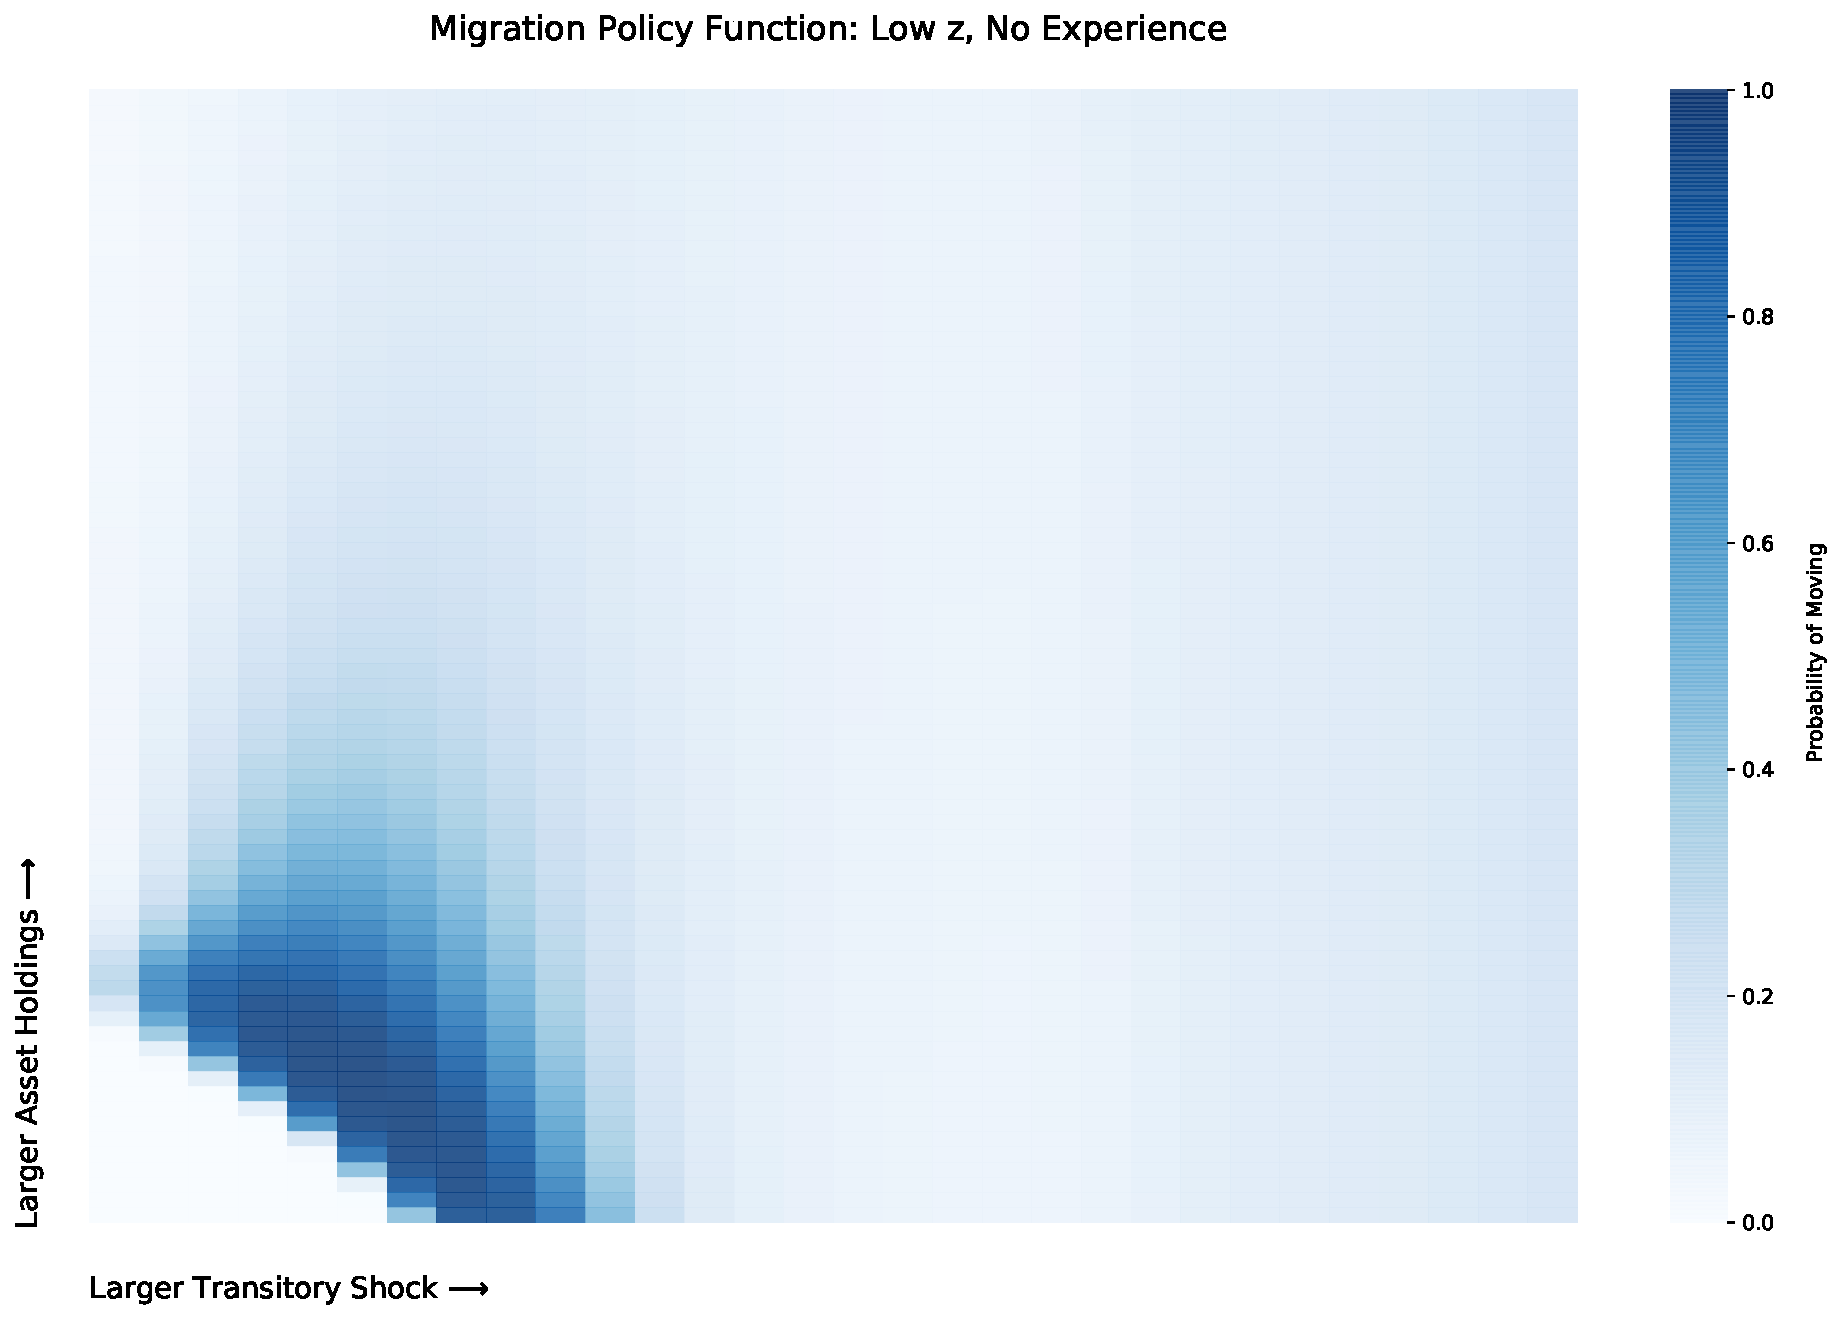
\includegraphics[scale=0.25,clip = true,]{../figures/migration_policy_low_z.pdf}}
          %\includegraphics[scale=0.56,clip = true,]{./Figures/fig2_lowz_notexp.eps}}
     \subfigure[Moderate $z$, not experienced \label{fig:modz}]{
          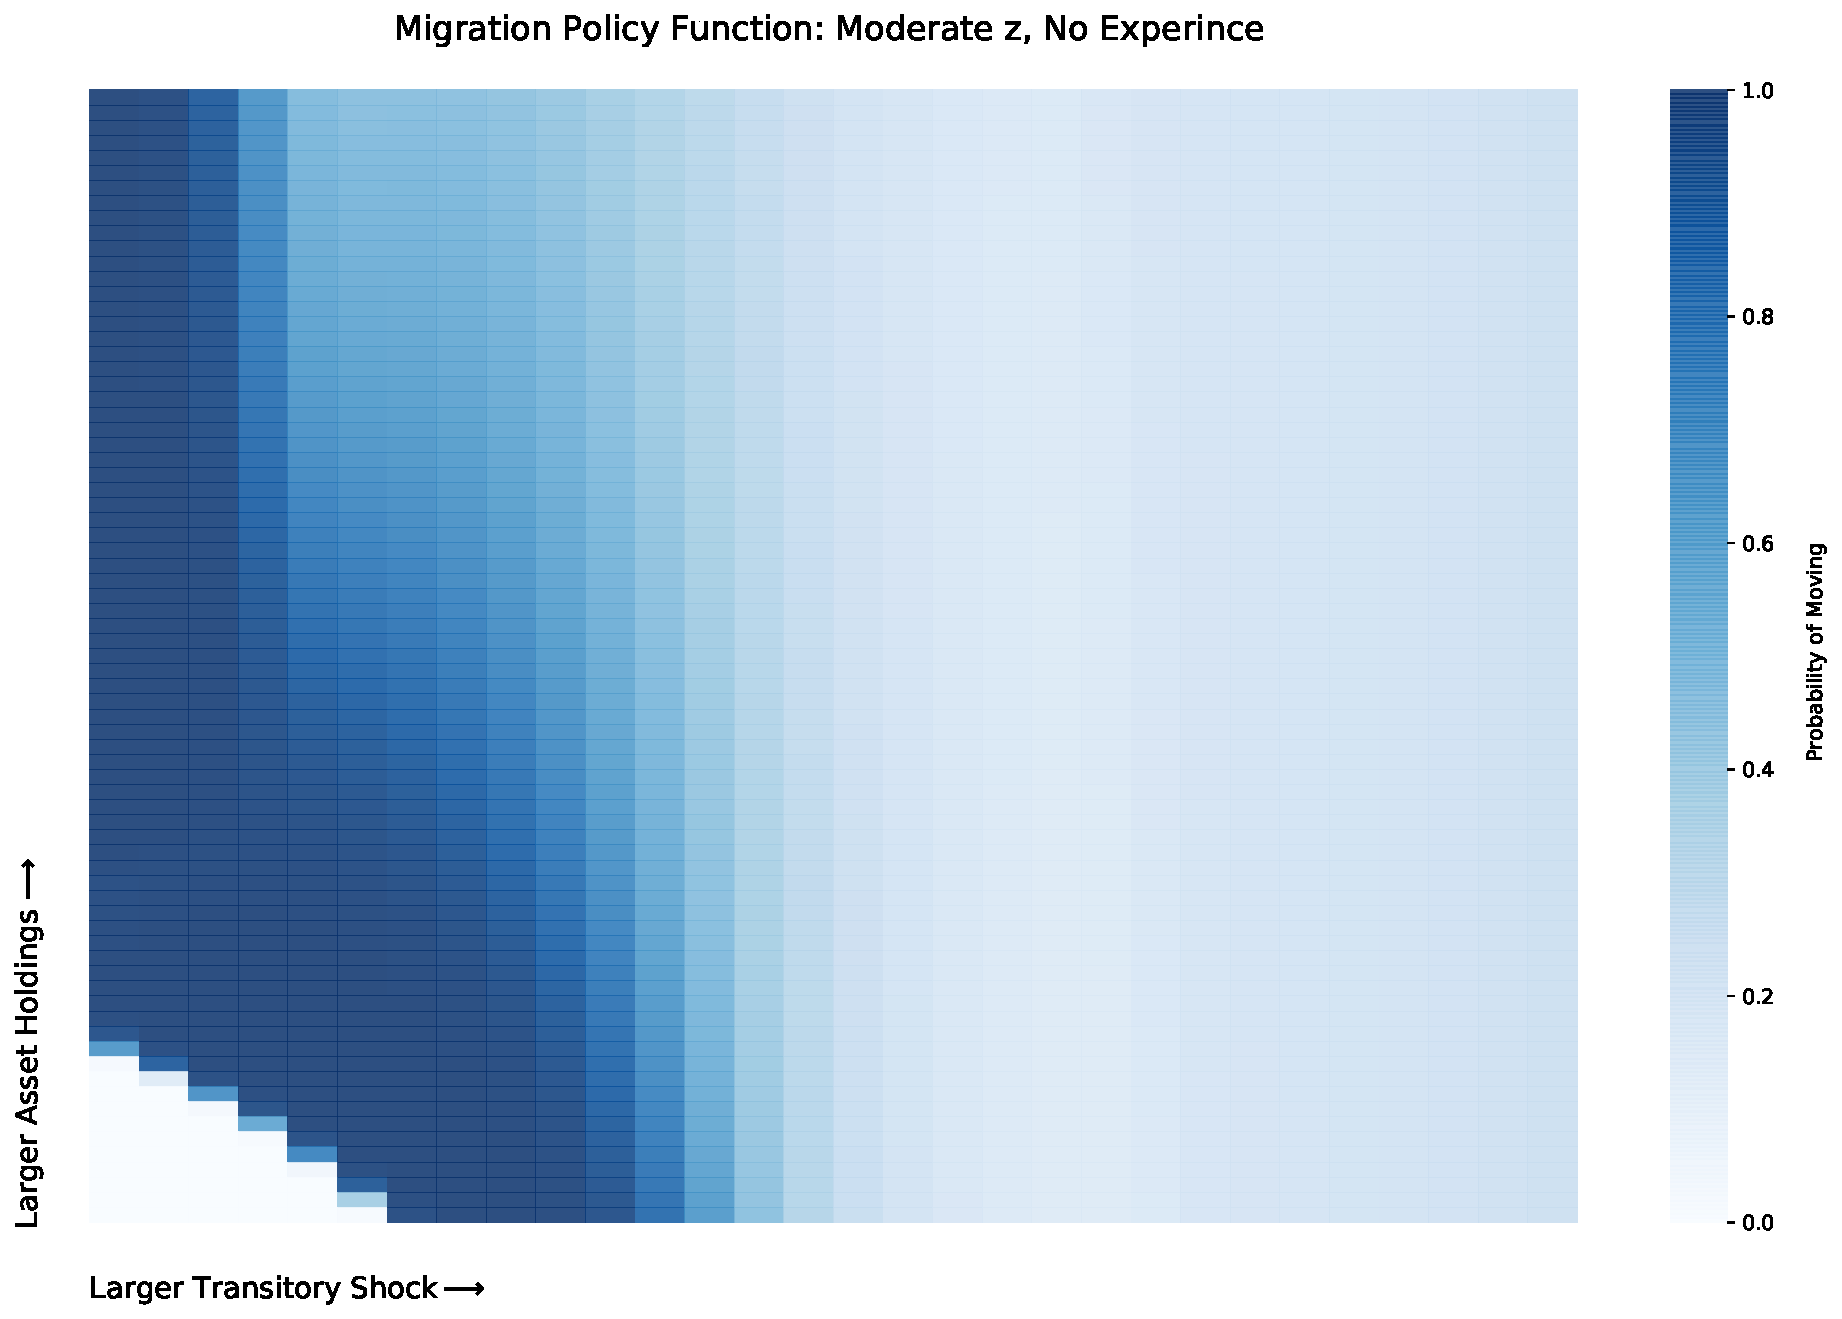
\includegraphics[scale=0.25,clip = true]{../figures/migration_policy_mod_z.pdf}}
          %\includegraphics[scale=0.56,clip = true]{./Figures/fig2_medz_notexp.eps}}
     \subfigure[Moderate $z$, experienced \label{fig:modz_expr}]{
          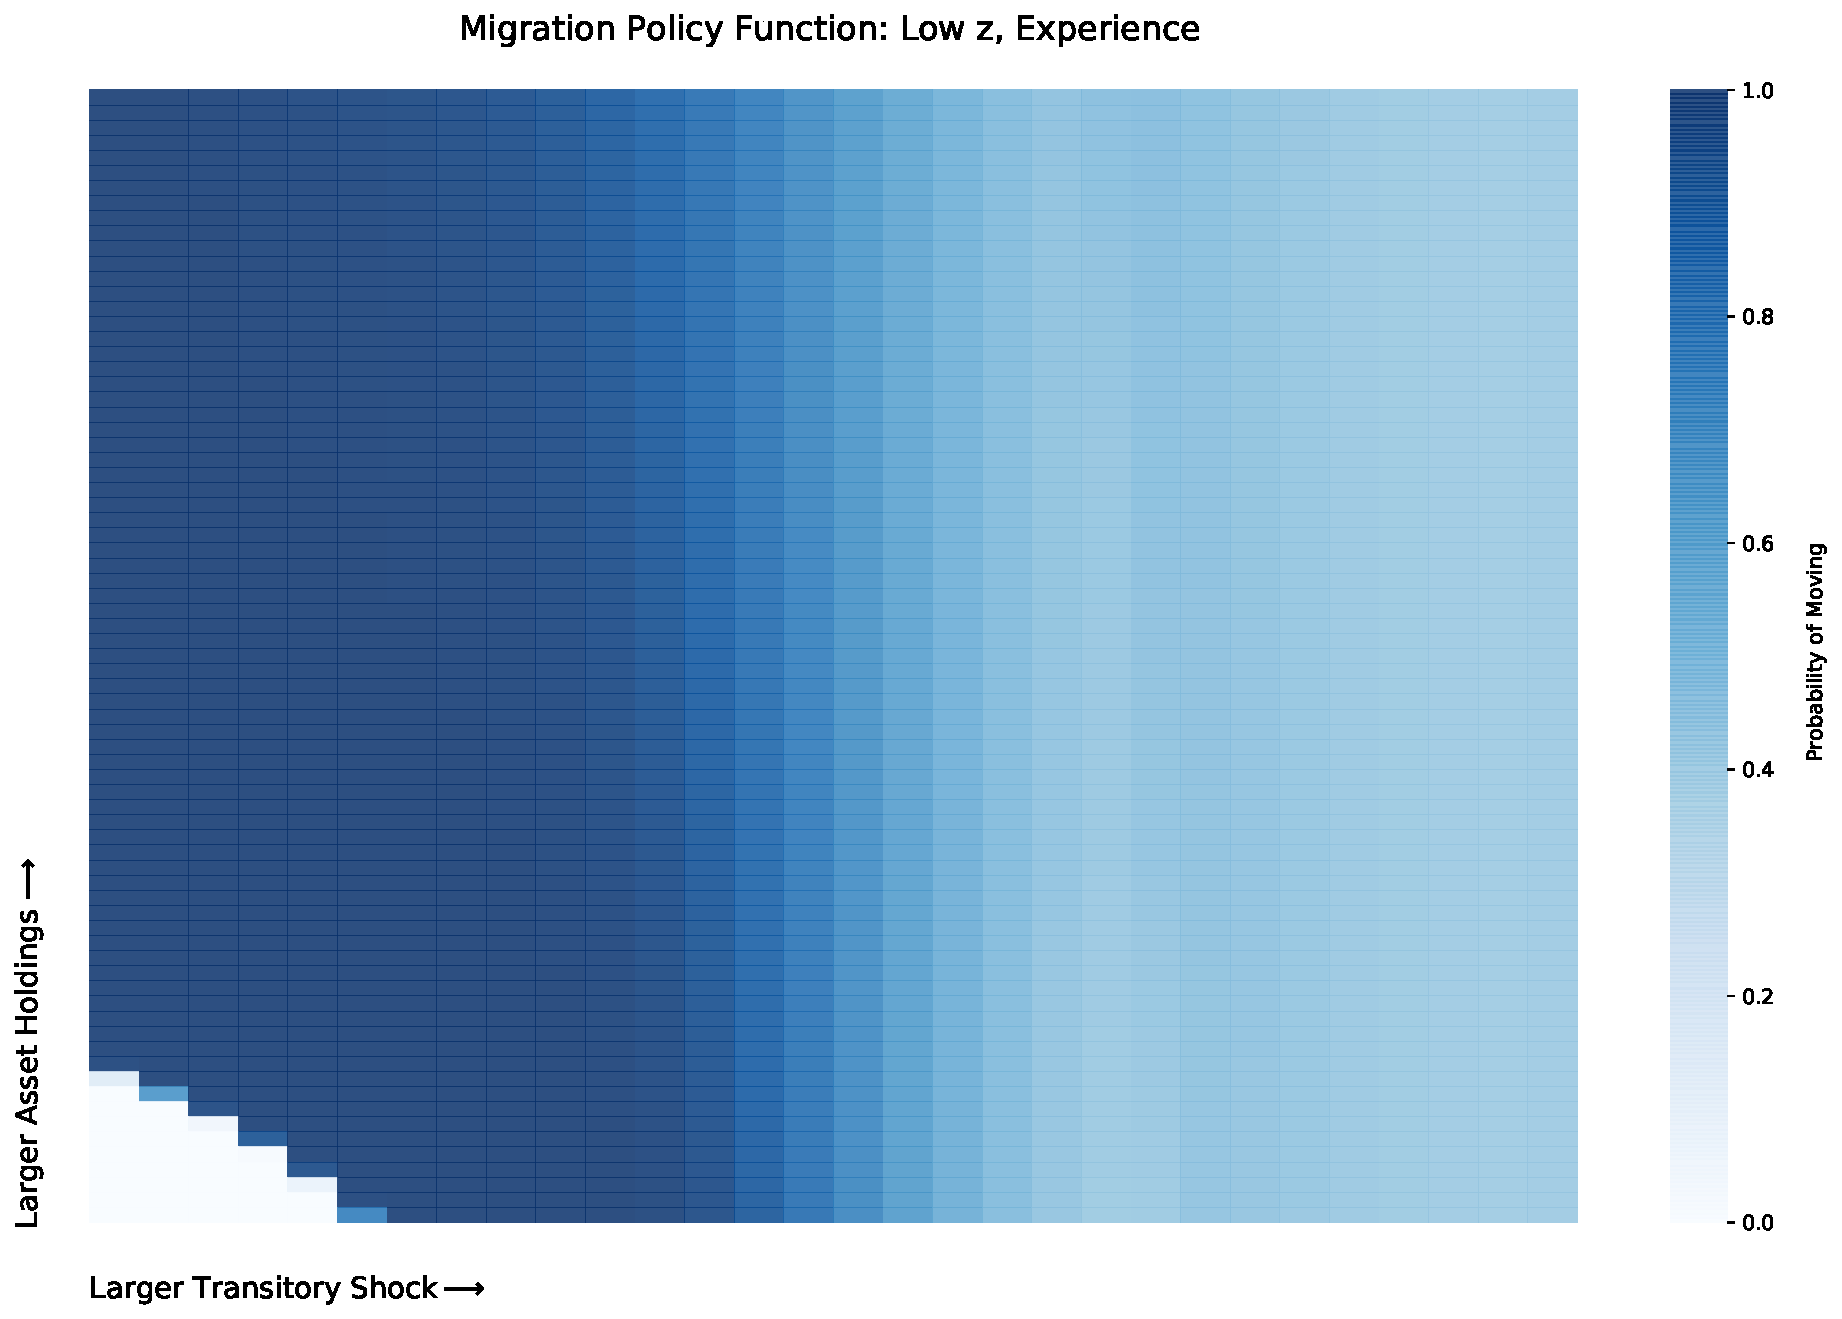
\includegraphics[scale=0.25,clip = true]{../figures/migration_policy_exp_z.pdf}}
         % \includegraphics[scale=0.56,clip = true]{./Figures/fig2_medz_exp.eps}}
\caption{Migration Probabilities for Select Household Types \label{fig:migration_policies}}
\end{figure}


%\end{sidewaysfigure}

\textbf{Higher urban productivity leads to more migration.} Panels (a) and (b) contrast the moving policy for low-$z$ households and moderate-$z$ households. The dark blue migration region in the southwest portion of the panels is larger for moderate-$z$ than for low-$z$ households. This means that those with a stronger comparative advantage are more likely to seasonally migrate to the urban area. Intuitively, the key data moment determining how many moderate-$z$ households there are, compared with the number of low-$z$ households, is the experimental migration response to the treatment.

This observation highlights an important implication about whom migration subsidies may affect. Households sort themselves into rural and urban areas largely on the basis of permanent comparative advantage. Thus, the set of households living in the rural area in any given period consists most likely of those with relatively low $z$ values. Households with higher $z$ are more likely to be in the city. As a policy, migration subsidies will be offered to those with low comparative advantage in the urban area.

\textbf{The disutility of the urban area is a important deterrent to migration.} Panels (b) and (c) of figure \ref{fig:migration_policies} contrast the moving policy for the same $z$ but different experience levels. Hence, these households face a disutility to migrating or not. The dark blue migration region is larger for the experienced household than for the inexperienced one. This illustrates the point that in the estimated model, we infer an important role for a non-monetary disutility of the urban area in shaping the migration choice.\footnote{To empirically investigate the source of the substantial migration disutility in our estimated model, we conducted some additional discrete-choice experiments on the same set of households used to estimate the model. We found evidence that potential migration opportunities involving poor housing conditions at destination were substantially less desirable in wage terms, all else equal. In particular, offering improved housing with a proper indoor latrine increases reported migration propensity by 17.4 percentage points. This effect size is equivalent to the effect of increasing migration wages by 21 percent. Thus, the lack of a good housing option after migrating, which is likely quite common for potential migrants in this setting, is one concrete example of the migration disutility in our model. See Appendix \ref{sec:discrete_choice} for a complete description of these discrete-choice experiments and our empirical findings.}

Several features of the data combine to push our model to infer a substantial non-monetary disutility of the urban area. At the most basic level, this is about the overall level of migration (not the experimental response which informs the distribution of ability). In the lean season, productivity falls by fifty percent, yet many do not migrate. One way for our model to accommodate this observation is to have a large disutility of migration.

The alternative explanation is that households simply cannot afford to migrate. The important observation is that whatever force prevents migration must be consistent with the consumption response and the pattern of selection implied by it. As we discuss next, in both the data and the model, migrants are negatively selected on assets and income. And a large disutility of migration (to get the overall migration flows correct) is consistent with the pattern of selection in the data; a credit constraint story is not.

\textbf{Households with low assets and low transitory shocks are more likely to migrate.} All three panels of Figure \ref{fig:migration_policies} highlight how households with low assets and low transitory shocks are more likely to migrate. This point is seen by noting that in all cases, the dark blue migration region always originates out of the southwest corner. If one's expectation is that credit constraints are the primary reason that households do not migrate, this may seem surprising. If migration costs are high and the credit constraint binds, then the migration region would originate from the northeast corner in Figure \ref{fig:migration_policies}, because this is where the constraint would be alleviated. In fact, credit constraints prevent migration for a very small part of our parameter space, seen as the white region in the very lower left corners of all three panels in the figure.

The key behind this result is the observation that the OLS coefficient from consumption regressed on migration is smaller than the IV (LATE) coefficient. Because OLS is smaller relative to IV, the implication is that migrants are \emph{negatively selected} on the determinants of consumption. In our model, a household's state variables are the determinants of its consumption | specifically, its transitory shock and asset holdings. Thus, the fact that the OLS coefficient is less than the IV coefficient pushes our model to accommodate the idea that households with low assets and low transitory shocks are more likely to migrate as in Figure \ref{fig:migration_policies}.

This push is achieved through a large $\bar u$ parameter (as described above), but it is also facilitated by the inference that rural area is very risky $\gamma <1$ and that households have a low return on their savings and hence difficulties self-insuring. That is, rural households generally prefer rural areas but sometimes find themselves in periods of low productivity and low assets, particularly in the lean season. Because self-insurance through savings is difficult, these households use seasonal migration as a form of insurance allowing them to temporarily raise their incomes and thus smooth their consumption over time. This latter observation is essentially a spatial analog to  \citet{PIJOANMAS2006}, in which households with low productivity or low assets increase their labor supply to self-insure.

This observation has an important implication for how migration subsidies may improve welfare in our model. They serve to channel resources toward the rural households that are unproductive and vulnerable owing to a lack of assets that can be used for self-insurance. In other words, the migration subsidy provides households an insurance opportunity to more easily supply their labor in the urban location.

\subsection{Non-Targeted Moments}

How does the model fare in predicting non-targeted moments? We answer this question by examining several features of the data: migration rates by initial consumption level, asset holdings by migration status, variances of consumption growth by migration status, and the migration effects of unconditional cash transfers.

We focus on these non-targeted moments for the following reasons. Looking at how migration rates vary by initial consumption level speaks to households' heterogeneous responses to the treatment.  Asset holdings by migration status tell us about the extent to which migration decisions are driven by buffer-stock savings strategies versus strategies in which migration serves as insurance when productivity and assets are low. The variance of consumption growth and the effects of unconditional transfers speak to the importance of potential spatial misallocation from credit constraints and migration risk, as in \citet{hato70} and the model of \citet{brch14}.

\textbf{Migration rates by initial consumption level.} Table \ref{ta:cal_parameters} reports the migration rates in the control group by the levels of consumption and assets. Panel A exhibits migration rates from the data, and panel B reports the value in the estimated model (which are not targeted). For simplicity, we consider consider consumption only above and below the median and assets above and below the 800 taka | approximately the size of the transfer.
As the table shows, migration rates are higher for people with lower consumption and asset levels. This suggests that migration in the data is, if anything, more likely for those with lower consumption levels to begin with. Our model gets this prediction largely correct.
\begin{table}[t]
\small
\setlength {\tabcolsep}{1.5mm}
\renewcommand{\arraystretch}{1.2}
\begin{center}
\vspace{0.3cm}

\textbf{\caption{Migration Rate by Asset and Consumption Level\label{ta:cal_parameters}}}

\vspace{0.3cm}

\begin{tabular}{c l | c c}
\multicolumn{4}{c}{\textbf{Panel A: Data}} \\
\hline\hline
 & & \multicolumn{2}c{Assets} \\
 & & $\leq$ 800 Taka & $>$ 800 Taka \\
\hline
\multirow{2}{*}{Consumption} & Below Median & 40\% &  29\% \\ %0.40 & 0.29 \\
 & Above Median & 36\% & 31\% \\  % 0.36 & 0.31 \\
\hline
\multicolumn{4}{c}{} \\
\multicolumn{4}{c}{\textbf{Panel B: Model}} \\
\hline\hline
 & & \multicolumn{2}c{Assets} \\
 & & $\leq$ 800 Taka & $>$ 800 Taka \\
\hline
\multirow{2}{*}{Consumption} & Below Median & 41\% &  28\% \\  %& 0.4077 &  0.2779 \\
 & Above Median & 41\% & 38\% \\ % & 0.4091 & 0.3788 \\
\hline
%\multicolumn{4}{l}{Savings split by whether the household could afford an 800 taka bus ticket} \\
%\multicolumn{4}{l}{Consumption split by median value} \\
\end{tabular}
\parbox[c]{4.25in}{%
{\footnotesize  \vspace{0.3cm} Note: The table reports the migration rates in the control group by consumption level and by level of assets, defined as cash plus bank account balances.  Panel A shows the migration rate in data. Panel B reports the rates from the estimated model.}
}

\end{center}
\end{table}

\textbf{Effects of unconditional transfers.} Table \ref{ta:bcm_comparison}, Panel B, reports the migration response in the data of an unconditional transfer, which was conducted along with the original migration experiments.  Households did respond positively to an unconditional transfer but to a much smaller extent than they did to the conditional transfers. However, the confidence interval is quite large and comfortably includes zero: the $p$-value of a test of the null hypothesis that the unconditional transfer has no effect is 0.24. In the model, the effect of an unconditional transfer is one percent higher migration. Thus, it is fair to say that the model predicts that an unconditional transfer has a smaller effect on migration than a conditional transfer, as in the data, and an effect that is small overall and within the confidence intervals of the model's prediction.

\textbf{Variances of consumption growth by migration status.} Table \ref{ta:cons_growth} lists the variance of log consumption growth for households that stay and those that migrate, in both the data and the model. In the data, the control group (upper panel) has log consumption growth variance of 0.15 for stayers and marginally higher variance, of 0.18 for those that migrate. The model is similar, with 0.18 for the stayers and a marginally higher at 0.19 for the migrants. The treatment group (lower panel) in the data is somewhat similar to the control group, and again the model matches the similar but marginally higher log consumption variance of the migrants.

\begin{table}[t]
\setlength {\tabcolsep}{4.99mm}
\renewcommand{\arraystretch}{1.2}
\small
\begin{center}
\textbf{\caption{Variance of Log Consumption Growth \label{ta:cons_growth}}}
 \vspace{0.3cm}
\begin{tabular}{l c c}
\hline
\hline
\multicolumn{3}{c}{Control Group}  \\
& Stay & Migrate \\
\hline
Data  &  0.15  &  0.18 \\
Model & 0.18 & 0.19\\
\hline
\end{tabular}
\begin{tabular}{l c c}
\hline
\hline
\multicolumn{3}{c}{Treatment Group}  \\
& Stay & Migrate \\
\hline
Data  &  0.16  &  0.19 \\
Model & 0.17 & 0.19 \\
\hline
\end{tabular}
\parbox[c]{5.0in}{\vspace{0.1cm}
{\footnotesize  Note: The table reports the variance of log consumption growth from before the lean season to afterwards. The left panel is for the control group, and the right panel is for the treatment group. The columns represent the set of households that stay (do not send a migrant) versus that of those that migrate (do send a migrant).}
}
\end{center}
\vspace{-0.3cm}
\end{table}
It is worth discussing how our model correctly predicts higher consumption growth variance for migrants compared with that of non-migrants, even though it features higher transitory shock variance in the rural area ($\gamma<1$). The reason is as follows. The model's prediction is that households with relatively low transitory shocks and asset levels do more temporary migration, all else equal. In the estimated model, these temporary migrants see large gains in income and hence consumption, since they are largely ``hand-to-mouth.'' This tends to increase consumption growth variance for migrants. In the aggregate, this force leads to larger consumption growth variance for migrants, even though migrants face lower income risk at the individual level.


\subsection{Identification}

In this subsection, we further illustrate how the experimental and cross-sectional moments help identify the parameters of the model. To do so, we start with the benchmark calibration and then compute the elasticity of each targeted moment to each parameter. Table \ref{ta:elast} reports these elasticities. For expositional purposes, we put in bold any elasticity greater than or equal to one in absolute value. It is useful to discuss the results in Table \ref{ta:elast} one parameter at a time, as well as the moments that are most sensitive to the change in parameters.

\begin{table}[!h]
%\footnotesize
\small
\setlength {\tabcolsep}{2mm}
\renewcommand{\arraystretch}{1.3}
\begin{center}
\caption{Elasticities of Targeted Moments to Parameters \label{ta:elast}}
\vspace{0.3cm}
\begin{tabular}{l c c c c c c c c c c}

\hline \hline

& $1/\theta$ & $A_u$ & $\rho$ & $\bar{u}$  & $\pi$ & $\lambda$ & $\gamma$ & $\sigma$  & $\sigma_\nu$ \\


\hline

Urban-rural wage gap & \textbf{1.6} & -0.2 & 0.5 & -0.0 & 0.1 & 0.0 & 0.2  & -0.5 & -0.1 \\

Percentage in rural & 0.9 & \textbf{-1.3} & 0.5 & -0.5 & -0.0 & 0.2 & 0.1 & -0.4 & 0.0 \\

Control: Percentage of rural with no liquid assets & -1.0 & 0.6 & \underline{\textbf{4.3}} & -1.0 & 0.1 & 0.1 & -0.2 & -1.2 & -0.0 \\

Control: Seasonal migrants & -3.5 & 1.8 & -0.3 & \textbf{-5.4} & \underline{-0.9} & \underline{1.8} & -0.8  & 0.2 & 0.1 \\

Treatment effect on seasonal migration & -1.6 & \textbf{2.1} & -0.8 & -1.3 & 0.4 & -0.4 & -0.1 & 1.0 & -0.1 \\

Treatment effect on seasonal migration, year 2 & -2.4 & \textbf{3.3} & -1.2 & 0.7 & -0.7 & 0.5 & 0.3 & 1.6 & -0.3 \\

Consumption increase of migrants (OLS) & \underline{4.8} & \underline{-3.5} & 4.3 & \underline{\textbf{8.2}} & 0.5 & -0.3 & \underline{2.9} & \underline{-3.0} & -0.3 \\

LATE - OLS & \textbf{-3.2} & 1.8 & 0.4 & -2.9 & -0.2 & 0.4 & -1.2 & -0.3 & -0.1 \\

Control: Probability of repeat migration & 0.0 & 0.2 & 0.2 & \textbf{-0.9} & -0.4 & 0.7 & 0.2 & -0.3 & \underline{-0.3} \\

\hline \hline

\end{tabular}
\parbox[c]{6.6in}{%
{\footnotesize  \vspace{0.5cm} Note: This table reports the elasticities of each targeted moment to each parameter, computed as the percent increase in each moment to a one percent increase in each parameter, starting from the estimated parameters of the model. The largest elasticity in absolute value in each row is printed in bold. The largest elasticity in absolute value in each column is underlined.}
}
\end{center}
\end{table}


%Control: Variance of log consumption growth in rural            & 0.19              & 0.19              & 0.19              \\
%Control: Percent of rural households with no liquid assets      & \phantom{0.}47    & \phantom{0.}47    & \phantom{0.}48   \\
%Control: Seasonal migrants                                      & \phantom{0.}36    & \phantom{0.}36    & \phantom{0.}38   \\
%Control: Consumption increase of migrants (OLS)                 & \phantom{0.}10    & \phantom{0.}10    & \phantom{0.}13   \\
%Treatment: Seasonal migration relative to control               & \phantom{0.}22    & \phantom{0.}21    & \phantom{0.}21   \\
%Treatment: Seasonal migration relative to control in year 2     & \phantom{0.}9     & \phantom{0.}5     & \phantom{0.}06   \\
%Treatment: Cons of induced migrants relative to control (LATE)  & \phantom{0.}30    & \phantom{0.}29    & \phantom{0.}26   \\
%Control: Probability of repeat migration                        & \phantom{0.}68    & \phantom{0.}71    & \phantom{0.}69   \\
%\hline
%Urban-Rural wage gap                                            & 1.89              & 1.89              & 1.90             \\
%Percent in rural                                                & \phantom{0.}61    & \phantom{0.}60    & \phantom{0.}60   \\
%Variance of log wages in urban                                  & 0.56              & 0.56              & 0.56              \\


For expositional purposes, we highlight in bold type the largest elasticity (in absolute value) in each row so as to illustrate which parameters have the most substantial impact on each moment. Similarly, we underline the largest elasticity (in absolute value) in each column to show which moment is most affected by each parameter change. We focus on the nine parameters for which identification is not obvious. The measurement error terms are informative only about the variances of income and consumption growth, so we omit those from the table. For expositional purposes we also focus on the difference between the LATE of migration on consumption and the OLS effect, since we find the difference more informative about the added value of the LATE coefficient relative to the OLS effect in identifying the model.

Starting with the moments, we find that the wage gap is most responsive to $\theta$. The idea is that when $1/\theta$ is larger, there is more variance in permanent productivity, which increases the importance of sorting in driving wages up in urban areas relative to rural ones. The rural population share responds the most to changes in $A_u,$ indicating that the level of urban productivity is the most important determinant in the model of the relative population size there. The fraction of rural households without any assets is most sensitive to $\rho.$ The intuition is that when the shock process is more autocorrelated, more households eventually find themselves with low asset holdings after a bad shock.

The seasonal migration rate in the control group is most sensitive to $\bar u$, indicating that migration costs are the most important determinant of seasonal migration among those not offered incentives. The same is true of the OLS coefficient of migration on consumption and the probability of repeat migration in the control group. In contrast, the treatment effects on migration are most sensitive to $A_u$, which obviously plays an important role in governing the benefits of seasonal migration. The difference between the LATE of migration on consumption and the OLS effect is most affected by $\theta.$ This indicates that sorting patterns in the model are a key determinant of the consumption increases after being induced to migrate, relative to an observational difference in consumption levels between migrants and non-migrants. In other words, the LATE coefficient helps identify the extent to which induced migrants are selected differently than migrants who move out of their own volition.

An additional set of insights emerges from Table \ref{ta:elast} from looking down the columns and asking which moment is most affected by each parameter. The parameter $\theta$, governing the variance of permanent urban productivity, has the largest effect on the OLS coefficient. This parameter also has a large effect on the LATE of migration on consumption. The implication is that greater scope for sorting on permanent ability implies higher returns to migration but smaller gaps between the returns of induced and non-induced migrants. The parameter $A_u$ also has the largest impact on the OLS return to consumption, since it determines the productivity advantage of working in the urban area.

The autocorrelation of transitory shocks, $\rho$, has the largest impact on the percentage of rural households that have no assets, again signaling how levels of asset holdings are identified largely by this autocorrelation term. The migration cost $\bar u$ has the largest impact on the OLS effect of migration on consumption, though it also has a large effect on the seasonal migration rate in the control group and, to a lesser extent, the difference between the LATE and OLS effects of migration. This highlights how the extent of and returns to seasonal migration help discipline the migration cost in the model.

The probabilities of remaining experienced and inexperienced, $\pi$ and $\lambda$, have the largest impacts on the seasonal migration rates in the control group. The reason is that in the model, individuals are a lot more likely to migrate when they are experienced. The higher the probability of remaining experienced, and the lower the probability of remaining inexperienced, the greater is the number of control households with experience in equilibrium, and the higher is the seasonal migration rate. These two parameters also impact repeat migration rates, both in the treatment and control groups, though interestingly these are not the most affected moments.

The parameters $\gamma$ and $\sigma$ have the largest impact on the OLS return to migration, and $\gamma$ also has a sizable impact on the difference between the LATE and OLS coefficients. The link to the OLS return to migration implies that $\gamma$ is being identified in part from the extent to which migrants are positively or negatively selected on transitory shocks. When $\gamma$ is smaller, households induced to migrate are more likely to be those with lower transitory shocks and few asset holdings. If these households migrate, therefore, they are more likely to be those with the relatively lowest productivity draws in the urban areas. This, in turn, leads to a lower OLS coefficient of consumption migration, since those deciding to migrate have relatively lower consumption levels.

The parameter $\sigma_{\nu}$, which governs the variance of the migration taste shocks, has a modest impact on most of the moments. The largest effect is on the probability of repeat migration in the control group, followed by the treatment effect on repeat migration. The intuition is that when taste shocks tend to be larger in absolute value, they play a more substantial role in determining migration decisions in each period.

Another way of illustrating how the model is identified comes from re-estimating the model under specific parameter restrictions. This approach prevents the model from matching the targeted moments as well as the benchmark estimation, since the model has fewer degrees of freedom once parameters are restricted ex-ante. The value comes from seeing exactly how the model fails once particular parameters are restricted.
\begin{table}[t]
\small
\setlength {\tabcolsep}{1.0mm}
\renewcommand{\arraystretch}{1.2}
\centering
\textbf{\caption{Model Moments When Model Is Restimated under Parameter Restrictions \label{ta:alt_est_2}}}
\vspace{0.3cm}

\begin{tabular}{c c c c c c c}
\multicolumn{6}{c}{\textbf{\normalsize }}\\
\hline
\hline
Moments & Data & Baseline & $\theta = \infty$ & $\bar u = 1$ & $\lambda = 0$  & $\gamma = 1$ \\
\textbf{Control}\\
Migration                                                        & 36    & 32    & 48 & 29  & 37 &  26 \\
Repeat Migration, year 2                               & 25    & 25    & 31 & 27  & 25   &  25 \\
Repeat Migration, year 4                               & 16    & 18    & 16 & 25  & 18   &  23 \\
Consumption gain, migrants (OLS)               & 10    & 10    & 51 & 2 & 10 & 20 \\
\hline
\textbf{Experiment}\\
Migration                                   & 22    & 20    & 31 & 10 & 16 & 18 \\
Migration, year 2                           & 9     & 6     & 0 & 0 & 0 & 6 \\
Consumption gain, induced migrants (LATE)   & 30    & 30    & 20 & 6 & 30 & 30 \\
\hline
\textbf{Aggregate}\\
Urban-Rural wage gap                                    & 1.80  & 1.80 & 1.80 & 1.80 & 1.80 &  1.80 \\
Percentage in rural                                        & 63 & 63 & 57  & 89  & 92 & 58 \\
\hline

\end{tabular}

\parbox[c]{6.75in}{\vspace{0.1cm}
{\footnotesize  Note: The table reports the values of eight moments of the model when the model is re-estimated under restrictions on model parameters. The first column contains the moments in the data, and the second contains the moments from the estimated model. The remaining columns present the model's moments when estimated to match the same moments but assuming that one particular parameter is restricted ex-ante. Specifically, these columns focus on the cases when $\theta = \infty$, meaning no permanent worker heterogeneity; when $\bar u = 1$, meaning no migration disutility; when  $\lambda = 0$, meaning no chance of retaining migration experience; and when $\gamma = 1$, meaning transitory shocks are equally volatile in both regions.}}
\end{table}

Table \ref{ta:alt_est_2} presents the best fit of the targeted moments under four specific parameter restrictions. The first two columns reproduce the targeted moments from the data and the estimates from the baseline model. The third column illustrates the model's best fit taking $\theta \rightarrow \infty$ as a numerical limit, implying that heterogeneity across workers is negligible. In this case the model struggles to match the migration rate of 36 percent in the control group, predicting 48 percent instead. The model also over-predicts repeat migration patterns somewhat. The main failure of the model under this restriction is that the OLS return to consumption is far too high at 51 percent, and the LATE of migration on consumption is too low at 20 percent. This is consistent with the discussions above about Table \ref{ta:elast}, which highlighted migration rates in the control group and returns to migration as helping identify the extent of worker heterogeneity in the model.

The fourth column of Table \ref{ta:alt_est_2} reports the best fit of the model when $\bar u = 1$ | that is, when migration disutility is shut off. This version of the model under-predicts migration rates in the control group but over-estimates them in subsequent years. Without disutility of migration, in other words, the model cannot match the dynamics of migration patterns. The OLS and LATE effects of migration on consumption are also far too low. This suggests that the model cannot support large gains from migration in equilibrium without large migration costs. The returns to migration, in other words, play a key role in identifying the model's migration cost.

The next column explores the model's fit when $\lambda = 0$, meaning that no individual can retain migration experience. In this case, migration rates in the control group are not too far off, including repeat migration rates in years 2 and 4. Yet the treatment effect on migration is too low, and there is no repeat migration at all from the experiment. This highlights the fairly direct way in which repeat migration after induced migration informs the model's parameters about the dynamics of migration experience.

The last column of Table \ref{ta:alt_est_2} explores the case when $\gamma$ is restricted to equal one, meaning that transitory shocks are equally volatile in rural and urban areas for potential migrants. Migration rates in this version of the model are too low, and repeat migration is again too high. The OLS return to migration is also about twice as high as in the data, meaning that the OLS and LATE coefficients are counterfactually close to each other. The model's inability to match these two measured returns to migration signals their importance in identifying the parameter $\gamma$ in the model, which is paralleled to some extent in Table \ref{ta:elast}.


%%%%%%%%%%%%%%%%%%%%%%%%%%%%%%%%%%%%%%%%%%%%%%%%%%%%%%%%%%%%%%%%%%%%%%
%%%%%%%%%%%%%%%%%%%         Comparions to Bryan et al (2014) Model              %%%%%%%%%%%%%%%%%%%%%%%%
%%%%%%%%%%%%%%%%%%%%%%%%%%%%%%%%%%%%%%%%%%%%%%%%%%%%%%%%%%%%%%%%%%%%%%

\subsection{Comparison to Model of Bryan et al. (2014) \label{sec:bcm_lmw}}

We now compare our model with the one proposed by \citet{brch14} and show that their model is quantitatively inconsistent with the experimental evidence. As a result, it leads to an inaccurate interpretation of the experiment. To recap, the model of \citet{brch14} has three main features: migration risk, a credit constraint that prevents households from borrowing to migrate, and individual learning about urban productivity. The model starts from pre-specified (i.e., non-equilibrium) initial conditions and offers a conditional migration transfer to all model households in the rural area. Rural households differ in permanent urban ability and their stock of assets, which they can accumulate through buffer stock savings. In contrast to our model, there is no disutility of migration, and there are no temporary productivity shocks. Learning in their model is permanent: no worker knows his or her productivity in the urban area until after migrating, and then the worker learns it forever.

To compare their model's prediction with the data, we assume a common CRRA parameter of two, which is the same value used in the current model and in the middle of the range of values explored by \citet{brch14}. We compare our model's predictions with the data and their model, starting from their preferred initial conditions. A key difference between the two models' predictions is in the constraints that hold back migration, which determine how migrants are selected in equilibrium. In the model of \citet{brch14}, many households would like to migrate, but they lack the credit or savings to do so. Their decision rule for migration is to migrate once disposable income reaches a certain threshold. A migration subsidy in that model induces migration by pushing up households over the threshold. In contrast, in our model, households wait until their prospects in the rural area are sufficiently bad for them to migrate, which means that households with lower income and asset levels migrate.

\begin{table}[t!]
\small
\setlength{\tabcolsep}{10mm}
\renewcommand{\arraystretch}{1.2}
\begin{center}
\textbf{\normalsize{\caption{Comparison to Model of Bryan et al. (2014)  \label{ta:bcm_comparison}}}}
%\scriptsize
\setlength{\tabcolsep}{9mm}
\vspace{0.4cm}
\begin{tabular}{l c c}
\multicolumn{3}{c}{\textbf{Panel A: Effect of Migration on Consumption }}\\
\hline
\hline
 & \;\;\; OLS \;\;\; & \;\;\; IV (LATE) \;\;\;  \\
%\hline
Data & 10 & 30 \\
Model & 10  & 29  \\
Model of Bryan et al. (2014) & 57  & 52  \\
\hline
\end{tabular}

\vspace{0.4cm}

\begin{tabular}{l c c}
\multicolumn{3}{c}{\textbf{Panel B: Effects of an Unconditional Transfer on Migration }}\\
\hline
\hline
 & \;\; Control \;\; & \;\; Treatment \;\;  \\
%\hline
Data & 34  & 44 \\
Model & 36  & 37  \\
Model of Bryan et al. (2014) & 66 & 88 \\
\hline
\hline
\end{tabular}

\vspace{0.3cm}
\parbox[c]{5.8in}{%
{\footnotesize
Note: This table reports moments of the experimental data and the predictions for the same moments in the current model and the model of Bryan et al. (2014). Panel A reports the values of the OLS and IV (LATE) returns to migration on consumption per capita, expressed in percentage points. Panel B reports the migration responses to an unconditional cash transfer in the control and treatment villages.
}
}
\end{center}
\end{table}

As one way to illustrate this, Panel A of Table \ref{ta:bcm_comparison} reports the effect of migration on consumption in the data and models, measured two different ways. The first way is the simple OLS coefficient from a regression of consumption on whether the household sent a seasonal migrant. The second is the LATE of migration on consumption, measured using an IV regression with migration instrumented using assignment to the treatment group. As the first two rows of Panel A show, the OLS coefficient on migration is substantially lower than the IV coefficient both in the data and in the current model.  As we discussed above, getting an OLS coefficinet smaller than the IV coefficient is a key determinant of whether model households that choose to migrate are negatively or positively selected on income and assets. Bryan et al.'s model has a counterfactually high coefficient: 57 percent, compared with 10 percent in the data.
Its IV coefficient is also too high: 52 percent, compared with 30 percent in the data. Perhaps most importantly, its OLS coefficient is counterfactually higher than the IV coefficient.

%%\begin{figure}[t!]
%%     \centering
%%\textbf{     \caption{Migration Rate by Consumption Quintile}}
%%\label{fig:migration_by_cons}
%%     \subfigure[\textbf{Data}]{
%%          \includegraphics[scale=0.63]{./Figures/fig4_data_nov_2019_revision.eps}}
%%     \subfigure[\textbf{Baseline Model}] {
%%          \includegraphics[scale=0.63]{./Figures//fig4_LMW_nov_2019_revision.eps}
%%           %\includegraphics[scale=0.7]{./Figures//quantile_cc_bcm.eps}
%%           }
%%                \subfigure[\textbf{Model of Bryan et al (2014)}]{
%%          %\includegraphics[scale=0.7]{./Figures//fig4_LMW.eps}
%%           \includegraphics[scale=0.63]{./Figures//quantile_cc_bcm-DL.eps}}
%%\end{figure}
%%
%%Figure \ref{fig:migration_by_cons} provides an alternative way to see how migration is determined in the two models and in the data. All three subfigures plot migration rates by consumption quintile in the control group (light blue), the treatment group (medium blue), and the simple difference between the treatment and control groups (dark blue). Panel (a) represents the data, panel (b) the predictions of the model and panel (c) the predictions of the model of Bryan et al. In the data, one can see that migration rates are higher in the treatment than in the control group across all consumption quintiles. The differences are similar across quintiles, and somewhat larger in the lowest quintile.
%%
%%Subfigures (b) and (c) of Figure \ref{fig:migration_by_cons} show the stark differences between the predictions of two models. In the current model, migration rates are higher in the treatment than in the control across all five quintiles, and somewhat larger in the lowest quintile. This parallels the data closely. In the model of Bryan et al, migration rates are identical in the highest two quintiles, and counterfactually high at one-hundred percent. Thus, it is those with the highest consumption levels that migrate, as these households are following a simple rule of migration once assets are sufficiently high (at which point consumption levels are high as well). The reason the treatment has an effect for the other quintiles is that the migration subsidy pushes other households up over the threshold. However, as one can plainly see in panel (a) of Figure \ref{fig:migration_by_cons}, this is not an empirically accurate depiction of how households make migration decisions in the data.
%%
%%Panel B of Table \ref{ta:bcm_comparison} reports the average asset holdings of migrants and non-migrants from the control group of the experimental data, and the corresponding predictions from the two models. Asset holdings are expressed as a ratio of average monthly consumption (across the entire control group). In the data, migrants have somewhat lower reported asset holdings (0.7 months of average consumption) than non-migrants (0.8 months). The same is true in the current model, with 0.4 months of assets for migrants compared to 0.5 months for non-migrants. Recall that these moments are not targeted in our estimation. The model of Bryan et al predicts that migrants have far higher asset levels (1.1 months) than non-migrants (0.5 months). This highlights yet again the counterfactual nature of migration decisions in the Bryan et al model, in which households migrate once they have sufficiently large buffer stocks of assets.

Another way of comparing the migration incentives in the two models is by considering the effects of an \emph{unconditional} transfer that \citet{brch14} conducted as a component of the original experiment, on a smaller subset of villages. Panel B of Table \ref{ta:bcm_comparison} reports the effects of this unconditional transfer in the data and in the two models. The top row reports the seasonal migration rates in the control and treatment groups, their simple difference, and the standard error of the difference. In the data, the migration rates were 34 percent in the control villages and 44 percent in the villages with the unconditional transfers, for a difference of 10  percentage points. The standard error of this difference is 6.5 percent, however, and the $p$-value is 0.24, meaning that this estimated effect is statistically insignificantly different from zero at any conventional significance level.

The bottom three rows of Panel C report the predicted effects of an unconditional transfer in the current model and the model of Bryan et al.  Our model predicts that unconditional transfers induce a negligible increase in migration of around one percent. Again, this moment is not targeted. The model of Bryan et al. predicts a counterfactually large increase in migration rates of 22 percentage points. This substantial increase again reflects the constraints on migration in that model | namely, that households cannot save or borrow | and the migration decisions that involve migration once assets are sufficiently high. The unconditional transfer helps the agents in that model get above the threshold asset level needed to make migration worthwhile.\footnote{The model of Bryan et al. also emphasizes subsistence consumption and permanent learning about migration ability, though in hindsight, neither of these features seems central to the interpretation of the experimental evidence in question. As we show in Appendix Tables \ref{ta:migration_model_data}, the predictions of the model of Bryan et al. are similarly counterfactual with and without subsistence constraints. Furthermore, the interpretation of the experimental evidence reached by the current model is not substantially changed once we add subsistence constraints (see Appendix Tables \ref{ta:data_model_subsistence} and \ref{ta:welfare_subsistence}). As for permanent learning about migration ability, in Appendix Table \ref{ta:repeat_migration_model_data} we show that the model of Bryan et al. makes counterfactually high predications for repeat migration rates.}


\section{The Welfare Effects of Conditional Migration Subsidies\label{sec:welfare}}

Given that the model does well in matching the salient features of the data, we feel confident in using it to measure the welfare implications of encouraging rural-urban migration through migration subsidies. To do so, we compute welfare as the consumption-equivalent metric used in macroeconomics since \citet{luca85} and extensively thereafter. This welfare metric computes the percent increase in consumption, $p$, that makes the household indifferent between a $p$-percent consumption increase in perpetuity and being offered the conditional migration subsidy.

\subsection{One-Time Migration Subsidies in Partial Equilibrium}

We begin by computing the welfare gains of a one-time migration subsidy for rural households with low assets. We treat the migration subsidies as unanticipated, available only to the bottom half of the rural asset distribution, and in partial equilibrium, meaning that we hold rural wages fixed and without financing the transfers. Instead, as in the experiments, the funding for the transfers comes from outside the economy. As a frame of reference, we also compute the welfare gains of a one-time unconditional transfer to this same population. To compare apples to apples, we choose the size of the transfers to each household so that the total cost of the transfers equals the total cost of the migration subsidies.

\begin{table}[h]
\small
\setlength {\tabcolsep}{1.95mm}
\renewcommand{\arraystretch}{1.4}
\begin{center}
\textbf{\caption{Welfare Effects of One-Time Migration Subsidies}\label{ta:welfare_quintile}}

\vspace{0.3cm}

\begin{tabular}{c c c c c c c c c c c}
\hline
\hline
& & \multicolumn{2}{c}{Migration Subsidy} && \multicolumn{2}{c}{Migration Subsidy} && \multicolumn{2}{c}{Unconditional Transfer} \\
& & \multicolumn{2}{c}{Migration Endogenous} && \multicolumn{2}{c}{Migration Policy Fixed} && \multicolumn{2}{c}{Migration Endogenous}\\
\cmidrule(lr){3-4} \cmidrule(lr){5-7}     \cmidrule(lr){8-10}
& & \small Welfare  &\small Migr. Rate  && \small  Welfare  &\small Migr. Rate && \small  Welfare  &\small Migr. Rate \\
\multirow{5}{*}{\rotatebox{90}{\small Income Quintile}}                 & 1 & 1.17  & 85 && 0.77 & 48 && 1.05 & 45 \\
                                                       				    & 2 & 0.45  & 63 && 0.31 & 38 && 0.56 & 37 \\
                                                        				& 3 & 0.29  & 52 && 0.20 & 34 && 0.40 & 33 \\
                                                       				    & 4 & 0.20  & 46 && 0.15 & 31 && 0.32 & 31 \\
                                                      				    & 5 & 0.12  & 40 && 0.10 & 31 && 0.20 & 31 \\
\hline
\multicolumn{2}{l}{\small \underline{Average}}      &  & &&  & &&   &  \\
\multicolumn{2}{l}{\small Rural \& Low Assets}          &0.44  & 57 && 0.30 & 36 &&  0.51 &  35 \\
\multicolumn{2}{l}{\small All Rural}                    &0.22  & 41 && 0.15 & 31 &&  0.25 &  30 \\
\hline
\end{tabular}

\parbox[c]{6.8in}{%
{\footnotesize  \vspace{0.1cm} Note: The table reports the lifetime consumption-equivalent welfare gains to rural assets with low assets from one-time conditional migration subsidies and from a one-time unconditional transfer. The rows are for different income quintiles of the rural households eligible for the subsidy, which are those in the bottom half of the rural asset distribution, with 1 being the poorest quintile and 5 being the richest. The first column reports the results of a one-time migration subsidy when the migration policies are held fixed for every agent. The second column is the same but shows the results when migration responds endogenously. The third column reports the results of a one-time unconditional transfer costing the same total amount as the migration subsidies in the second column. All three experiments are in partial equilibrium, meaning that the rural wage is held fixed and the subsidies or transfers are not financed in equilibrium.}
}
\end{center}
\end{table}


Table \ref{ta:welfare_quintile} reports the welfare gains from the migration subsidy and unconditional transfer. For expositional purposes, we report the average welfare gain and seasonal migration rate by income quintile among rural households eligible for the subsidy (with one being the lowest). The first two columns of Table \ref{ta:welfare_quintile} focus on migration subsidies with endogenous migration responses, which represent the migration subsidies described in the field experiments of Section 2. Several features of these two columns are worth noting. First, the welfare gains for the one-time migration subsidy are modest on average, at 0.44 percent consumption equivalents. Second, gains are higher for the poorer quintiles and reach as high as 1.17 percent consumption equivalents for the poorest quintile. Third, migration rates are higher for the poorer quintiles, reaching as high as 85 percent for the poorest quintile. The average migration rate of 57 percent corresponds to the migration rate of the treatment group of the original migration experiment.

The middle two columns of Table \ref{ta:welfare_quintile} report the welfare effects of the conditional migration transfers where we make the transfers to all households willing to migrate given the transfer but counterfactually hold the migration polices of each household fixed at pre-transfer levels. The purpose of this exercise is to illustrate how many of the gains occur just from making the transfers to the households willing to undergo the ordeal of seasonal migration in order to obtain the transfer. The welfare gains from this exercise are 0.30 consumption equivalents on average and rise up to 0.77 consumption equivalents for the poorest quintile. This implies that many of the welfare gains from the migration subsidies | around two thirds of them | arise just from making the transfers to the households willing to take them. Notice that the actual migration rates in this exercise are identical to the equilibrium without transfers, highlighting that none of the welfare gains here arise from actually migrating.

The last two columns report the welfare effects of making unconditional transfers to the same set of households, where the total amount of the transfers equals the total cost of the migration subsidies in the previous two exercises. Notice that this implies a smaller transfer to each household, since every eligible household gets the unconditional transfer, whereas only 57 percent of eligible households take up the migration subsidy. Overall, the unconditional transfers lead to modestly higher average welfare gains than the migration subsidies, at 0.51 percent consumption equivalents. The poorest households gain less, since they get a smaller transfer, and the richest gain more, signaling that the transfers are less precisely targeted to needier households. Interestingly, migration rates are far lower under the unconditional transfers, meaning that few eligible households actually want to migrate when given the choice not to do so. This is consistent with the evidence (discussed in Section \ref{sec:bcm_lmw}) on how an unconditional transfer had a modest effect on migration.

Revisiting figure \ref{fig:migration_policies} allows one to get some additional insight into how the welfare gains arise in the model. Panel (a) of the figure shows the policy functions for a household with a low level of $z$ and no migration experience, in the control group. The policy functions for the treatment group are not depicted (for expositional purposes) but would expand the migration regions up and to the right. In the figure, household (i) is inframarginal and will make a temporary move whether or not it is offered a conditional migration transfer. Household (ii) is on the margin and is induced to migrate by a conditional transfer, but it would otherwise stay in the rural area. What households (i) and (ii) have in common is that they are willing to go through with the ordeal of migration since marginal utility of consumption is so high for them. Household (iii) will not migrate even when offered a transfer. Given the high level of assets and the high shock, this household prefers the rural area even with the transfer.

Who gains the most from the conditional migration transfers? Perhaps surprisingly, it is household (i), the inframarginal household. This household has low levels of assets and a bad shock, so it has a very low level of consumption. Marginal utility is relatively high for this household, so the transfer leads to a relatively large increase in its welfare. Household (ii) also gains a lot, but by somewhat less than household (i), since household (ii) has a higher level of consumption before the transfer. It is true that this household changed its behavior as a result of the experiment, but that is not the key driver of welfare gains. Rather, it is the channeling of funds to the vulnerable households, which are the only ones willing to go through with the ordeal of migration. Household (iii) doesn't take up the conditional transfer, and so the intervention does not change its welfare at all.

\subsection{Permanent Migration Subsidies in General Equilibrium}

We now consider the welfare gains from permanently offering migration subsidies to rural households with low assets, using the same asset availability criteria as for the temporary transfers above. We simulate offering these policies in general equilibrium | meaning that we allow rural wages and population shares to adjust | and financing the transfers through taxation of labor income on all households. We report the welfare gains on average for four subgroups of the population: rural households with low assets (i.e., those eligible for the subsidies), all rural households, all urban households, and all households.

Table \ref{ta:welfare_permanent} reports the welfare gains for these population subgroups and other key statistics. We first report the welfare gains of the permanent migration subsidies abstracting from taxation, in the first column of the table. Rural households with no assets gain the most, at 2.06 percent consumption equivalents. However, all rural households gain nearly as much, at 1.62 percent, suggesting that the availability of migration subsidies in the future is still valuable even for households not migrating in the current period. Urban households have a modest gain from occasionally accessing the subsidies in some future period, and all households gain by just under 1 percent in consumption equivalents.

The second column of Table \ref{ta:welfare_permanent} adds back in the financing of subsidies but holds migration decisions fixed ex-post. This setting is not meant to capture an actual subsidy one could implement in practice. Instead, it illustrates the welfare gains just from targeting transfers to households willing to undergo the ordeal of migration in exchange for the subsidy. The welfare gains in this case are only somewhat lower than those in the first case, at 1.62 percent. In other words, most of the welfare gains arise from targeting transfers rather than from changes in income after migrating. Urban households now lose -0.29 percent in welfare equivalents, since they pay taxes but benefit little from the subsidies themselves.

The third column of Table \ref{ta:welfare_permanent} reports the full welfare effects of permanent migration subsidies in general equilibrium. The welfare gains are now 2.26 percent for the poor rural households with low assets. Urban households now lose even more, at -1.26 percent, while all households gain 0.80 percent on average. Interestingly, when the migration transfers are permanently offered, household location and saving decisions change substantially. In particular, the share of households living in the rural area rises from 60 to 66 percent, and the share of rural households having low assets (i.e., below the original asset cutoff) rises from 50 to 72 percent. This raises the overall take-up of migration subsidies, which increases the labor tax rate required from 0.4 percent (in the case of fixed migration decisions) to 1.3 percent.

\begin{table}[h]
\small
\setlength {\tabcolsep}{1.95mm}
\renewcommand{\arraystretch}{1.5}
\begin{center}
\textbf{\caption{Welfare Effects of Permanent Migration Subsidies}\label{ta:welfare_permanent}}

\vspace{0.3cm}

\begin{tabular}{l c c c}
\hline
\hline
						& Migration Fixed & Migration Fixed & Migration Endogenous \\
						& No Taxation & Tax Financed & Tax Financed (G.E.) \\
						\cmidrule(lr){2-2} \cmidrule(lr){3-3}     \cmidrule(lr){4-4}
%\underline{Average Welfare Gain}      & 		&  			&  \\
Rural \& Low Assets         & \textbf{2.06}  			  & \textbf{1.62} 			 & \textbf{2.26}  \\
All Rural                   & 1.62  			          & 1.19 			         & 1.85  \\
All Urban                   & 0.15 			              & -0.29 			         & -1.26  \\
All Households              & 1.03  			          & 0.59 			         & 0.80  \\
\hline
Percentage in Rural Area				   & 60 			& 60				&  66 \\
Percentage of Rural Seasonally Migrating		   & 31 			& 31				&  56 \\
Percentage of Rural with Low Assets		   & 50 			& 50				&  74 \\
Tax Rate (\% of labor income)		  		 & 0 			& 0.4				&  1.3 \\
\hline
\end{tabular}
\parbox[c]{6.9in}{%
{\footnotesize  \vspace{0.1cm} Note: The first column reports the effects of permanently offering conditional migration subsidies to rural households with sufficiently low assets, as in the migration experiments, but with migration policies held fixed and without any taxation to pay for the transfers. The second column is the same, but the migration subsidies are financed through labor taxation. The third column considers the full effects of the migration transfers, where migration responds endogenously and the migration subsides are financed through labor taxation. The first three rows report the lifetime consumption-equivalent (C.E.) welfare gains from conditional migration transfers. The next four rows report the percentage of all households in rural areas, the percentage of all rural households choosing to migrate seasonally, the percentage of rural households eligible for the migration subsidies (meaning that their assets are below the original threshold), and the tax rate on labor income faced by all households.}
}
\end{center}
\end{table}

The welfare calculations of this section also highlight which behavioral and equilibrium responses are important considerations when considering permanently subsidizing migration, rather than just subsidizing it one time. Both the large increases in seasonal migration rates and the overall increase in rural population shares play primary roles in driving the overall effects of a permanent subsidy scheme. General equilibrium impacts working through wages are modest, as rural wages rise by only around 3 percent in lean periods. The overall increase in tax burden is not enormous but not trivial either, especially since most low-income countries have limited capacity to raise tax revenues. An increased number of rural households with low asset levels means that households are substituting self-insurance through asset holdings for the public insurance offered by migration subsidies. This again suggests that insurance motives are behind most seasonal migration decisions.

\section{Social Planner's Allocation} \label{sec:planner}

This section formulates and solves the efficient allocation in our model economy. Up to this point, we have measured the welfare gains from a particular policy interventions aimed at increasing seasonal rural-urban migration. However, these experiments leave open the normative question about how much households \emph{should} migrate when markets are complete and the economy is undistorted. In other words, how would a benevolent social planner choose migration rates in this setting, and how would that compare to actual migration policies? These questions are what we study below.

\subsection{The Social Welfare Function}

To study these normative questions, we take a stand on the social welfare function. We focus on a utilitarian social planner placing equal weight on households and define the social welfare function as
\begin{align}
\mathcal{W^{SP}} = \sum_{t=0}^{\infty}\sum_{j} \int\limits_{z} \int\limits_{s} \int\limits_{x} \int\limits_{\nu} \beta^{t} \ u_{j',j}(c_{j}(z, s, x, t), x, \nu) \lambda_{j}(z, s, x, \nu, t) dz \ ds \ dx \ d\nu.
\label{eq:sp-social_welfare}
\end{align}
Here social welfare is the average value of household utility across locations $j$, productivity states $z$ and $s$, experience $x$, and preference shocks $\nu$. The average is computed with respect to the measure of households $\lambda_{j}(z, s, x, \nu, t)$ with those shock states, experience levels, and preference shocks at date all dates $t$. Utility depends directly upon the consumption allocation $c_{j}(z, s, x, t)$ but also  directly on the location $j$ through the $\bar u$ and the idiosyncratic preference shock.

We formulate the social planner's problem so that her choice variables are the consumption allocations and migration probabilities for all households. To cast the problem in terms of migration probabilities, we integrate out the preference shocks conditional on a set of migration probabilities for each household state. These migration probabilities prescribe an assignment of those households with the largest relative preference shock to migrate or not. So given set of states $j, z, s, x, t$, utility is
\begin{align}
u(c_{j}(z, s, x, t), x) + E[ \ \nu \ | \ \big\{\mu_{j',j}(z,s,x,t)\big\}_{j'} ],
\label{eq:utility-shocks}
\end{align}
where $\mu_{j',j}(z,s,x,t)$ is the migration probability going from location $j$ to location $j'$ and then $E[ \ \nu \ | \ \big\{\mu_{j',j}(z,s,x,t)\big\}_{j'} ]$ is the expected value of the preference shock conditional on the migration probabilities. So, for example, if all people migrate from location $j$ to location $j'$, then this value is just the unconditional mean of a Type 1 extreme value shock. Now we can write the social welfare function as follows:
\begin{align}
\mathcal{W^{SP}} = \sum_{t=0}^{\infty}\sum_{j} \int\limits_{z} \int\limits_{s} \int\limits_{x} \beta^{t} \bigg \{ u(c_{j}(z, s, x, t), x) + E[ \ \nu \ | \ \big\{\mu_{j',j}(z,s,x,t)\big\}_{j'}] \bigg \} \lambda_{j}(z, s, x, t) dz \ ds \ dx.
\label{eq:sp-social_welfare2}
\end{align}

\subsection{The Law of Motion and Feasibility}

The Planning Problem maximizes (\ref{eq:sp-social_welfare2}) subject to the law of motion describing how the population evolves across states and locations and then how many resources the are available | that is, feasibility. Below, we describe each of these aspects of the environment.

\textbf{Law of Motion.} The law of motion describing how the measure of households evolves across states and locations is
\begin{align}
\lambda_{j}(z, s', x', t+1)  & =  \int\limits_{s} \int\limits_{x}  \mu_{j,j}(z, s,x,t)\pi(s',s) \varphi(x',x, j) \lambda_{j}(z, s, x, t)  \ ds \ dx  \  \label{eq:planner_law_motion} \\
& +  \sum_{j' \neq j} \int\limits_{s} \int\limits_{x} \mu_{j,j'}(z, s,x,t) \pi(s',s) \varphi(x',x, j') \lambda_{j'}(z, s, x, t)  \ ds  \ dx, \nonumber
\end{align}
where $\pi(s',s)$ describes the transition across transitory states and $\varphi(x',x, j')$ describes the transition in experience. This equation says that given the current distribution $\lambda_{j'}(z, s, x, t)$ in location $j'$, the measure of households $\lambda_{j}(z, s', x', t+1)$ reflects the migration probabilities of households in each location (the $\mu$'s), how their productivity evolves over time ($\pi's$), and how their experience $\varphi(x',x, j)$ evolves.

\textbf{Labor Supply, Aggregate Production, and the Resource Constraint.} Given a distribution of households, the effective labor units in the urban and rural area are
\begin{align}
N_{u,t} =& \sum_{j = [\mbox{\tiny urban}, \mbox{\tiny seas}]}\int\limits_{z} \int\limits_{s} \int\limits_{x} \  z s^{\gamma} \ \lambda_j(z, s, x, t) \ dz \ ds \ dx, \nonumber
\\
\nonumber \\
N_{r,t} =& \int\limits_{z} \int\limits_{s} \int\limits_{x} \ s \ \lambda_{\mbox{\tiny rural}}(z, s, x, t)\ dz \ ds \ dx \ .
\label{eq:planner_labor_supply}
\end{align}
The urban area includes the seasonal and permanent urban workforce. Aggregate production of the final good is
\begin{align}
Y_t = A_u N_{u,t} + A_{r,t} \left(N_{r,t} \right)^{\phi}.
\label{eq:planner_value_production}
\end{align}
Combining the amount of resources available in (\ref{eq:planner_value_production}) with the consumption and moving decisions, we have the following resource constraint:
\begin{align}
Y_t\  \geq \ & \sum_{j} \int\limits_{z} \int\limits_{s} \int\limits_{x} c_{j}(z, s, x, t) \lambda_{j}(z, s, x, t) \ dz \ ds \ dx  \nonumber \\
& \ \ \ \ +  \ \  \sum_{j}\sum_{j'} \int\limits_{z} \int\limits_{s} \int\limits_{x}  m_{j',j} \ \mu_{j',j}(z,s, x, t) \lambda_{j}(z, s, x, t) \ dz \ ds \ dx.
\label{eq:planner_income_side_gdp}
\end{align}
which says that production must be greater than or equal to consumption, which is the first term on the right-hand side of (\ref{eq:planner_income_side_gdp}), and the moving costs associated with the migration of households across locations, which is the second term on the right-hand side. Here we compactly sum across all $j'$ and $j$ location pairs with the notion that the moving cost for staying in a location is zero; that is, $m_{j,j} = 0$.

\subsection{The Planner's Problem and the Efficient Allocation}

The Planner chooses consumption allocations and migration probabilities to maximize the social welfare function in (\ref{eq:sp-social_welfare2}) subject to the constraints imposed by feasibility (\ref{eq:planner_income_side_gdp}), the law of motion (\ref{eq:planner_law_motion}), and the fact that the migration probabilities sum to one. In math, the problem is
\begin{align}
\small
& \max \ \sum_{t=0}^{\infty}\sum_{j} \int\limits_{z} \int\limits_{s} \int\limits_{x} \beta^{t} \bigg \{ u(c_{j}(z, s, x, t), x) + E[\ \nu \ | \ \mu_{j',j}(z, s,x,t)] \bigg \} \lambda_{j}(z, s, x, t) \ dz \ ds \ dx \label{eq:planner_problem} \\
& \mbox{subject to} \nonumber\\[.75em]
& \ \ \ \ \mbox{feasibility}, \ \ (\ref{eq:planner_income_side_gdp}), \ \ \ \ [\ \mathbf{\chi(t)} \ ]; \nonumber \\[.75em]
& \ \ \ \ \mbox{law of motion}, \ \ (\ref{eq:planner_law_motion}), \ \ \ \ [\ \mathbf{\chi_{3j}(z, s, x, t)} \ ]; \nonumber \\[.75em]
& \ \ \ \ \mbox{migration probabilities}, \ \ \sum_{j'} \mu_{j',j}(z,s,x,t) = 1,  \ \ \ \ [\ \mathbf{\chi_{2j}(z, s, x, t} \ ]; \nonumber \\[.75em]
& \ \ \ \ \mbox{and an inital condition}, \ \ \ \ \lambda_j(z, s, x,0); \nonumber
\end{align}
where the $\chi$ terms in brackets denote the Lagrange Multipliers associated with constrained optimization problem. We call the allocation induced by the solution to (\ref{eq:planner_problem}) the \emph{efficient allocation}. After deriving the necessary conditions associated with (\ref{eq:planner_problem}), Proposition \ref{prp:efficient} characterizes the consumption allocations and migration probabilities associated with these necessary conditions.

\begin{proposition}[\textbf{Efficient Consumption and Migration}] \label{prp:efficient} The consumption and migration rates that solve the Planner's Problem in (\ref{eq:planner_problem}) are as follows: consumption allocations equate the marginal utility of consumption in all locations, productivity, and experience states for each date $t$:
{\small
\begin{align}
u'(t) = u'(c_{j}(z, s, x, t)) = u'(c_{\tilde{j}}(\tilde{z}, \tilde{s}, \tilde{x}, t)) \ \ \ \forall \ j, \ z , \ s, \ x \ \ \ \mbox{and} \ \ \ \tilde{j}, \ \tilde{z}, \ \tilde{s}, \ \tilde{x}
\label{eq:foc_planner2}
\end{align}
}
Migration probabilities  $\mu_{j'j}(z,s,x,t)$ satisfy
{\footnotesize
\begin{align}
\exp \left(\frac{- u'(t) \ m_{j',j} + \beta \ \mathbb{E}_{s,x}\left[\chi_{3j'}(z,s,x, t+1)\right]}{\sigma_{\nu}} \right)  \Bigg / \sum_{j'} \exp \left( \frac{- u'(t)\ m_{j',j} + \beta \  \mathbb{E}_{s,x}\left[\chi_{3j'}(z,s,x, t+1) \right]}{\sigma_{\nu}} \right), \label{eq:migration_prob}
\end{align}
}
with the multipliers $\chi_{3j'}$ satisfying the following recursive relationship:
{\small
\begin{align}
& \ \ \chi_{3j'}(z, s, x, t+1) =  u_{j'}(x, t+1) +  u'(t+1) \kappa_{j'}(z, s,x,t+1) + \beta \mathbb{E}\left[\chi_{3}(z,s,x, t+2) \right], \label{eq:dynamic_multiplier}
\end{align}}
where
{\small
\begin{align}
& \ \ \kappa_{j'}(z, s',x',t+1) = \mbox{\texttt{mpl}}_{j'}(z,s',t+1) - c_{j'}(z, s',x',t+1) - \sum_{j''}  m_{j'',j'} \ \mu_{j'',j'}(z, s', x', t+1). \label{eq:kappa}
\end{align}}
\end{proposition}
Proposition \ref{prp:efficient} has a lot of content to unpack. First, consumption allocations equalize the marginal utility of consumption across all locations, productivity, and experience states for each date $t$. This is the standard ``full risk sharing'' result in complete markets allocations that one would see in, for example, the textbook of \citet{ljsa03}.

There is, however, an important point of departure within the context of our model | specifically, along the spatial dimension. Equation (\ref{eq:foc_planner2}) does not imply that the planner equates the level of consumption across households. In our model, a household's experience and the disutility of being in the urban area affects the households' marginal utility of consumption. Mechanically, this necessitates that the planner compensates non-experienced rural-urban migrants with higher consumption to equate the marginal utility of consumption across \emph{all} households.

Two observations follow from this one. First, when moving households across space, the planner must factor in the differential in the consumption cost associated with moving a non-experienced, rural household to the urban area, not just the moving cost. Second, and more broadly, it is an example of how gaps in consumption (either in the cross-section or when households move as in the migration experiments) arise in an efficient allocation because of differences in preferences. In other words, consumption gaps do not necessarily imply the allocation is inefficient or that there is scope for gains to reallocate households across space.

While the migration probabilities (\ref{eq:migration_prob}) take on a familiar $\exp$ sum form that is facilitated by the Type 1 extreme value shocks, the way the migration probabilities connect with fundamentals in (\ref{eq:dynamic_multiplier}) and (\ref{eq:kappa}) is novel.

The destination-specific component of the migration probabilities reflects two components that reflect the social cost and benefits of a move to that destination. First, the cost of a move shows up directly but is evaluated at the (common) marginal utility of consumption $-u'(t) \ m_{j',j}$. So if the migration cost from $j$ to $j'$ is high, fewer people move. If aggregate resources are scarce, then fewer people move.

The second component is the expected value of the multiplier for a given destination $\chi_{3j'}(z, t+1)$ with the expectation taken across the shock states and experience. This multiplier takes on a recursive formulation in (\ref{eq:dynamic_multiplier}), where the multiplier today equals utility, the $\kappa$ term (more on this below), and then the expected, discounted multiplier tomorrow takes into account all the different possible moving options out of location $j'$.

This term in (\ref{eq:dynamic_multiplier}) describes, on net, how much a household receives from the planner versus what is produced in return. What it receives is the first term in (\ref{eq:dynamic_multiplier}): utility evaluated at the optimal (full insurance) consumption allocation and the expected preference shock. Then the $\kappa$ term in (\ref{eq:kappa}) reflects the net resources produced by the household; that is, it is the marginal product of labor net of consumption received and net expected moving costs|all evaluated at the marginal utility of consumption.

All of this gives rise to intuitive features of the allocation. The planner moves households expected to have a high marginal product of labor in location $j$. The planner is unlikely to move a household if it requires relatively more consumption in that location (which would arise when the household is inexperienced). The planner also thinks through the moving cost associated with that location and through the term $\sum_{j'}  m_{j',j} \ \mu_{j',j}(z, s, x, t+1)$, which is a migration-weighted average of the moving costs. So it indexes how hard (or not) it is to move a household out of that location in the future. So if a location is ``expensive'' to move out of, the planner moves fewer people in.

How does this allocation relate to the competitive equilibrium? We know that with incomplete markets, the marginal utility of consumption will not be properly equated across households. Moreover, market incompleteness will affect a household's incentive to migrate. What is not obvious is the direction and if policy interventions such as migration subsidies could push the allocation towards or away from the socially optimal outcome. We explore these issues next.

\subsection{The Efficient Allocation}

\begin{table}[h]
\small
\setlength {\tabcolsep}{1.95mm}
\renewcommand{\arraystretch}{1.5}
\begin{center}
\textbf{\caption{Competitive Equilibrium vs. Social Planner's Solution}\label{ta:welfare_planner}}

\vspace{0.3cm}

\begin{tabular}{l c c c}
\hline
\hline
						& Competitive & Full Insurance & Full Insurance  \\
						& Equilibrium & Migration Fixed & Migration Endogenous \\
						\cmidrule(lr){2-2} \cmidrule(lr){3-3}     \cmidrule(lr){4-4}
Average Welfare Gain  (\%, Relative to C.E.)      & -   			& 46.5 			& 48.0  \\
Percent in Rural Area				   & 60 			& 60				&  53 \\
Percent of Rural Seasonally Migrating		   & 31 			& 31				&  27 \\
Rural-Urban Wage Gap				   & 1.88 			& 1.88				&  1.70 \\
\hline
\hline
\end{tabular}
\parbox[c]{6.9in}{%
{\footnotesize  \vspace{0.1cm} Note: The first column reproduces features of the competitive-equilibrium outcome. The second column reports the welfare gains from moving to an allocation with full consumption insurance, but holding migration policies fixed, and the features of this allocation. The third column reports the welfare gains from moving to the efficient allocation, with full consumption insurance and allowing for endogenous migration decisions, and the features of this allocation.}
}
\end{center}
\end{table}

This section computes the efficient allocation given the calibrated parameters from Section \ref{sec:estimation}.  As in our competitive equilibrium, we focus on stationary equilibria that give rise to time-invariant consumption allocations and migration probabilities. Appendix \ref{app:social_planner} describes the computational details.\footnote{At a high level, we first guess consumption allocations and marginal product of labor per efficiency unit. Given this guess, we recursively compute the multipliers $\chi_{3j'}$ and the migration probabilities via fixed point iteration. Then we construct aggregates and check if the initial guesses were consistent with feasibility. If not, we update the guess until feasibility is satisfied.} Welfare is measured as the permanent, percent increase in consumption a household behind the veil of ignorance would require to be indifferent between the stationary decentralized allocation and the stationary centralized allocation.

Table \ref{ta:welfare_planner} reports the results and comparisons to various benchmarks. The first column reproduces the aggregate results from the baseline economy.\footnote{Seasonal migration is for the entire population in our model, not just the rural households with low assets, which are targeted in the migration experiments.} The second column in Table \ref{ta:welfare_planner} is an intermediate step towards the efficient allocation. Here we fix the migration policy functions but redistribute the total amount of resources in the economy to equalize the marginal utility of consumption across households. In other words, the size of the pie is held fixed; all we are changing the distribution of the pie. The gains are large here, but this not our focus, as these gains are a consequence of known sources of gains from the redistribution across permanent types and imperfect insurance.

%\begin{figure}[!t]
%\centering{\includegraphics[scale = 0.45]{Figures/effecient_migration_policy_low_z_both.pdf}}
%\textbf{\caption{Migration Probabilities:  Status Quo vs Planner's Solution}\label{fig:efficient_policy_function}}
%\end{figure}

\begin{figure}[!t]
\centering{\includegraphics[scale = 0.4, clip = true]{../figures/effecient_migration_policy_low_z_both.pdf}}
\textbf{\caption{Migration Probabilities:  Status Quo vs Planner's Solution}\label{fig:efficient_policy_function}}
\end{figure}


The interesting question is this: How much better can the planner do by changing how households migrate and move across rural and urban areas? The third column answers this question by computing the efficient allocation. Interestingly, the planner chooses an allocation that induces a smaller rural population and has less seasonal migration and a smaller, but non-zero, wage gap (as implied by the marginal product of labor) between rural and urban areas. The incremental welfare gains from changes in migration relative to the full insurance allocation are modest, about one and a half percent.

These results connect with the nature of those who move in the data and the calibrated model. Figure \ref{fig:efficient_policy_function} reproduces the plot of the seasonal migration policy function by transitory shock and asset holdings for low $z$ households on the left-hand side; on the right-hand side are the migration probabilities chosen by the planner. In the competitive equilibrium, many migrants move out of ``desperation,'' with low transitory shocks and low asset households scrambling to avoid the borrowing constraint in the lower left-hand corner. From the planner's perspective, these moves are socially wasteful, and they are virtually eliminated. From the planner's perspective, giving these households insurance and keeping them in the rural area is the efficient thing to do. In aggregate, by eliminating these desperation moves, seasonal migration is lower than in the baseline allocation.

The outcome from the planner's solution suggests that there is not much spatial misallocation overall. At best the planner could raise welfare by around 1.5 percent by better allocating workers across space, and even then, this would entail less seasonal migration, not more. The planner's solution suggests that the real issue in the model is the lack of insurance and how households use seasonal migration as a device to raise incomes in periods when their asset holdings and productivity levels are low. In other words, the planner gains very little from releasing labor that is stuck in rural areas but does gain from reducing moves of desperation among vulnerable rural households.

How does the planner's solution relate to the permanent migration transfers discussed in the previous section? The results of this section show that such a policy is really ``second best,'' in that it pushes migration in the opposite direction as the planner. However, the policy is still welfare enhancing because the costs of distorting migration are small relative to the gains from providing insurance even indirectly via migration. So we see substantial gains from the permanent migration subsidies on average. This is consistent with the result from Table \ref{ta:welfare_planner} that most of the welfare gains from moving to the planner's problem come from equalizing marginal utilities of consumption, rather than from better allocating workers across space.

%%%\textbf{3. discuss that the RCT is telling us about if we have too much or too little migration.} There is a linear map from RCT to a normative statement. One of the key things shaping ``too much'' migration is LATE vs. OLS and how it influences $\gamma$. When LATE = OLS, these desperation moves don't take place. So then, what I would call more traditional forces are taking place. Risk aversion prevents high productive guys from migrating as much along with the credit constraint. Then the planner has these guys move more and that is in fact what we see. This should be one paragraph.
%%% I don't think this is so clear. Even in cases with LATE=OLS in the bootstrap we are still getting gamma < 1. About 10% of the bootstraps have LATE < OLS but none have gamma > 1

\section{Conclusion} \label{sec:conclusion}

This paper studies the welfare implications of subsidizing rural-urban migration in low-income countries. Cross-sectional data show that wages are much higher in urban areas than in rural areas, and recent experiments show that subsidies for seasonal migration raise the income and consumption of migrants. It is thus tempting to conclude from this evidence that many rural workers are stuck in poverty traps in which credit constraints and income risk keep them from the higher average wages of cities.

Our analysis, which uses a dynamic model of migration estimated to match this cross-sectional and experimental data, suggests that this is not the correct interpretation.  Rather than migration being deterred by risk, we argue that households use migration as a way to insure themselves against states of the world in which their productivity and asset holdings are low. The welfare gains from subsidizing seasonal rural-urban migration thus come about largely from providing better insurance opportunities for rural households in periods when they are vulnerable. Future research should explore the consequences of encouraging internal migration in other countries and settings, where the main rationales for migration may be different from the ones in this setting. It would also be valuable to further the link between migration subsidies and more permanent migration.

In terms of methodology, our paper departs from the previous macroeconomic literature in how we discipline our model quantitatively and, in particular, in how we replicate a randomized controlled trial within a macroeconomic model. Our method of combining a dynamic incomplete-markets model with experimental data can be used more broadly to study other macroeconomic phenomena | such as savings behavior, labor market search activity, or investments in new technologies | that have been the focus of recent randomized experiments.

%%\newpage

\bibliographystyle{ecta}
%\bibliographystyle{econometrica}
%\bibliographystyle{chicago}
\bibliography{migration_refs}

%%%%%%%%%\end{onehalfspacing}



%%%%%%%%%%%%%%%%%%%%%%%%%%%%%%%%%%%%%%%%%%%%
%%%%%%%%%%%%%%%%%%%%%%%%%%%%%%%%%%%%%%%%%%%%
%%%%%%%%%%%%%%% APPENDIX %%%%%%%%%%%%%%%%%%%%%%%
%%%%%%%%%%%%%%%%%%%%%%%%%%%%%%%%%%%%%%%%%%%%
%%%%%%%%%%%%%%%%%%%%%%%%%%%%%%%%%%%%%%%%%%%%

\appendix

\clearpage
\newpage

\begin{center}
\textbf{\Large Appendix (for Online Publication)}
\end{center}

\addcontentsline{toc}{section}{Appendices}
\setcounter{section}{0}
\setcounter{figure}{0}
\setcounter{table}{0}
\renewcommand\thefigure{\thesection.\arabic{figure}}
\renewcommand{\thetable}{\thesection.\arabic{table}}
\renewcommand{\thesubsubsection}{\thesubsection.\arabic{subsubsection}}
\renewcommand{\thesubsection}{\thesection.\arabic{subsection}}


%\renewcommand{\thesection}{A}

%\setcounter{table}{0} \renewcommand{\thetable}{\ref{app:app1}.\arabic{table}}
%\setcounter{figure}{0} \renewcommand\thefigure{\thesection.\arabic{figure}}

%\renewcommand{\thefigure}{A.\arabic{figure}}
%\renewcommand{\thetable}{A.\arabic{table}}
%
%\renewcommand{\thesection}{A}




\section{Appendix Tables and Figures}

%\begin{figure}[h]
%\centering
%\includegraphics[scale=1.1]{./Figures/migration_model_data_nov_2019_revision.eps}
%\caption{Difference in Migration Rates in Treatment and Control Groups}
%\label{fig:migration_rates}
%\end{figure}




\begin{table}[!htb]
\small
\setlength {\tabcolsep}{2mm}
\renewcommand{\arraystretch}{1.2}
\begin{center}
\caption{Data and Model with Different $R$ values \label{ta:alt_R}}
\begin{tabular}{l l c c c}
\hline
\hline
Moments & Data  & \begin{tabular}[c]{@{}c@{}}Model\\ Baseline \end{tabular} & \begin{tabular}[c]{@{}c@{}}Model\\ R=0.90\end{tabular} &\begin{tabular}[c]{@{}c@{}}Model\\ R=1.0\end{tabular} \\
\hline
Control: Variance of log consumption growth in rural                & 0.19              & 0.19              & 0.19           &0.19\\
Control: Percent of rural households with no liquid assets          & \phantom{0.}47    & \phantom{0.}47    & \phantom{0.}78 & \phantom{0.}23\\
Control: Seasonal migrants                                          & \phantom{0.}36    & \phantom{0.}36    & \phantom{0.}39 & \phantom{0.}32\\
Control: Consumption increase of migrants (OLS)                     & \phantom{0.}10    & \phantom{0.}10    & \phantom{0.}06 & \phantom{0.}12\\
Treatment: Seasonal migration relative to control                   & \phantom{0.}22    & \phantom{0.}21    & \phantom{0.}20 & \phantom{0.}20\\
Treatment: Seasonal migration relative to control in year 2         &  \phantom{0.}9    & \phantom{0.}5    & \phantom{0.}5 & \phantom{0.}5\\
Treatment: Consumption of induced migrants (LATE)                   &  \phantom{0.}30   & \phantom{0.}29    & \phantom{0.}31 & \phantom{0.}26 \\
Control: Probability of repeat migration                            &  \phantom{0.}68   & \phantom{0.}71    & \phantom{0.}72 & \phantom{0.}69 \\

\hline
Urban-Rural wage gap                                                & 1.89              & 1.89              & 1.87              & 1.93  \\
Percent in rural                                                    & \phantom{0.}61    & \phantom{0.}60    & \phantom{0.}59    &  \phantom{0.} 62 \\
Variance of log wages in urban                                      & 0.56              & 0.56              &  0.56             &      0.56      \\
\hline
\end{tabular}
\parbox[c]{6.5in}{%
{\footnotesize  \vspace{0.3cm} \textbf{Note:} The table reports the main moments of the paper for alternative values of $R$.
 The baseline model has $R=0.95$. The model is not re-estimated in the cases of $R=0.90$ and $R=1.0$.}
}
\end{center}
\end{table}



\begin{table}[!htb]
\small
\setlength {\tabcolsep}{2mm}
\renewcommand{\arraystretch}{1.2}
\begin{center}
\caption{Data and Model with Different $\beta$ values \label{ta:alt_beta}}

\begin{tabular}{l l c c c}
\hline
\hline
Moments & Data  & \begin{tabular}[c]{@{}c@{}}Model\\ Baseline \end{tabular} & \begin{tabular}[c]{@{}c@{}}Model\\ $\beta$=0.90\end{tabular} &\begin{tabular}[c]{@{}c@{}}Model\\ $\beta$=0.97\end{tabular} \\
\hline
Control: Variance of log consumption growth in rural        & 0.19              & 0.19              & 0.19              & 0.19              \\
Control: Percent of rural households with no liquid assets  & \phantom{0.}47    & \phantom{0.}47    & \phantom{0.}78    & \phantom{0.}38    \\
Control: Seasonal migrants                                  & \phantom{0.}36    & \phantom{0.}36    & \phantom{0.}36    & \phantom{0.}36    \\
Control: Consumption increase of migrants (OLS)             & \phantom{0.}10    & \phantom{0.}10    & \phantom{0.}07    & \phantom{0.}11    \\
Treatment: Seasonal migration relative to control           & \phantom{0.}22    & \phantom{0.}21    & \phantom{0.}21    & \phantom{0.}21    \\
Treatment: Seasonal migration relative to control in year 2 &  \phantom{0.}9    & \phantom{0.}5    & \phantom{0.}5    & \phantom{0.}5    \\
Treatment: Consumption of induced migrants (LATE)           &  \phantom{0.}30   & \phantom{0.}29    & \phantom{0.}30    & \phantom{0.}28   \\
Control: Probability of repeat migration                    &  \phantom{0.}68   & \phantom{0.}71    & \phantom{0.}69    & \phantom{0.}71    \\
\hline
Urban-Rural wage gap                                        & 1.89              & 1.89              & 1.93              &  1.88             \\
Percent in rural                                            & \phantom{0.}61    & \phantom{0.}60    & \phantom{0.}62    & \phantom{0.}60    \\
Variance of log wages in urban                              & 0.56              & 0.56              &  0.56             &   0.56             \\
\hline
\hline
\end{tabular}
\parbox[c]{6.5in}{%
{\footnotesize  \vspace{0.3cm} \textbf{Note:} The table reports the main moments of the paper for alternative values of $\beta$. The baseline model has $\beta=0.95$. The model is not re-estimated in the cases of $\beta=0.90$ and $\beta=0.97$.}
}
\end{center}
\end{table}


\begin{table}[!htb]
\small
\setlength {\tabcolsep}{2mm}
\renewcommand{\arraystretch}{1.2}
\begin{center}
\caption{Data and Models with no $\bar{u}$ and $\rho=0$ \label{ta:model_data_no_ubar}}
\begin{tabular}{l l c c c}
\hline
\hline
Moments & Data &  \begin{tabular}[c]{@{}c@{}}Model\\Baseline \end{tabular}  &  \begin{tabular}[c]{@{}c@{}}Model\\ $\bar{u}=1$\end{tabular} &  \begin{tabular}[c]{@{}c@{}}Model\\ $\rho=0$\end{tabular}  \\
\hline
Control: Variance of log consumption growth in rural            & 0.19              & 0.19              & 0.19              & 0.19            \\
Control: Percent of rural households with no liquid assets      & \phantom{0.}47    & \phantom{0.}47    & \phantom{0.}47    & \phantom{0.}47  \\
Control: Seasonal migrants                                      & \phantom{0.}36    & \phantom{0.}36    & \phantom{0.}56    & \phantom{0.}36  \\
Control: Consumption increase of migrants (OLS)                 & \phantom{0.}10    & \phantom{0.}10    & \phantom{0.}6    & \phantom{0.}14  \\
Treatment: Seasonal migration relative to control               & \phantom{0.}22    & \phantom{0.}21    & \phantom{0.}12    & \phantom{0.}22  \\
Treatment: Seasonal migration relative to control in year 2     & \phantom{0.}9     & \phantom{0.}5     & \phantom{0.}2    & \phantom{0.}2  \\
Treatment: Consumption of induced migrants (LATE)               & \phantom{0.}30    & \phantom{0.}29    & \phantom{0.}26    & \phantom{0.}28  \\
Control: Probability of repeat migration                        & \phantom{0.}68    & \phantom{0.}71    & \phantom{0.}55   & \phantom{0.}70  \\
\hline
Urban-Rural wage gap                                            & 1.89              & 1.89              & 1.86              & 1.89 \\
Percent in rural                                                & \phantom{0.}61    & \phantom{0.}60    & \phantom{0.}73    & \phantom{0.}59 \\
Variance of log wages in urban                                  & 0.56              & 0.56              &  0.56             &   0.56             \\
\hline
\hline
\end{tabular}
\parbox[c]{6.5in}{%
{\footnotesize  \vspace{0.3cm} \textbf{Note:} The table reports the moments targeted using simulated method of moments and their values in the data and in the model.}
}
\end{center}
\end{table}


\begin{table}[!htb]
\setlength {\tabcolsep}{2mm}
\renewcommand{\arraystretch}{1.2}
\begin{center}
\caption{Welfare with no $\bar{u}$ and $\rho=0$ \label{ta:welfare_no_ubar}}
\begin{tabular}{c c c c c c c c c c c c}
\hline
\hline
& & \multicolumn{2}{c}{Baseline Model} && \multicolumn{2}{c}{$\bar{u}=1$} && \multicolumn{2}{c}{$\rho=0$} && \\
\cmidrule(lr){3-4} \cmidrule(lr){6-7}  \cmidrule(lr){9-10}
& & \small Welfare  &\small Migr. Rate  && \small Welfare & \small Migr. Rate && \small Welfare & \small Migr. Rate && \\
\multirow{5}{*}{\rotatebox{90}{\small Income Quintile}} & 1 & 1.17 & 85 && 1.45 & 79 && 0.75 & 84 \\
                                                        & 2 & 0.45 & 62 && 0.82 & 73 && 0.37 & 67\\
                                                        & 3 & 0.28 & 51 && 0.67 & 68 && 0.22 & 53 \\
                                                        & 4 & 0.20 & 45 && 0.50 & 64 && 0.16 & 46 \\
                                                        & 5 & 0.12 & 40 && 0.34 & 56 && 0.11 & 38 \\
\hline
\multicolumn{2}{c}{\small Average} &0.44   & 57 && 0.75 &  68 && 0.32 &  58  \\
\hline
\end{tabular}
\end{center}
\end{table}


\begin{table}[!htb]
\small
\setlength {\tabcolsep}{2mm}
\renewcommand{\arraystretch}{1.2}
\begin{center}
\caption{Data and Model with Subsistence Consumption \label{ta:data_model_subsistence}}
\begin{tabular}{l c c c}
\hline
\hline
Moments & Data &  \begin{tabular}[c]{@{}c@{}}Model\\ Baseline  \end{tabular}  &  \begin{tabular}[c]{@{}c@{}}Model \\ w/ Subsistence\end{tabular} \\
\hline
Control: Variance of log consumption growth in rural            & 0.19              & 0.19              & 0.19              \\
Control: Percent of rural households with no liquid assets      & \phantom{0.}47    & \phantom{0.}47    & \phantom{0.}47   \\
Control: Seasonal migrants                                      & \phantom{0.}36    & \phantom{0.}36    & \phantom{0.}36   \\
Control: Consumption increase of migrants (OLS)                 & \phantom{0.}10    & \phantom{0.}10    & \phantom{0.}10   \\
Treatment: Seasonal migration relative to control               & \phantom{0.}22    & \phantom{0.}21    & \phantom{0.}21   \\
Treatment: Seasonal migration relative to control in year 2     & \phantom{0.}9     & \phantom{0.}5     & \phantom{0.}04   \\
Treatment: Cons of induced migrants relative to control (LATE)  & \phantom{0.}30    & \phantom{0.}29    & \phantom{0.}30   \\
Control: Probability of repeat migration                        & \phantom{0.}68    & \phantom{0.}71    &  \phantom{0.}70   \\
\hline
Urban-Rural wage gap                                            & 1.89              & 1.89              & 1.89             \\
Percent in rural                                                & \phantom{0.}61    & \phantom{0.}60    & \phantom{0.}60   \\
Variance of log wages in urban                                  & 0.56              & 0.56              & 0.64              \\
\hline
\hline
\end{tabular}
\parbox[c]{6.5in}{%
{\footnotesize  \vspace{0.3cm} \textbf{Note:} The table reports the moments targeted using simulated method of moments and their values in the data and in the model. The final calibration reports the moments when a subsistence consumption requirement is added to preferences and set to equal 20 percent of average rural consumption.}
}
\end{center}
\end{table}


\begin{table}[!htb]
\setlength {\tabcolsep}{2mm}
\renewcommand{\arraystretch}{1.2}
\begin{center}
\caption{Welfare with Subsistence Consumption \label{ta:welfare_subsistence}}
\begin{tabular}{c c c c c c c c c}
\hline
\hline
& & \multicolumn{2}{c}{Baseline Model} && \multicolumn{2}{c}{w/ Subsistence} && \\
\cmidrule(lr){3-4} \cmidrule(lr){6-7}
& & \small Welfare  &\small Migr. Rate  && \small Welfare & \small Migr. Rate && \\
\multirow{5}{*}{\rotatebox{90}{\small Income Quintile}}
&1  & 1.17 & 85 && 1.72 & 90  \\
&2  & 0.45 & 62 && 0.53 & 63  \\
&3  & 0.28 & 51 && 0.37 & 52  \\
&4  & 0.20 & 45 && 0.23 & 44  \\
&5  & 0.12 & 40 && 0.14 & 37 \\
\hline
\multicolumn{2}{c}{\small Average} &0.44 & 57 && 0.60 & 57  \\
\hline
\end{tabular}
\end{center}
\end{table}



\begin{table}[!htb]
\small
\setlength {\tabcolsep}{2mm}
\renewcommand{\arraystretch}{1.2}
\begin{center}
\caption{Data and Model and Migration Costs \label{ta:model_data_diff_mig_costs}}
\begin{tabular}{l c c c}
\hline
\hline
Moments & Data &  \begin{tabular}[c]{@{}c@{}}Model\\ Baseline  \end{tabular}  &  \begin{tabular}[c]{@{}c@{}}Model \\ $m_p = m_t$ \end{tabular} \\
\hline
Control: Variance of log consumption growth in rural            & 0.19              & 0.19              & 0.19              \\
Control: Percent of rural households with no liquid assets      & \phantom{0.}47    & \phantom{0.}47    & \phantom{0.}48   \\
Control: Seasonal migrants                                      & \phantom{0.}36    & \phantom{0.}36    & \phantom{0.}38   \\
Control: Consumption increase of migrants (OLS)                 & \phantom{0.}10    & \phantom{0.}10    & \phantom{0.}13   \\
Treatment: Seasonal migration relative to control               & \phantom{0.}22    & \phantom{0.}21    & \phantom{0.}21   \\
Treatment: Seasonal migration relative to control in year 2     & \phantom{0.}9     & \phantom{0.}5     & \phantom{0.}06   \\
Treatment: Cons of induced migrants relative to control (LATE)  & \phantom{0.}30    & \phantom{0.}29    & \phantom{0.}26   \\
Control: Probability of repeat migration                        & \phantom{0.}68    & \phantom{0.}71    & \phantom{0.}69   \\
\hline
Urban-Rural wage gap                                            & 1.89              & 1.89              & 1.90             \\
Percent in rural                                                & \phantom{0.}61    & \phantom{0.}60    & \phantom{0.}60   \\
Variance of log wages in urban                                  & 0.56              & 0.56              & 0.56              \\
\hline
\hline
\end{tabular}
\parbox[c]{6.5in}{%
{\footnotesize  \vspace{0.3cm} Note: The table reports the moments targeted using simulated method of moments and their values in the data and in the model.}
}
\end{center}
\end{table}



\begin{table}[!htb]
\setlength {\tabcolsep}{2mm}
\renewcommand{\arraystretch}{1.2}
\begin{center}
\caption{Welfare with Different Migration Costs \label{ta:welfare_diff_mig_costs}}
\begin{tabular}{c c c c c c c c c}
\hline
\hline
& & \multicolumn{2}{c}{Benchmark Model} && \multicolumn{2}{c}{$m_p=m_t$} && \\
\cmidrule(lr){3-4} \cmidrule(lr){6-7}
& & \small Welfare  &\small Migr. Rate  && \small Welfare & \small Migr. Rate && \\
\multirow{5}{*}{\rotatebox{90}{\small Income Quintile}}
&1  & 1.17 & 85 && 0.95 & 77  \\
&2  & 0.45 & 62 && 0.45 & 62  \\
&3  & 0.28 & 51 && 0.29 & 55  \\
&4  & 0.20 & 45 && 0.23 & 52  \\
&5  & 0.12 & 40 && 0.15 & 48 \\
\hline
\multicolumn{2}{c}{\small Average} &0.44 & 57 && 0.42 & 59  \\
\hline
\end{tabular}
\end{center}
\end{table}


\newpage
\clearpage



\begin{table}[!h]
\small
\setlength {\tabcolsep}{3.5mm}
\renewcommand{\arraystretch}{1.2}
\caption{Seasonal Migration Rates \label{ta:migration_model_data}}
\begin{center}
\begin{tabular}{l c c c}
\hline
\hline
 & Control & Treatment & Difference \\
\hline
Data & 36  & 58 & 22*** \vspace{-0.1cm} \\
         &       &     & \footnotesize{(2.39)} \\
         \hline
Model & 36  & 57 & 21 \\
Model of Bryan et al (2014) (initial conditions)  & 66  & 97 & 31 \\
Model of Bryan et al (2014) (+ no subsistence) & 83  & 98 & 15 \\
Model of Bryan et al (2014) (long run) & 50  & 50 & 0 \\
\hline
\hline
\end{tabular}
\parbox[c]{5.9in}{%
{\footnotesize  \vspace{0.3cm} Note: This table reports the seasonal migration rates in the control and treatment villages of Bryan et al (2014) expressed in percentage points, and the standard error and statistical significance of the difference, where ***,** and * mean significance at the 1-percent, 5-percent and 10-percent levels. The next four rows present the same statistics in the current model, the model of Bryan et al (2014) under the initial conditions (t=0), without the subsistence constraint, and in the long run (t $\ge$ 10) with the subsistence constraint.}}
\end{center}
\end{table}


\begin{table}[!h]
\small
\setlength {\tabcolsep}{3.5mm}
\renewcommand{\arraystretch}{1.2}
\caption{Repeat Migration Patterns \label{ta:repeat_migration_model_data}}
\begin{center}
\begin{tabular}{l c c}
\hline
\hline
 & Pr(Migrate$_t$ $|$ Migrate$_{t-1}$) & Pr(Migrate$_t$ $|$ Not Migrate$_{t-1}$)  \\
\hline
Data & 0.68  & 0.26  \\
Model & 0.70  & 0.14  \\
Model of Bryan et al (2014) & 0.52 & 0.74 \\
\hline
\hline
\end{tabular}
\parbox[c]{6.8in}{%
{\footnotesize  \vspace{0.3cm} Note: This table reports patterns of repeat migration, measured by probabilities of migration conditional on migration the previous year, and on no migration in the previous year. The first row reports the conditional migration probabilities in the experiment of Bryan et al (2014). The second and third rows present the same probabilities in the current model and in the model of Bryan et al (2014).}
}
\end{center}
\end{table}

\newpage
\clearpage


\begin{table}[!htb]
\small
\setlength {\tabcolsep}{2mm}
\renewcommand{\arraystretch}{1.2}
\begin{center}
\caption{Data and Model with Additive Migration Disutility \label{ta:additive_disutility}}
\begin{tabular}{l c c c}
\hline
\hline
Moments & Data &  \begin{tabular}[c]{@{}c@{}}Model\\ Baseline  \end{tabular}  &  \begin{tabular}[c]{@{}c@{}}Model \\ Additive \end{tabular} \\
\hline
Control: Variance of log consumption growth in rural            & 0.19              & 0.19              & 0.19              \\
Control: Percent of rural households with no liquid assets      & \phantom{0.}47    & \phantom{0.}47    & \phantom{0.}47   \\
Control: Seasonal migrants                                      & \phantom{0.}36    & \phantom{0.}36    & \phantom{0.}40   \\
Control: Consumption increase of migrants (OLS)                 & \phantom{0.}10    & \phantom{0.}10    & \phantom{0.}8   \\
Treatment: Seasonal migration relative to control               & \phantom{0.}22    & \phantom{0.}21    & \phantom{0.}13   \\
Treatment: Seasonal migration relative to control in year 2     & \phantom{0.}9     & \phantom{0.}5     & \phantom{0.}4   \\
Treatment: Cons of induced migrants relative to control (LATE)  & \phantom{0.}30    & \phantom{0.}29    & \phantom{0.}25   \\
Control: Probability of repeat migration                        & \phantom{0.}68    & \phantom{0.}71    & \phantom{0.}69   \\
\hline
Urban-Rural wage gap                                            & 1.89              & 1.89              & 1.91             \\
Percent in rural                                                & \phantom{0.}61    & \phantom{0.}60    & \phantom{0.}57   \\
Variance of log wages in urban                                  & 0.56              & 0.56              & 0.56              \\
\hline
\hline
\end{tabular}
\parbox[c]{6.5in}{%
{\footnotesize  \vspace{0.3cm} Note: The table reports the moments targeted using simulated method of moments and their values in the data and in the model.}
}
\end{center}
\end{table}

\newpage
\clearpage

%%%%%%%%%%%%%%% FIGURE: Sample Migration Opportunity

%\setcounter{figure}{0}
%\setcounter{table}{0}
%\renewcommand{\thefigure}{B.\arabic{figure}}
%\renewcommand{\thetable}{B.\arabic{table}}
%\renewcommand{\thesubsection}{B.\arabic{subsection}}
%\setcounter{section}{0}
%\renewcommand{\thesection}{B}


\section{Model Appendix} \label{app:social_planner}

This Appendix provides a generic description of our model with relatively compact notation. We then discuss how this maps into the notation used in the body of the paper, the aggregate laws of motion, National Income and Product Accounting in the model, and our equilibrium concept. The generic description also clarifies the Social Planner's Problem and explains how we solve it.

\subsection{The Spatial Incomplete Markets Model}

The state variables for a household can be divided into objects that an individual productivity state, endogenous state variables, aggregate state variables, and then iid preference shocks.
\begin{itemize}
\item \textbf{Individual productivity state.} Each household is subject to productivity shocks, $s$ that is described by the Markov transition probabilities $\pi(s',s)$. The generic representation is that $s$ could be anything, as long as it's Markov. So it could be a vector that spans the location space (as in the Roy model) or just a scalar value.

\item \textbf{Endogenous state variables.} There are three endogenous (individual) state variables. The first is the household's asset holdings, $a$. The second is a variable that describes the household's location $j$. The third is whether or not the household is an inexperienced migrant, $x$, and, thus, whether or not it suffers disutility $\bar u$. As I describe below, this will evolve according to the transition probability function $\varphi(x',x, j)$ which may depend upon a households location.

\item \textbf{Aggregate state variables.} There is an index $i$ which describes the aggregate state(s).

\item \textbf{Transitory moving shock.} Each household is subject to additive i.i.d. moving shocks $\nu$ for each location $j$. Here these moving shocks are independently and identically distributed across time and is distributed Type 1 extreme value distribution with scale parameter $\sigma_{\nu}$.
\end{itemize}
Given this representation, we can express the household's problem as
\begin{align}
\small
v_j(a, s, x, i) = \max_{j'} \bigg\{ \ v_{j'j}(a, s, x, i) + \nu_{j'} \ \bigg \},
\label{appendix-eq:value_fun}
\end{align}
and then the value functions associated with a move from $j$ to $j'$ (here we are using right to left notation to denote the source $j$ and destination $j'$) is
\begin{align}
v_{j'j}(a, s, x, i) = \max_{a'\in \mathcal{A}}\bigg  \{ u(Ra + w_{j}(s, i) - a' - m_{j',j} \ , \  x)  + \beta \, \mathbb{E} [v_{j'}(a', s', x', i')]  \bigg\},
\label{appendix-eq:value_fun_locaiton}
\end{align}
which says that the household chooses future asset holdings to maximize the expected present discounted value of utility.  Utility depends upon consumption (the first argument) and experience status $x$ (second argument).  Given asset choices, a household's consumption equals the gross return on current asset holdings, $Ra$, plus labor income $w_{j}(s, i)$, minus future asset holdings and minus any moving costs incurred $m_{j',j}$ for going from $j$ to $j'$. The asset holdings must respect the borrowing constraint and, thus, must lie in the set $\mathcal{A}$. Next period's state variables are the new asset holdings, the individual productivity shock, the experience level, and the aggregate state.

Associated with the this problem are the policy functions describing the optimal asset and migration choice. These will be denoted as: $g_{j',j}(a, s, x, i)$ and a migration indicator function $\iota_{j'j}(a, s, x, i, \nu)$. When integrating across the idiosyncratic preference shock in the migration indicator function gives rise to migration probabilities $\mu_{j',j}(a, s, x, i)$.

\subsection{Mapping to the Baseline Model}

The model presented in the body of the paper is a specific case of the representation above. This subsection specifies this mapping.

\textbf{Locations.} One way to think about the baseline model in the body of the paper is that there are three locations $j$: rural, seasonal migration, and urban. Then there is a technological restriction on the migration choices depending upon the location. So a rural households can: stay, transition to seasonal migration, or migrate to the urban area. Seasonal migrants can \textbf{only} move to the rural area. Urban migrants can: stay or migrate to the rural location. This implies that the matrix of migration cost (with the row denoting the source, column denoting the destination) would take the form:
\begin{equation}
\renewcommand{\arraystretch}{1.5}
\begin{pmatrix}
m_{\mbox{\tiny rural}',\mbox{\tiny rural}} = 0 & m_{\mbox{\tiny seas}',\mbox{\tiny rural}} = m_{T} & m_{\mbox{\tiny urban}',\mbox{\tiny rural}} = m_{P} \\
m_{\mbox{\tiny rural}',\mbox{\tiny seas}} = 0 & m_{\mbox{\tiny seas}',\mbox{\tiny seas}} = \infty & m_{\mbox{\tiny urban}',\mbox{\tiny seas}} = \infty \\
m_{\mbox{\tiny rural}',\mbox{\tiny urban}} = m_{P} & m_{\mbox{\tiny seas}',\mbox{\tiny urban}} = \infty & m_{\mbox{\tiny urban}',\mbox{\tiny urban}} = 0\\
\end{pmatrix}
\label{appendix-eq:matrix-cost}
\end{equation}
For example, households seasonally migrating can not remain seasonal migrants in out model, thus $ m_{\mbox{\tiny seas}',\mbox{\tiny seas}} = \infty$. And then the associated migration probabilities $\mu_{j',j}$ take the following form:
\begin{equation*}
\renewcommand{\arraystretch}{1.5}
\begin{pmatrix}
\mu_{\mbox{\tiny rural}',\mbox{\tiny rural}} & \mu_{\mbox{\tiny seas}',\mbox{\tiny rural}} & \mu_{\mbox{\tiny urban}',\mbox{\tiny rural}} \\
\mu_{\mbox{\tiny rural}',\mbox{\tiny seas}} & 0 & 0 \\
\mu_{\mbox{\tiny rural}',\mbox{\tiny urban}} & 0 & \mu_{\mbox{\tiny urban}',\mbox{\tiny urban}}\\
\end{pmatrix}
\end{equation*}


\textbf{Individual Productivity Shocks.} In the baseline model, we can represent the idiosyncratic state $s$ as a pair $(z,s)$ with $\pi(s',s)$ being non-zero for all $s' = (z,s')$ and zero for all $s' = (z',s')$ so that $z$ is a permanent state. And thus the generic problem above describes the problem for a particular $z$. In the baseline model's setting, we then solving the problem many times for different $z$s. Below, we will explicitly carry around the dependence upon $z$ to be consistent with the body of the paper.

\textbf{Experience.} In the basline model, we posited a particular process for the evolution of $x$ or experience that is indexed by the location and hence is influenced by the migration choices. To remind ourselves how this works, if a household in rural area does not have experience, it stays inexperienced; if the household is experienced, it stays experienced next period with probability $\pi$ and inexperienced with probability $1-\pi$.  If a household is in the urban area and has experience it stays experienced; inexperienced urban households stay inexperienced in the next period with probability $\lambda$ and become experienced with probability $1-\lambda$. If a household is a seasonal migrant and does not have experience, then it can acquire experience with probability $\lambda$ and become experienced with probability $1-\lambda$.

The compact representation of this is as a location dependent Markov chain: $\varphi(x',x, j)$.

\textbf{Aggregate State.} In the baseline model, things are simple in that $i = ( \ A_{r,i}, \ N_{r,i} \ )$ with $A_{r,i}$ deterministically transitioning from a good and bad season to mimic seasonal crop cycles. $N_{r,i}$ is an endogenous, aggregate state variable that depends upon location choices. It matters because of the decreasing returns to production in the rural area and, hence, it feeds back into the prices faced. In the stationary equilibrium, this will deterministically move with seasonal productivity and thus the index $i$ is a sufficient statistic for the complete description of the aggregate states.

\subsection{Production in the Baseline Model}

There is one homogeneous good produced in rural and urban locations by competitive producers. Seasonal migrants work in the urban location. Locations differ in the technologies they operate. The rural technology is
\begin{align}
Y_{ri} = A_{ri} N_{ri}^\phi,
\end{align}
where $N_{ri}$ are the effective labor units working in the rural area in season $i$. The parameter $0<\phi <1$, so that there are decreasing marginal product of labor in the rural area. And $A_{ri}$ is rural productivity in season $i$. The urban technology is given by:
\begin{align}
Y_{ui} = A_u N_{ui},
\end{align}
where $A_u$ captures urban productivity and $N_{ui}$ is the effective labor units supplied by households working in the urban area in that season $i$.

\textbf{Wages.} In season $i$, with $N_r$ effective labor units in the rural area, wages per efficiency unit are
\begin{align}
\omega_{ri} = A_{ri} \phi N_{ri}^{\phi-1}  \ \ \ \  \mbox{and} \ \ \ \ \omega_u = A_u.
\label{appendix-eq:wage_per_efficiency_units}
\end{align}
Agents working in a particular location receive wages that are the product of (\ref{appendix-eq:wage_per_efficiency_units}) and the number of their efficiency units. Thus, the labor income that a household  with transitory state $s$ receives for working in location $i$ is:
\begin{align}
w_{ri}(s) = s \omega_{ri} \ \ \ \ \mbox{and} \ \ \ \ w_{u}(z,s) = z s^{\gamma} \omega_u,
\label{eq:wages}
\end{align}

\textbf{Land Rents.} There are rents that accrue to the owners of the fixed factor used in the rural production function. We assume that they are redistributed to ``absentee landlords'' in the economy. Below we discuss where this matters or not. For now, recognize that these rents are
\begin{align}
\mbox{rents}_{i} = (1-\phi) A_{ri} N_{ri}^{\phi}.
\label{eq:rents}
\end{align}


\subsection{Laws of Motion and Accounting}

First, define the migration probabilities for a given set of state variables as:
\begin{align}
\mu_{j',j}(a, z, s,  x, i) = \int_{\nu} \iota_{j',j}(a, z, s, x, i, \nu) d\nu,
\end{align}
where $\mu_{j',j}(a, z, s, x, i)$ is the probability mass of those moving from location $j$ (rural, seasonal, and urban) to location $j'$. And these probabilities must respect the technological restrictions discussed around (\ref{appendix-eq:matrix-cost}).

\textbf{The distribution of households across states.} Define the probability distribution of households across individual states in location $j$ as $\lambda_{j}(a, z, s, x, i)$. This is the measure of households in location $j$ with asset levels $a$, permanent shock $z$, individual shocks $s$, experience $x$, in season $i$. Furthermore, define the probability distribution of households in the next period as $\lambda_{j}(a, z, s, x, i')$ with the observation that the season deterministically changes with each time period.

The probability distribution $\lambda_{j}(a, z, s, x, i)$ evolves via the following law of motion:
\begin{align}
\lambda_{j}(a', z, s', x', i')  =  & \underbrace{ \int\limits_{x} \int\limits_{s} \int\limits_{a: a' = g_{j,j}(a, z, s, x, i)} \mu_{j,j}(a, z, s, x, i) \lambda_{j}(a, z, s, x, i) \pi(s',s) \varphi(x',x, j)\ da \ ds \ dx }_{\small \mbox{stayers}} \ + \nonumber \\
& \underbrace{\sum_{j' \neq j}\  \int\limits_{x} \int\limits_{s} \int\limits_{a: a' = g_{j,j'}(a, z, s, x, i)}  \mu_{j,j'}(a, z, s, x, i) \lambda_{j'}(a, z, s, x, i) \pi(s',s) \varphi(x',x, j') \ da \ ds \ dx }_{\small \mbox{movers}}
\label{appendix-eq:dce_law_motion}
\end{align}
The first bracket are those who stay in location $j$. This is the existing mass $\lambda_{j}(a, z, s, x, i)$ multiplied by the mass of households remaining in $j$ or $\mu_{j,j}(a, z, s, x, i)$. This is then integrated over asset holdings of those households staying in $j$ conditional on assets equalling $a'$ tomorrow; the transition probability that $s$ transits to $s'$; that experience transits from $x$ to $x'$ which depends upon the location of the household.

The second bracket is the flow into location $j$ from all other locations $j'$. That is the movers from locations $j'$ into location $j$. Again, this is the existing mass $\lambda_{j'}(a, z, s, x, i)$ and multiplied by the mass of households moving into $j$ or $\mu_{j,j'}(a, z, s, x, i)$. And then integration takes place over asset holdings, shock transitions, and experience transitions.

\textbf{Population and Labor Supply.} Define the population of location $j$ in season $i$ as
\begin{align}
\lambda_j(i) = \int\limits_{x} \int\limits_{s} \int\limits_{z} \int\limits_{a}  \lambda_j(a, z, s, x, i)  \ da  \ dz \ ds \ dx.
\label{appendix-eq:island_populaiton}
\end{align}
Another useful statistic is the measure of efficiency types in location and by season
\begin{align}
\lambda_j(z, s, i) = \int\limits_{x}  \int\limits_{a}  \lambda_j(a, z, s, x, i) \ da  \ dx.
\end{align}
Then the effective labor units in the urban area are
\begin{align}
N_{ui} = \sum_{j = [\mbox{\tiny urban}, \mbox{\tiny seas}]}\int\limits_{s} \int\limits_{z} \  z s^{\gamma} \ \lambda_j(z, s, i) \ dz \ ds,
\label{appendix-eq:urban_units}
\end{align}
which includes the seasonal and permanent urban workforce. And in the rural area:
\begin{align}
N_{ri} = \int\limits_{s} \int\limits_{z}  \  s \ \lambda_{\mbox{\tiny rural}}(z, s, i) \ dz \ ds.
\label{appendix-eq:rural_units}
\end{align}

\textbf{Asset Holdings.} In each season, aggregate net-asset holdings are
\begin{align}
\mathcal{A}_i' = \sum_{j}\sum_{j'}   \int\limits_{x} \int\limits_{s} \int\limits_{z} \int\limits_{a} g_{j',j}(a, z, s, x, i) \  \mu_{j',j}(a, z, s, x, i) \ \lambda_j(a, z, s, x, i) \ da  \ dz \ ds \ dx.
\label{appendix-eq:aggregate_asset}
\end{align}
inside of the summation and integration this is the mass of households moving from $j$ to $j'$ (which is given by the migration rate $\mu_{j',j}(a, z, s, x, i)$)  multiplied by the measure of households in that location $\lambda_j(a, z, s, x, i)$) multiplied by the asset policy function associated with that migration choice $g_{j',j}(a, z, s, x, i)$. This is then integrated across current period asset holdings, individual shocks, experience levels and then summed across all location-destination pairs.

\textbf{Connecting National Income and Consumption.} Start from the production side of our economy. The value of aggregate production must equal aggregate payments to labor and payment to land owners who own the fixed factor that is used in rural area production.
\begin{align}
Y_i = A_u N_{ui} + A_{ri}N_{ri}^{\phi} = \sum_{j} \int\limits_{z} \int\limits_{s} w_{ji}(z, s)\lambda_j(z, s,i)\ dz \ ds + \mbox{rents}_{i}
\label{appendix-eq:value_production}
\end{align}
where the first term on the right side integrates over wage payments for each location, each shock state. The second term are the payments to land that is associated with rural location. Now by integrating over the consumers budget constraint and substituting (\ref{appendix-eq:value_production}) into the resource constraint, we arrive at the following:
\begin{align}
Y_i - \mbox{rents}_{i} = C_i - R\mathcal{A}_i +  \mathcal{A'}_i  + \sum_{j}\sum_{j'} \int\limits_{x} \int\limits_{s} \int\limits_{a} m_{j',j} \ \mu_{j',j}(a, s, x, i) \lambda_j(a, s, x, i) \ da \ ds \ dx
\label{appendix-eq:expenditure_side_gdp}
\end{align}
so aggregate labor income equals consumption minus (i) returns on assets (ii) new purchases of assets (iii) plus moving costs. Then defining moving costs each season as $M_i$ and rearranging we have
\begin{align}
Y_i = C_i  + M_i + \bigg[-R\mathcal{A}_i +  \mathcal{A'}_i + \mbox{rents}_{i}\bigg]
\label{appendix-eq:income_side_gdp2}
\end{align}
where $C$ is like consumption in the standard GDP accounting identity, the moving cost is like investment, then the term in brackets represent net flows aborad or inward because (i) we are not clearing the asset market and (ii) who holds the rents are not explicitly accounted for.

\subsection{The Decentralized Equilibrium}

Here we define a \textbf{Stationary Decentralized Equilibrium} with the name signifying that this is the equilibrium which would arise in  decentralized market economy in contrast to the allocations that would be chosen by a social planner.

\textbf{A Stationary Decentralized Equilibrium.} A Stationary Decentralized Equilibrium are asset and moving policy functions $\{\ g_{j',j}(a, z, s, x, i), \iota_{j',j}(a, z, s, x, i, \nu) \ \}$, a probability distribution $\lambda_{j}(a, z, s, x, i)$, and positive real numbers $N_{ri}, N_{ui},$ $w_{ri}(s), w_{u}(z, s))$ such that
\begin{itemize}
\vspace{-.4cm}
\item[i] The prices ($w_{ri}(s), w_{u}(z, s))$) satisfy (\ref{appendix-eq:wage_per_efficiency_units});
\item[ii] The policy functions solve the household's optimization problem in (\ref{appendix-eq:value_fun}, \ref{appendix-eq:value_fun_locaiton});
\item[iv] The probability distribution $\lambda(a, j, z, s, x, i, \nu)$ induced by \\
$\{\ g_{j',j}(a, z, s, x, i), \iota_{j',j}(a, z, s, x, i, \nu), \pi(s',s), \varphi(x',x,j), \phi(\nu) \ \}$ satisfies (\ref{appendix-eq:dce_law_motion}) and is a stationary distribution;
\item[iv] Effective labor units in the rural and urban areas satisfy (\ref{appendix-eq:urban_units}, \ref{appendix-eq:rural_units}).
\end{itemize}

The final object we define is utilitarian social welfare function as
\begin{align}
\mathcal{W}^{\mbox{\tiny DCE}} = \sum_{j} \int\limits_{a} \int\limits_{x} \int\limits_{s}  \int\limits_{z}  v_j(a, z, s, x, i)  \lambda_j(a, z, s, x, i) ds \ dx \ da.
\label{eq:D-social_welfare}
\end{align}
here the social welfare function is the average value of households across locations, shock states, experience, assets, and preference states.


\subsection{The Decentralized Equilibrium with Government Intervention}

This section describes the model with a government that implements a means-tested migration subsidy similar to the \citet{brch14} experiment and finances it through a tax on labor income. The households migration choice is the same as in (\ref{appendix-eq:value_fun}), but the value function associated across different location options is:
\begin{align}
& v_{j'j}(a, z,  s, x, i) = \nonumber \\
\nonumber \\
& \max_{a'\in \mathcal{A}}\bigg  \{ u(Ra + (1 - \tau)w_{j}(z, s, i) - a' - [m_{j',j} + \tilde{m}_{j',j}(a)] \ , \  x)  + \beta \mathbb{E} [v_{j'}(a', z, s', x', i')]  \bigg\},
\label{appendix-eq:value_fun_tax}
\end{align}
where $\tau$ is the labor income tax rate and $\tilde{m}_{j',j}(a)$ is the migration subsidy that depends upon a households locatio-destination decision and asset holdings. In the context of \citet{brch14}, the value of the migration subsidy is positive only for (i) rural households seasonally migrating $(j = \mbox{rural}, j' = \mbox{seas})$ and (ii) when assets are below $\bar a$ where $\bar a$ corresponds with a threshold chosen by \citet{brch14} which is (approximately) the median level of assets in the rural village. For all other households the value of this subsidy is zero.

The Government's fiscal year budget constraint as:
{\small
\begin{align}
G =& \sum_{i} \sum_{j} \int\limits_{s} \int\limits_{z} \tau  w_{j}(z,s,i)\lambda_j(z,s,i)  \nonumber \\
& \ - \ \sum_{i} \sum_{j}\sum_{j'} \int\limits_{x} \int\limits_{s} \int\limits_{z} \int\limits_{a} \tilde{m}_{j',j}(a) \ \mu_{j',j}(a, z, s, x, i) \lambda_j(a, z, s, x, i) \ da \ dz \ ds \ dx  = 0
\label{appendix-eq:gov_budget}
\end{align}}where the first term are labor income tax receipts and the second term are the outlays of migration subsidies. We ask that the government balance its budget, fiscal year by fiscal year. We emphasize fiscal year which is comprised of the bad and good season. Thus, we are allowing the Government to collect taxes and pay out subsidies that must balance across all seasons, but that may not balance within a season.

\textbf{A Stationary Decentralized Equilibrium with Government Intervention} A Stationary Decentralized Equilibrium with Government Intervention are asset and moving policy functions $\{\ g_{j',j}(a, z, s, x, i), \iota_{j',j}(a, z, s, x, i, \nu) \ \}$, a probability distribution $\lambda_{j}(a, z, s, x, i)$, and positive real numbers $N_{ri}, N_{ui},$ $w_{ri}(s), w_{u}(z, s))$ and government policy $\{\ \tilde{m}_{j',j}(a), \tau\}$ such that
\begin{itemize}
\vspace{-.4cm}
\item[i] The prices ($w_{ri}(s), w_{u}(s))$) satisfy (\ref{appendix-eq:wage_per_efficiency_units});
\item[ii] The policy functions solve the household's optimization problem in (\ref{appendix-eq:value_fun}, \ref{appendix-eq:value_fun_tax});
\item[iv] The probability distribution $\lambda(a, j, z, s, x, i, \nu)$ induced by \\
$\{\ g_{j',j}(a, z, s, x, i), \iota_{j',j}(a, z, s, x, i, \nu), \pi(s',s), \varphi(x',x,j), \phi(\nu) \ \}$ satisfies (\ref{appendix-eq:dce_law_motion}) and is a stationary distribution;
\item[iv] Effective labor units in the rural and urban areas satisfy (\ref{appendix-eq:urban_units}, \ref{appendix-eq:rural_units}).
\item[v] The Government's budget constraint (\ref{appendix-eq:gov_budget}) is satisfied.
\end{itemize}
The main differences relative to the Decentralized Equilibrium are that the policy functions must satisfy the households problem with taxes and subsidies in (\ref{appendix-eq:value_fun_tax}) and that the Government's budget constraint is satisfied in (\ref{appendix-eq:gov_budget}).

\subsection{The Centralized Equilibrium}

\subsubsection{The Social Welfare Function}

We focus on a utilitarian social planner placing equal weight on households. Define the social welfare function as
\begin{align}
\mathcal{W^{SP}} = \sum_{t=0}^{\infty}\sum_{j} \int\limits_{z} \int\limits_{s} \int\limits_{x} \int\limits_{\nu} \beta^{t} \ u_{j',j}(c_{j}(z, s, x, t), x, \nu) \lambda_{j}(z, s, x, \nu, t) dz \ ds \ dx \ d\nu.
\label{appendix-eq:sp-social_welfare}
\end{align}
Here social welfare is the average value of households utility across locations $j$, productivity states $z$ and $s$, experience $x$, and preference shocks $\nu$. The average is computed with respect to the measure of households $\lambda_{j}(z, s, x, \nu, t)$ with those shock states, experience levels, and preference shocks at date all dates $t$. Utility depends directly upon the consumption allocation $c_{j}(z, s, x, t)$, but also  directly on the location $j$ through the $\bar u$, and the idiosyncratic preference shock across moving options $j'$

We cast the Planners Problem in terms of the planner choosing consumption allocations and migration probabilities for each state and date. To cast the problem in terms of migration probabilities, we integrate out the preference shocks conditional on a set of migration probabilities for each household state. These migration probabilities prescribe an assignment of those households with the largest relative preference shock to migrate or not. So given set of states $j, z, s, x, t$, utility is
\begin{align}
u(c_{j}(z,s, x, t), x) + E[ \ \nu \ | \ \big\{\mu_{j',j}(z,s,x,t)\big\}_{j'} ].
\label{appendix-eq:utility-shocks}
\end{align}
where $\mu_{j',j}(z,s,x,t)$ is the migration probability going from location $j$ to location $j'$ and then $E[ \ \nu \ | \ \big\{\mu_{j',j}(z,s,x,t)\big\}_{j'} ]$ is the expected value of the preference shock conditional on the migration probabilities. So, for example, if the Planner dictates that all people migrate location $j$ to location $j'$, then this value is just the unconditional mean of a Type 1 extreme value shock. Now we can write the social welfare function as
\begin{align}
\mathcal{W^{SP}} = \sum_{t=0}^{\infty}\sum_{j} \int\limits_{z} \int\limits_{s} \int\limits_{x} \beta^{t} \bigg \{ u(c_{j}(z, s, x, t), x) + E[ \ \nu \ | \ \big\{\mu_{j',j}(z, s,x,t)\big\}_{j'}] \bigg \} \lambda_{j}(z, s, x, t) dz \ ds \ dx.
\label{appendix-eq:sp-social_welfare2}
\end{align}

\subsubsection{The Law of Motion and Feasibility}

The Planning Problem maximizes (\ref{appendix-eq:sp-social_welfare2}) subject to the law of motion describing how the population evolves across states and locations and then how many resources the are available, i.e., feasibility. We describe each of these aspects of the environment below.

\textbf{Law of Motion.} The law of motion describing how the measure of households evolves across states and locations is
\begin{align}
\lambda_{j}(z, s', x', t+1)  & =  \int\limits_{s} \int\limits_{x}  \mu_{j,j}(z, s,x,t)\pi(s',s) \varphi(x',x, j) \lambda_{j}(z, s, x, t)  \ ds \ dx  \  \label{appendix-eq:planner_law_motion} \\
& +  \sum_{j' \neq j} \int\limits_{s} \int\limits_{x} \mu_{j,j'}(z, s,x,t) \pi(s',s) \varphi(x',x, j') \lambda_{j'}(z, s, x, t)  \ ds  \ dx. \nonumber
\end{align}
This equation says, given the current distribution $\lambda_{j'}(z, s, x, t)$ in location $j'$, the measure of households $\lambda_{j}(z, s', x', t+1)$ reflects the migration probabilities of households in each location, how their productivity evolves over time ($\pi's$), and how their experience $\varphi(x',x, j)$ evolves.

\textbf{Labor Supply, Aggregate Production, and the Resource Constraint.} Given a distribution of households, the effective labor units in the urban and rural area are
\begin{align}
N_{u,t} =& \sum_{j = [\mbox{\tiny urban}, \mbox{\tiny seas}]}\int\limits_{z} \int\limits_{s} \int\limits_{x} \  z s^{\gamma} \ \lambda_j(z, s, x, t) \ dz \ ds \ dx, \nonumber
\\
\nonumber \\
N_{r,t} =& \int\limits_{z} \int\limits_{s} \int\limits_{x} \ s \ \lambda_{\mbox{\tiny rural}}(z, s, x, t)\ dz \ ds \ dx \ .
\label{appendix-eq:planner_labor_supply}
\end{align}
with the urban area includes the seasonal and permanent urban workforce. Aggregate production of the final good is
\begin{align}
Y_t = A_u N_{u,t} + A_{r,t} \left(N_{r,t} \right)^{\phi}.
\label{appendix-eq:planner_value_production}
\end{align}
Combining the amount of resources available in (\ref{appendix-eq:planner_value_production}) with the consumption and moving decisions we have the following resource constraint:
\begin{align}
Y_t\  \geq \ & \sum_{j} \int\limits_{z} \int\limits_{s} \int\limits_{x} c_{j}(z, s, x, t) \lambda_{j}(z, s, x, t) \ dz \ ds \ dx  \nonumber \\
& \ \ \ \ +  \ \  \sum_{j}\sum_{j'} \int\limits_{z} \int\limits_{s} \int\limits_{x}  m_{j',j} \ \mu_{j',j}(z,s, x, t) \lambda_{j}(z, s, x, t) \ dz \ ds \ dx.
\label{appendix-eq:planner_income_side_gdp}
\end{align}
which says that production must be greater than or equal to consumption which is the first term on the righthand side of (\ref{appendix-eq:planner_income_side_gdp}) and the moving costs associated with the migration of households across locations which is the second term on the righthand side. Here we compactly sum across all $j'$ and $j$ location pairs and reminding ourselves that the moving cost for staying in a location is zero, i.e., $m_{j,j} = 0$.

\subsubsection{The Social Planners Problem}

The \textbf{Social Planner's Problem} is the following:
{\small
\begin{align}
\mathcal{W}^{*} = & \max\limits_{c_{j},\ \mu_{j',j}} \ \sum_{t=0}^{\infty}\sum_{j} \sum_{j'} \int\limits_{s} \int\limits_{x} \beta^{t} \bigg \{ u(c_{j}(z, s, x, t), x) + E[ \ \nu \ | \ \big\{\mu_{j',j}(z,s,x,t)\big\}_{j'}]  \bigg \} \lambda_{j}(z, s, x, t) \ dz \ ds \ dx \ \ \nonumber \\
\nonumber \\
& \ \ \mbox{subject to} \ \ (\ref{appendix-eq:planner_value_production}) \ \ (\ref{appendix-eq:planner_income_side_gdp}) \ \ \mbox{and} \ \ (\ref{appendix-eq:planner_law_motion}) \ \ \mbox{and an inital condition} \ \ \lambda_j(z, s, x,0).
\label{appendix-eq:planner_problem}
\end{align}}Here the planner is choosing consumption allocations and migration probabilities for each state and date and these allocations must respect the production technology, feasibility, and the law of motion and an initial condition. Finally, note that the planner only considers allocations that depend on the current state, not the entire history. Given the Markov structure on the shocks, we suspect that this is of no consequence, e.g., the history independence of consumption allocation is clear. Given this problem in (\ref{appendix-eq:planner_problem}), define the following allocation:

\textbf{A Stationary Social Planner Allocation.}  A Stationary Social Planner Allocation are time invariant policy functions $\{\ c_{j}(z, s, x, i),\ \mu_{j',j}(z, s, x, i) \ \}$, a probability distribution $\lambda_{j}(z, s, x, i)$, and positive real numbers $N_{j,i}$ for rural and urban areas and season $i$ where:
\begin{itemize}
\item[i] The policy functions solve the Social Planner's Problem in (\ref{appendix-eq:planner_problem});
\item[ii] The probability distribution $\lambda_{j}(z, s, x, i)$ associated with $\{\ \mu_{j',j}(z, s, x, i), \ \pi(s',s), \ \varphi(x',x, j), \ \phi(\nu) \ \}$ is a stationary distribution;
\item[iii] Effective labor units in the rural and urban areas satisfy (\ref{appendix-eq:planner_labor_supply}).
\end{itemize}

\subsubsection{Solution to the Social Planner's Problem}

The approach to solving the planning problem proceeds in the following way. First, we formulate the problem in (\ref{appendix-eq:planner_problem}) using Lagrangian methods under the operating assumption that these methods are usable. Second, we then derive the necessary first order conditions associated the planner's consumption allocation and migration probabilities.

We express the \textbf{Social Planner's Problem} as:
{\small
\begin{align}
& \mathcal{L}  =   \sum_{t=0}^{\infty}\sum_{j} \int\limits_{z} \int\limits_{s} \int\limits_{x} \beta^{t} \bigg \{ u(c_{j}(z, s, x, t), x) + E[ \ \nu \ | \ \big\{\mu_{j',j}(z,s,x,t)\big\}_{j'}] \bigg \} \lambda_{j}(z, s, x, t) \ dz \ ds \ dx \label{appendix-eq:planner_L} \\
\nonumber \\
 & \ + \ \sum_{t=0}^{\infty} \chi(t) \bigg \{ Y_t - \sum_{j}\int\limits_{z} \int\limits_{s} \int\limits_{x} \left[ c_{j}(z, s, x, t)  -   m_{j',j} \ \mu_{j',j}(z, s, x, t)\right] \lambda_{j}(z, s, x, t) \ dz \ ds \ dx \bigg \} \nonumber \\
\nonumber  \\
& \ + \ \sum_{t=0}^{\infty} \sum_{j} \int\limits_{z} \int\limits_{s} \int\limits_{x} \chi_{2j}(z, s, x, t) \bigg \{1 - \sum_{j'} \mu_{j',j}(z, s, x,t) \bigg \} \lambda_{j}(z, s, x, t) \ dz \ ds \ dx \nonumber \\
\nonumber \\
& \ - \ \sum_{t=0}^{\infty} \sum_{j} \int\limits_{z} \int\limits_{s'} \int\limits_{x'} \beta^{t+1} \chi_{3j}(z, s', x', t+1) \bigg \{\lambda_{j}(z, s', x', t+1) \ \ - \nonumber \\
\nonumber \\
& \ \ \ \ \ \ \ \ \ \ \ \ \ \ \ \ \ \ \ \ \ \ \ \ \ \ \
 \sum_{j'} \int\limits_{z} \int\limits_{s} \int\limits_{x} \mu_{j,j'}(z,s,x,t) \pi(s',s) \varphi(x',x, j') \lambda_{j'}(z,s, x, t) \ dz \ ds  \ dx  \bigg \} \nonumber
\end{align}}where the first term is the social welfare function and then several constraints with the associated multipliers. Each contraint/multiplier are:
\begin{enumerate}
\item $\chi(t)$ is the Lagrange multiplier on the resource constraint.

\item $\chi_{2j}(s, x, t)$ are multipliers on the constraint that the destination migration probabilities leaving source $j$ must sum to one.

\item $\chi_{3j}(s', x', t+1)$ are multipliers on the law of motion for the probability distribution, that is migration flows into $j$ from all $j'$ must equal the probability mass in $j$ at date $t+1$. On this last multiplier, we do the following that will ease the algebra below: scale the multiplier $\chi_{3j}(s', x', t+1)$ by $-\beta^{t+1}$. This which does not change the problem, but only a scaling trick to see things quicker in the algebra below.
\end{enumerate}
\textbf{Consumption Allocations.} Taking the first order condition of (\ref{appendix-eq:planner_L}) with respect to consumption gives:
\begin{align}
\beta^{t}u'(c_{j}(z, s, x, t)) = \chi(t) \ \ \ \forall \ j, j', \ s, \ x, \ \mbox{and} \ t.
\label{appendix-eq:foc_planner}
\end{align}
which says set the marginal utility of consumption for every location, productivity state, and experience state equal its marginal cost at each date. In a time-invariant, stationary allocation, an implication of (\ref{appendix-eq:foc_planner}) is that for each season $i$:
\begin{align}
u'(c_{j}(z, s, x, i)) = u'(c_{\tilde{j}}(z, s', x', i)) \ \forall \ j, \ s, \ x
\label{appendix-eq:foc_planner2}
\end{align}
so that marginal utility is equated within each season and \textbf{all} households bear the aggregate consequences of seasonality. There are several observations to make about this result.  The source does matter indirectly because of how a household's experience status and location affect its marginal utility of consumption. For example, compare the marginal utility of a rural household with a seasonal migrant who does not have experience
\begin{align}
c_{\mbox{\tiny rura1}}(s, x, i)^{-\alpha} = c_{\mbox{\tiny seas}}(s, x, i)^{-\alpha}\bar u.
\end{align}
But because the disutility of migration affects the marginal utility of consumption for non-experienced migrants, this implies that
\begin{align}
c_{\mbox{\tiny rura1}}(s, x, i) < c_{\mbox{\tiny seas}}(s, x, i)
\end{align}
so that non-experienced migrants must be compensated for migrating to equate the marginal utility of consumption across households. In other words, the planner will not equate the \textbf{level} of consumption across households. A final comment is that while we did not carry around the destination identifier on consumption, this same first order condition holds and the logic implies that a households destination does not matter in how much consumption a household receives, since the planner wants to use resources today to equate the marginal utility of consumption across all households and one's destination does not influence it.

\textbf{Migration Probabilities.} First, let us take stock of the challenge here. The key issue is that when deriving the first order conditions, the planner understands that he has control of the distribution $\lambda$ next period via the migration probabilities chosen today. Thus, via the chain rule there are two effects. The direct effect arising from a small change in the migration rate and the indirect effect from how the distribution changes like this:
\begin{align}
\bigg \{ \frac{\partial \mbox{ stuff}}{\partial \mu_{j',j}(z, s, x, t)} \bigg \}\lambda_{j}(z, s, x, t) + \bigg \{ \ \mbox{other \ stuff} \bigg \} \frac{\partial \lambda_{j}(z, s, x,  t+1)}{\partial \mu_{j',j}(z, s, x, t)} = 0
\label{appendix-eq:stuff}
\end{align}
And the overall strategy is to find a solution that sets things on the inside of the brackets (for stuff and other stuff) equal to zero.

This is the first ``stuff'' component, holding fixed the distribution:
{\small
\begin{align}
\bigg \{\frac{\partial \mbox{ stuff}}{\partial \mu_{j',j}(z, s,x, t)} \bigg \}\lambda_{j}(z, s, x, t) &= \Bigg \{ \  \beta^{t} \frac{\partial E[\ \nu \ | \ \ \big\{\mu_{j',j}(z,s,x,t)\big\}_{j'}]}{\partial \mu_{j',j}(z,s,x,t)} - \chi(t) m_{j',j} \nonumber \\
\nonumber \\
& - \chi_{2j}(z,s,x,t)  + \beta^{t+1}\underbrace{\int_{s'}\int_{x'}\chi_{3j'}(z,s',x',t+1) \pi(s',s) \varphi(x',x, j)}_{\beta^{t+1}\mathbb{E}\left[\chi_{3j'}(t+1)|z, s, x \right]} \ \Bigg  \} \lambda_{j}(z,s,x,t)
\label{appendix-eq:first_stuff_foc}
\end{align}}Focusing on the right-hand side of the equation, the first term is how the expected value of the preference shocks change in that location. As the planner moves households more or less, the planner is affecting utility via the preference shock. The next the next term is the cost of moving evaluated at the marginal utility of consumption then minus a source multiplier $\chi_{2j}(s,t)$ and a discounted destination multiplier $\beta^{t+1}\mathbb{E}\left[\chi_{3j'}(t+1)|z, s, x \right]$. This last term integrates across all future shock and experience states for a particular destination $j'$, conditional on a households current state. As we show below, this represents the \textbf{expected} social value of the destination $j'$.

Let's set the term inside the brackets of (\ref{appendix-eq:first_stuff_foc}) equal to zero by solving out for the migration rates as a function of the multipliers. The Type 1 extreme value assumption on the shocks implies that
\begin{align}
E[\ \nu \ | \ \mu_{j',j}(z,s,x,t)] = -\sigma \sum_{j'}\mu_{j'j}(z,s,x,t) \log \left(\mu_{j'j}(z,s,x,t)\right)
\end{align}
and then its derivative with respect to the migration rate is:
\begin{align}
\frac{\partial E[\ \nu \ | \ \mu_{j',j}(z,s,x,t)]}{\partial \mu_{j',j}(s,x,t)} = -\sigma \log \left(\mu_{j'j}(z,s,x,t)\right) - \sigma
\end{align}
and with the proposed strategy to set things in the brackets equal to zero implies that
{\small
\begin{align}
-\sigma \beta^{t} \log \left(\mu_{j'j}(z,s,x,t)\right) & =  \sigma + \chi(t) m_{j',j} + \chi_{2j}(z,s,x,t) - \beta^{t+1}\mathbb{E}\left[\chi_{3j'}(t+1)| z, s, x \right]\\
\nonumber \\
\mu_{j'j}(z,s,x,t) = &\exp \left( \frac{\sigma + \chi(t) m_{j',j} + \chi_{2j}(z,s,x,t) - \beta^{t+1}\mathbb{E}\left[\chi_{3j'}(t+1)|z, s,x \right]}{-\sigma \beta^{t} } \right) \\
\nonumber \\
= &\exp \left( \frac{\sigma + \chi(t) m_{j',j} - \beta^{t+1}\mathbb{E}\left[\chi_{3j'}(t+1)|z, s, x \right]}{-\sigma \beta^{t}} \right) \Bigg / \exp \left(\frac{\chi_{2j}(z,s,x,t)}{\sigma \beta^{t} } \right)
\end{align}}Where the last line follows from substituting out the source $j$, date $t$ multiplier and properties of the $\exp$ function. The final step is to set $\chi_{2j}(z,s,x,t)$ source multiplier so that the migration probabilities sum to one. This implies that
{\small
\begin{align}
\exp \left(\frac{\chi_{2j}(s,x,t)}{\beta^{t} \sigma} \right) & = \sum_{j'} \exp \left( \frac{\sigma + \chi(t) m_{j',j} - \beta^{t+1}\mathbb{E}\left[\chi_{3j'}(t+1) | z, s, x \right]}{-\sigma  } \right) \\
\nonumber \\
\Rightarrow \ \ \ & \chi_{2j}(s,t) = \sigma \log  \Bigg \{  \sum_{j'} \exp \left( \frac{\sigma + \chi(t) m_{j',j} - \beta^{t+1}\mathbb{E}\left[\chi_{3j'}(t+1)| z, s, x \right]}{-\sigma \beta^{t} } \right) \Bigg \}.
\end{align}}
After canceling terms, we have that
{\small
\begin{align}
& \mu_{j'j}(z,s,x,t) =  \nonumber \\
\nonumber \\
&\exp \left(\frac{- u'(t) \ m_{j',j} + \beta\mathbb{E}\left[\chi_{3j'}(t+1)| z, s,x \right]}{\sigma} \right)  \Bigg / \sum_{j'} \exp \left( \frac{-u'(t)\ m_{j',j} + \beta\mathbb{E}\left[\chi_{3j'}(t+1)| z,s,x \right]}{\sigma} \right).
\end{align}}The socially optimal migration rates take the familiar form associated with Type 1 extreme value shocks. And this can be separated into a source component (the denominator) and then destination $j'$ components (the numerator). And the destination components depends on the costs of migration today relative to the discounted, expected value of the multiplier $\mathbb{E}\left[\chi_{3j'}(t+1)|z, s,x \right]$ in location $j$. An interesting observation here is that migration is history independent|only the current cost and the future matters for how many people should move or not.

Recapping: we have solved for the migration probabilities that set ``stuff'' in (\ref{appendix-eq:stuff}) equal to zero. We need the whole term to be set to zero, so the approach is to find the value of the multiplier(s) $\chi_{3j'}(z, s',x', t+1)$ so that the ``other stuff'' in (\ref{appendix-eq:stuff}) is also equal to zero. Step by step we have:
{\small
\begin{align}
& \bigg \{ \ \mbox{other \ stuff} \bigg \} \frac{\partial \lambda_{j}(z, s, x, t+1)}{\partial \mu_{j',j}(z, s, x,t)} =  \\
\nonumber \\
& \sum_{j}  \int\limits_{s} \int\limits_{x} \beta^{t+1} \bigg \{ \underbrace{u(c_{j',j}(z, s, x, t), x) + E[ \ \nu \ | \ \big\{\mu_{j',j}(z,s,x,t)\big\}_{j'}] }_{u_{j}(z,s,x,t+1)}\bigg \}  \frac{\partial \lambda_{j}(z, s, x, t+1)}{\partial \mu_{j',j}(z, s,x,t)} ds \ dx \ \ + \ \ \\
\nonumber \\
& \sum_{j} \int\limits_{s} \int\limits_{x}  \chi(t+1) \Bigg \{ \underbrace{\frac{\partial Y(t+1)}{\partial \lambda_{j}(z, s, x, t+1)} - c_{j'}(z,s,x,t+1) - \sum_{j'}  m_{j',j} \ \mu_{j',j}(z, s, x, t+1)}_{\kappa_j(z, s, x, t+1)} \Bigg \} \frac{\partial \lambda_{j}(z,s,x, t+1)}{\partial \mu_{j',j}(z,s,x,t)} ds \ dx\\
\nonumber \\
& + \underbrace{\sum_{j} \int\limits_{s} \int\limits_{x} \chi_{2j}(z, s, x, t+1) \bigg \{1 - \sum_{j'} \mu_{j',j}(z, s,x,t+1) \bigg \} \frac{\partial \lambda_{j}(z,s,x, t+1)}{\partial \mu_{j',j}(z,s,x,t)} ds \ dx }_{ = 0} \\
\nonumber \\
& - \beta^{t+1} \sum_{j} \int\limits_{s} \int\limits_{x} \chi_{3j}(z, s, x, t+1) \ \frac{\partial \lambda_{j}(z, s, x,t+1)}{\partial \mu_{j',j}(z,s,x,t)} ds \ dx  \\
\nonumber \\
& + \beta^{t+2}\sum_{j} \int\limits_{s}  \int\limits_{x} \bigg \{ \underbrace{ \sum_{j'}  \int\limits_{s'} \int\limits_{x'} \chi_{3j'}(z, s',x', t+2) \mu_{j',j}(z, s, x, t+1) \pi(s',s) \varphi(x',x, j) }_{\mathbb{E}\left[\chi_{3}(t+2) |z, s, x, j \right]} \bigg \}  \frac{\partial \lambda_{j}(z, s, x, t+1)}{\partial \mu_{j',j}(z, s,x,t)} ds \ dx.
\end{align}}
If we put this all to together than we have the following:
{\small
\begin{align}
\sum_{j}  \int\limits_{s} \int\limits_{x} &\bigg \{ \beta^{t+1} u_{j}(z,s,x,t+1) + \chi(t+1) \kappa_j(z,s,x,t+1) \ \ - \ \ \\
\nonumber \\
&\beta^{t+1}\chi_{3j}(z,s,x, t+1) + \beta^{t+2}\mathbb{E}\left[\chi_{3}(t+2) | z,s,x \right] \bigg \} \frac{\partial \lambda_{j}(z,s,x,t+1)}{\partial \mu_{j',j}(z,s,x,t)} ds \ dx = 0.
\end{align}}
And the proposed solution is to set
\begin{align}
\chi_{3j}(z, s, x, t+1) =  u_{j}(z,s,x,t+1) +  u'(t+1) \kappa_j(z,s,x,t+1) + \beta \mathbb{E}\left[\chi_{3}(t+2) |z, s, x \right].
\label{appendix-eq:chi3j-multiplier}
\end{align}
The multiplier $\chi_{3j}(z, s, x, t+1)$ takes on a recursive formulation where the multiplier equals utility, the $\kappa$ term (more on this below), and then the expected, discounted multiplier tomorrow taking into account all the different possible moving options (observe that our notion does not have a $j$ in the expectation above, so this denotes given a realized states, integrate over shocks and different location possibilities).


A few details to arrive at Proposition 1 are worth mentioning.  First, notice that $\frac{\partial Y(t+1)}{\partial \lambda_{j}(z, s, x, t+1)} $ is simply the marginal product of labor in location $j$ multiplied by the relevant idiosyncratic shock primitive, e.g. $s$ for rural area. Then combining the recursive expression for the multiplier in (\ref{appendix-eq:chi3j-multiplier}), the definition of $\kappa_{j'}(z, s,x,t+1)$,  the migration probabilities, and consumption allocations we have Proposition 1:

\begin{proposition}[\textbf{Efficient Consumption and Migration}] \label{apx-prp:efficient} The consumption and migration rates that solving the Social Planner Problem in (\ref{appendix-eq:planner_problem}) are: Consumption allocations equate the marginal utility of consumption in all locations, productivity and experience states for each date $t$:
{\small
\begin{align}
u'(t) = u'(c_{j}(z, s, x, t)) = u'(c_{\tilde{j}}(z, s', x', t)) \ \forall \ j, \ s, \ x.
\label{appendix-eq:foc_planner2}
\end{align}
}
Migration probabilities satisfy
{\footnotesize
\begin{align}
& \mu_{j'j}(z,s,x,t)  = \nonumber \\
\nonumber \\
& \exp \left(\frac{- u'(t) \ m_{j',j} + \beta \ \mathbb{E}\left[\chi_{3j'}(t+1)| z,s,x\right]}{\sigma} \right)  \Bigg / \sum_{j'} \exp \left( \frac{- u'(t)\ m_{j',j} + \beta \  \mathbb{E}\left[\chi_{3j'}(t+1)|z,s,x ) \right]}{\sigma} \right), \label{appendix-eq:migration_prob}
\end{align}
}
with the multiplier $\chi_{3j'}(z, s, x, t+1)$ satisfying the following recursive relationship
{\small
\begin{align}
& \ \ \chi_{3j'}(z, s, x, t+1) =  u_{j'}(z, s, x, t+1) +  u'(t+1) \kappa_{j'}(z, s,x,t+1) + \beta \mathbb{E}\left[\chi_{3}(t+2)|z, s, x  \right], \label{appendix-eq:dynamic_multiplier}
\end{align}}
where
{\small
\begin{align}
& \ \ \kappa_{j'}(z, s',x',t+1) = \mbox{mpl}_{j'}(z,s',t+1) - c_{j'}(z, s',x',t+1) - \sum_{j''}  m_{j'',j'} \ \mu_{j'',j'}(z, s', x', t+1). \label{appendix-eq:kappa}
\end{align}}
\end{proposition}


\subsubsection{Algorithm for Computation}

The basic idea is to look for a stationary allocation and use a value function iteration like approach to compute the multipliers $\chi_{3j}(z, s, x)$. Given the multipliers, we can compute migration probabilities, where people are, production, aggregate consumption, then check if allocations are feasible or not and then update. Here are the details:
\begin{enumerate}
\item Guess consumption allocations, marginal products of labor, and $\chi$'s. Given Proposition 1, the consumption allocations are those for experienced and non-experienced and lean season and good season. But because of the functional form on utility, non-experienced consumption is just a scalar of experienced consumption, so we only need an initial guess of size $2\times1$ vector. And then a guess for the $mpl$s are for the rural area in lean season and good season. This is required because we don't know ex-ante how many people / efficiency units are in the rural area or not which through the decreasing returns affects the $mpl$ in these areas.

    The $\chi_{3j}(z, s, x)$'s then are just like a value function. So guess a $\chi_{3j}$ for each location, experience, shock state.

\item Take $\chi_{3j}$'s, compute the expected value of a transition to a new location, so $\mathbb{E}\left[\chi_{3j'}(t+1)| z, s, x \right]$. In words, this would be like what is the expected value of going the rural area ($j'$) next period, given your current state $z$, $s$, and $x$.

\item Compute the migration probabilities using the expected values from $2.$ and marginal utility of consumption implied by the consumption guess in $1.$

\item Update the $\chi_{3j}$'s using (\ref{eq:dynamic_multiplier}) and (\ref{eq:kappa}) by computing all the objects on the right-hand side (given our guesses) and implying a new updated $\chi'$.

A couple of details: $u_{j'}(z,s,x,t+1)$ integrates out the preference shock. So this reflects expected utility given the migration probabilities for that location, i.e., it's the log sum thing. Second, $\mathbb{E}\left[\chi_{3} | z, s, x \right]$ is the expected values across all possible destinations given states today. So it is migration probabilities multiplied by $\mathbb{E}\left[\chi_{3j'}| z,s,x \right]$.

\item Given updated $\chi_{3j}$', return to 2. and iterate until $\chi_{3j}'$ and $\chi_{3j}$ are close. This works well, different initial guesses go to the same place, etc.

\item Given the migration probability impled by the $\chi_{3j}'$s, construct the stationary allocation, compute aggregate production, consumption and mpl's. Check if production is consistent with consumption and mpl's, if not update the guess of consumption and mpl's and return to 1.
\end{enumerate}


\newpage
\clearpage

%\setcounter{table}{0} \renewcommand{\thetable}{\ref{app:app1}.\arabic{table}}
%%\setcounter{figure}{0} \renewcommand\thefigure{\thesection.\arabic{figure}}
\setcounter{figure}{0}
\setcounter{table}{0}
%\renewcommand{\thefigure}{C.\arabic{figure}}
%\renewcommand{\thetable}{C.\arabic{table}}
%\setcounter{section}{0}
%\renewcommand{\thesection}{C}

\section{Empirical Evidence on the Source of Migration Disutility \label{sec:discrete_choice}}

Our model infers that many rural residents experience significant non-monetary disutility from migration, and this plays an important role in our interpretation of the evidence of Section 2. This is also crucial for our welfare calculations, in that some of the large consumption gains from migration are offset by this disutility. Therefore, we explore whether the large disutility is plausible, and what the source of that disutility might be. To do so, we collect new survey data from \citeapos{brch14} experimental sample of migrants on their preferences for specific migration attributes.  This allows us to characterize exactly what this disutility may represent, for the exact same sample of households that we used to estimate our model.

Conducting field experiments that vary a number of non-monetary attributes of the migration experience (such as quality of living conditions, wages, risk, family separation) would be practically challenging and prohibitively expensive, so our approach in this section is to conduct discrete-choice experiments (DCE) on the migrant sample. The DCE presented respondents with a series of hypothetical scenarios in which we randomly varied a few key attributes associated with one of two migration options. The surveys presented respondents with (hypothetical) options for the fall 2015 lean season and asked them to indicate which migration choice they would make. The attributes we presented under each option randomly varied the probability of finding employment in the city, the wage if employed, how frequently the migrant could return to visit family (to minimize separation), and access to a hygienic latrine in their residence at the migration destination, which is a useful proxy for the quality of housing amenities that the migrant would experience in the city.

There is a reasonable concern that, in DCEs, people's responses to hypothetical questions may not accurately reflect their real-world behavior. They may, for example, express an interest in migrating in response to a hypothetical question, even though they may be more hesitant if the actual choice ever presented itself. We are therefore careful not to make any inferences about people's overall migration propensity using this exercise. Instead, in analyzing people's responses to the hypothetical scenarios, we infer the \emph{relative weights} people place on quality of living conditions relative to wages or concerns about family separation.


%\begin{figure}[h]
%\centering
%\caption{Sample Migration Opportunity}
%\label{fig:sample_migration}
%\includegraphics[scale=0.8]{./Figures/amenity_choices_t.eps}
%\end{figure}

Each respondent was asked to choose one of two migration options or a third, ``opt-out'' no-migration option. The experimental setup for the hypothetical options was created to mimic the circumstances under which the equivalent decision would be made in the real world \citep{Ryan2004}. In the example shown in Figure \ref{fig:sample_migration}, for example, both options feature a 33 percent chance of employment. Choice \#1 offers a lower wage if employed but better amenities (more regular family contact and a hygienic latrine in the residence) compared to Choice \#2.

\begin{table}[!t]
\small
\setlength {\tabcolsep}{2mm}
\renewcommand{\arraystretch}{1.3}
\begin{center}
\textbf{\caption{Estimated Marginal Effects on Migration}}
\vspace{0.3cm}
\label{ta:marginal}
\begin{tabular}{l c c | c c | c c}
\hline
\hline
                    &\multicolumn{2}{c}{Migration Opp. \#1}&\multicolumn{2}{c}{\underline{Migration Opp. \#2}}&\multicolumn{2}{c}{No Migration}                \\
                    &\multicolumn{1}{c}{PP}&\multicolumn{1}{c}{ME}&\multicolumn{1}{c}{PP}&\multicolumn{1}{c}{ME}&\multicolumn{1}{c}{PP}&\multicolumn{1}{c}{ME}\\
\hline
33\% Prob. Employment&       0.112***&           0.000   &       0.587***&           0.000   &       0.301***&           0.000   \\
            &    (0.019)   &         (.)   &    (0.056)   &         (.)   &    (0.061)   &         (.)   \\
66\% Prob. Employment&      0.075***&     -0.037***&       0.716***&       0.129***&       0.209***&     -0.092***\\
            &    (0.013)   &    (0.010)   &    (0.047)   &    (0.031)   &    (0.047)   &    (0.032)   \\
100\% Prob. Employment&      0.045***&     -0.067***&       0.794***&       0.207***&       0.160***&      -0.141***\\
            &   (0.009)   &    (0.013)   &    (0.036)   &    (0.037)   &    (0.035)   &    (0.040)   \\
Family visit once in 60 days&      0.074***&           0.000   &       0.717***&           0.000   &       0.209***&           0.000   \\
            &    (0.014)   &         (.)   &    (0.044)   &         (.)   &    (0.044)   &         (.)   \\
Family visit twice in 60 days&      0.075***&    0.001   &       0.716***&    -0.001   &       0.209***&    0.001   \\
            &    (0.013)   &   (0.007)   &    (0.047)   &    (0.025)   &    (0.047)   &    (0.024)   \\
Family visit 4 times in 60 days&      0.063***&     -0.011   &       0.723***&     0.005   &       0.214***&     0.005   \\
            &    (0.012)   &   (0.007)   &    (0.053)   &    (0.030)   &    (0.054)   &    (0.030)   \\
No Latrine in residence&      0.075***&           0.000   &       0.716***&           0.000   &       0.209***&           0.000   \\
            &    (0.013)   &         (.)   &    (0.047)   &         (.)   &    (0.047)   &         (.)   \\
Pucca Latrine in residence&      0.026***&     -0.049***&       0.906***&       0.190***&      0.068***&      -0.141***\\
            &   (0.005)   &   (0.009)   &    (0.022)   &    (0.031)   &    (0.020)   &    (0.033)   \\
Daily Wage (Taka), Opp \# 2&               &    -0.001***&               &     0.003***&               &    -0.002***\\
            &               &  (0.000)   &               &  (0.000)   &               &  (0.000352)   \\
\hline
Observations&        3462   &        3462   &        3462   &        3462   &        3462   &        3462   \\
\hline
\end{tabular}
\parbox[c]{6.5in}{%
{\footnotesize  \vspace{0.1cm} Note: The PP columns represent the predicted probabilities of migrating at each given condition, and the ME columns represent the marginal effects of changing migration conditions in each category. Both are measured while fixing the conditions of migration Choice \#1 at the worst values, and fixing the conditions of migration Choice \#2 at the median values. The sample includes only households from the control group.}
}
\end{center}
\end{table}

We conducted these DCEs on a sample of 2,714 respondents, presenting each respondent with seven different choice sets for which the values of attributes are varied. We used the Choice Experiment tools in JMP12 (built on SAS) to generate algorithms that pick values for the attributes under each migration option in each choice problem in such a way that the power of the experiment is maximized. We observed a total of 18,998 choices, but to eliminate any bias stemming from recent induced migration experience, we used only choices made by respondents who resided in the control villages in the experiments. We estimated a multinomial logit model of migration choice as a function of the offered attributes of each location, using the remaining 3,462 observations.

Table \ref{ta:marginal} presents the predicted probabilities and estimated marginal effects from this multinomial logit regression. We report the marginal effects of improving each attribute associated with option \#2.\footnote{We set all attributes associated with option \#1 at their least attractive values, and those associated with option \#2 at median values.  The rationale for this is to effectively create only two relevant choices for the potential migrant: either migrate to destination 2, or stay at home. This binary choice most closely resembles the decisions made by agents in our model. Recall that we model a binary migration choice.} The middle two data columns of Table \ref{ta:marginal} show the predicted probabilities (PP) and marginal effects (ME) on the propensity to migrate to destination \#2. The first and last two data columns show the PP and ME on destination \#1 and ``No Migration'' when the characteristics of destination \#2 are varied.

The four attributes for each destination that we specified in our surveys are as follows. The first is the probability of employment, with three possible values that were randomly varied across the choice scenarios: 33\%, 66\% and 100\%, which is meant to capture labor-income risk. The second is the daily wage, which could take one of five possible values running from 200 to 340 Taka per day. The third is living conditions in the city, which had two categories: either a \emph{pucca} (hygienic) latrine in the residence, or no latrine. This is a context-relevant proxy for the overall quality of housing. The fourth is the extent of family separation, which had three possible categories: the ability to go back and visit family once, twice or four times during the monga. The daily wage is modeled as a continuous variable in the multinomial logit, while the other attributes are modeled as categorical variables.

Table \ref{ta:marginal} shows that an increase in employment probability at destination 2 from 33 percent to 66 percent or 100 percent (holding destination \#1 characteristics fixed) increases the propensity to migrate to destination \#2 by 19.7 and 20.7 percentage points. Labor-income risk is, therefore, a quantitatively important deterrent to migration. The next three rows show that the frequency of family visits has a negligible (and statistically insignificant) effect on migration choices.

In stark contrast, having a latrine in one's residence increases the probability of choosing destination \# 2 by 19 percentage points. Housing conditions at the destination therefore appear to be an important determinant of migration choices. Finally, the probability of migrating to destination \#2 increases by 0.3 percentage points for every additional Taka in daily wage that is offered, meaning a 15 percentage point increase in the migration probability for an extra 50 Taka in income. Thus, having a better housing option is similar to an additional 63 Taka per day in wages, which amounts to a 32 percent increase over the base value of 200 Taka per day that we used in our hypothetical DCE scenarios (and corresponds to roughly the average wages earned by migrants in the city). To the extent that rural-urban migrants generally face poor urban housing options (proxied by a lack of access to convenient latrines, which is a realistic worry in the slums of South Asian cities), this represents a large non-monetary cost of migration and a substantial offsetting force to the higher wages earned by migrants. The large migration disutility that our model infers from people's actual migration and re-migration behavior does appear to be validated in the DCEs when these (potential) migrants are asked to explicitly consider the non-monetary dimensions of the migration experience.

The contrast between the weight that potential migrants place on urban housing conditions versus their relative inattention to the length of family separation is notable. For short-run seasonal migration, frequency of family visits appears less important than housing quality. What makes this contrast interesting from a policy perspective is that concerns about housing conditions can be more easily addressed through policy compared to concerns about family separation. The large welfare gains for the poor and the disutility parameter that we estimate from our model, coupled with these DCE results, suggest that governments may want to improve urban slum housing conditions, as a way to raise the welfare gains from migration to cities.

%
%\clearpage
%\newpage
%
%
%\setcounter{figure}{0}
%\setcounter{table}{0}
%\renewcommand{\thefigure}{D.\arabic{figure}}
%\renewcommand{\thetable}{D.\arabic{table}}
%\setcounter{section}{0}
%\renewcommand{\thesection}{D}
%
%%\section{Estimation and Quantitative Analysis \label{sec:estimation}}
%
%\section{Identification}\label{sec:indentification}
%%
%In this section, we further illustrate how the experimental and cross-sectional moments help identify the parameters of the model. To do so, we start with the benchmark calibration and then compute the elasticity of each targeted moment to each parameter. Table \ref{ta:elast} reports these elasticities. For expositional purposes, we put in bold any elasticity greater than or equal to one in absolute value. It is useful to discuss the results in Table \ref{ta:elast} one parameter at a time, as well as the moments that are most sensitive to the change in parameters.
%
%\begin{table}[!h]
%%\footnotesize
%\small
%\setlength {\tabcolsep}{2mm}
%\renewcommand{\arraystretch}{1.3}
%\begin{center}
%\caption{Elasticities of Targeted Moments to Parameters \label{ta:elast}}
%\vspace{0.3cm}
%\begin{tabular}{l c c c c c c c c c c}
%
%\hline \hline
%
%& $1/\theta$ & $A_u$ & $\rho$ & $\bar{u}$  & $\pi$ & $\lambda$ & $\gamma$ & $\sigma$  & $\sigma_\nu$ \\
%
%
%\hline
%
%Urban-rural wage gap & \textbf{1.6} & -0.2 & 0.5 & -0.0 & 0.1 & 0.0 & 0.2  & -0.5 & -0.1 \\
%
%Percent in rural & 0.9 & \textbf{-1.3} & 0.5 & -0.5 & -0.0 & 0.2 & 0.1 & -0.4 & 0.0 \\
%
%Control: Percent of rural with no liquid assets & -1.0 & 0.6 & \underline{\textbf{4.3}} & -1.0 & 0.1 & 0.1 & -0.2 & -1.2 & -0.0 \\
%
%Control: Seasonal migrants & -3.5 & 1.8 & -0.3 & \textbf{-5.4} & \underline{-0.9} & \underline{1.8} & -0.8  & 0.2 & 0.1 \\
%
%Treatment effect on seasonal migration & -1.6 & \textbf{2.1} & -0.8 & -1.3 & 0.4 & -0.4 & -0.1 & 1.0 & -0.1 \\
%
%Treatment effect on seasonal migration, year 2 & -2.4 & \textbf{3.3} & -1.2 & 0.7 & -0.7 & 0.5 & 0.3 & 1.6 & -0.3 \\
%
%Consumption increase of migrants (OLS) & \underline{4.8} & \underline{-3.5} & 4.3 & \underline{\textbf{8.2}} & 0.5 & -0.3 & \underline{2.9} & \underline{-3.0} & -0.3 \\
%
%LATE - OLS & \textbf{-3.2} & 1.8 & 0.4 & -2.9 & -0.2 & 0.4 & -1.2 & -0.3 & -0.1 \\
%
%Control: Probability of repeat migration & 0.0 & 0.2 & 0.2 & \textbf{-0.9} & -0.4 & 0.7 & 0.2 & -0.3 & \underline{-0.3} \\
%
%\hline \hline
%
%\end{tabular}
%\parbox[c]{6.6in}{%
%{\footnotesize  \vspace{0.5cm} Note: This table reports the elasticities of each targeted moment to each parameter, computed as the percent increase in each moment to a one percent increase in each parameter, starting from the estimated parameters of the model. The largest elasticity in absolute value in each row is printed in bold. The largest elasticity in absolute value in each column is underlined.}
%}
%\end{center}
%\end{table}
%
%
%%Control: Variance of log consumption growth in rural            & 0.19              & 0.19              & 0.19              \\
%%Control: Percent of rural households with no liquid assets      & \phantom{0.}47    & \phantom{0.}47    & \phantom{0.}48   \\
%%Control: Seasonal migrants                                      & \phantom{0.}36    & \phantom{0.}36    & \phantom{0.}38   \\
%%Control: Consumption increase of migrants (OLS)                 & \phantom{0.}10    & \phantom{0.}10    & \phantom{0.}13   \\
%%Treatment: Seasonal migration relative to control               & \phantom{0.}22    & \phantom{0.}21    & \phantom{0.}21   \\
%%Treatment: Seasonal migration relative to control in year 2     & \phantom{0.}9     & \phantom{0.}5     & \phantom{0.}06   \\
%%Treatment: Cons of induced migrants relative to control (LATE)  & \phantom{0.}30    & \phantom{0.}29    & \phantom{0.}26   \\
%%Control: Probability of repeat migration                        & \phantom{0.}68    & \phantom{0.}71    & \phantom{0.}69   \\
%%\hline
%%Urban-Rural wage gap                                            & 1.89              & 1.89              & 1.90             \\
%%Percent in rural                                                & \phantom{0.}61    & \phantom{0.}60    & \phantom{0.}60   \\
%%Variance of log wages in urban                                  & 0.56              & 0.56              & 0.56              \\
%
%
%For expositional purposes we print the largest elasticity (in absolute value) in each row in bold-faced, to illustrate which parameters have the most substantial impact on each moment. Similarly, we underline the largest elasticity (in absolute value) in each column to show which moment is most affected by each parameter change. We focus on the nine parameters where identification is non-obvious. The measurement error terms are only informative about the variances of income and consumption growth, so we omit those from the table. For expositional purposes we also focus on the difference between the LATE of migration on consumption and the OLS effect, since we find the difference more informative about the added value of the LATE coefficient relative to the OLS effect in identifying the model.
%
%Starting with the moments, we find that the wage gap is most responsive to $\theta$. The idea is that when $1/\theta$ is larger, there is more variance in permanent productivity, which increases the importance of sorting in driving wages up in urban areas relative to rural ones. The rural population share responds the most to changes in $A_u,$ indicating that the level of urban productivity is most important determinant in the model of the relative population size there. The fraction of rural households without any assets is most sensitive to $\rho.$ The intuition is that when the shock process is more autocorrelated, the more households eventually find themselves with low asset holdings after a bad shock.
%
%The seasonal migration rate in the control group is most sensitive to $\bar u$, indicating that migration costs are the most important determinant of seasonal migration among those not offered incentives. The same is true of the OLS coefficient of migration on consumption and the probability of repeat migration in the control group. In contrast, the treatment effects on migration are most sensitive to $A_u$, which obviously plays an important role in governing the benefits of seasonal migration. The difference between the LATE of migration on consumption and the OLS effect is most affected by $\theta.$ This indicates that sorting patterns in the model are a key determinant of the consumption increases after being induced to migrate relative to an observational difference in consumption levels between migrants and non-migrants. In other words, the LATE coefficient helps identify the extent to which induced migrants are selected differently than migrants that move out of their own volition.
%
%An additional set of insights emerges from Table \ref{ta:elast} from looking down the columns, to ask which moment is most affected by each parameter. The parameter $\theta$, governing the variance of permanent urban productivity, has the largest effect on the OLS coefficient. This parameter also has a large effect on the LATE of migration on consumption. The implication is that greater scope for sorting on permanent ability implies higher returns to migration but smaller gaps between the returns of induced and non-induced migrants. The parameter $A_u$ also has the largest impact on the OLS return to consumption, since it determines the productivity advantage of working in the urban area.
%
%The autocorrelation of transitory shocks, $\rho$, has the largest impact on the percent of rural households that have no assets, again signaling how levels of asset holdings are identified largely by this autocorrelation term. The migration cost $\bar u$ has the largest impact on the OLS effect of migration on consumption. Though it also has a large impact on the seasonal migration rate in the control group and, to a lesser extent, the difference between the LATE and OLS effects of migration. This highlights how the extent of and returns to seasonal migration help discipline the migration cost in the model.
%
%The probabilities of remaining experienced and inexperienced, $\pi$ and $\lambda$, have the largest impacts on the seasonal migration rates in the control group. The reason is that, in the model, individuals are a lot more likely to migrate when they are experienced. The higher the probability of remaining experienced, and the lower the probability of remaining inexperienced, the greater are the number of control households with experience in equilibrium, and the higher is the seasonal migration rate. These two parameters also impact repeat migration rates, both in the treatment and control groups, though interestingly these are not the most affected moments.
%
%The parameters $\gamma$ and $\sigma$ both have the largest impact on the OLS return to migration, and $\gamma$ also has a sizable impact on the difference between the LATE and OLS coefficients. The link to the OLS return to migration implies that $\gamma$ is being identified in part from the extent to which migrants are positively or negatively selected on transitory shocks. When $\gamma$ is smaller, households induced to migrate are more likely to be those with lower transitory shocks and few asset holdings. If these households migrate, therefore, they are more likely to be those with the relatively lowest productivity draws in the urban areas. This, in turn, leads to a lower OLS coefficient of consumption migration, since those deciding to migrate have relatively lower consumption levels.
%
%The parameter $\sigma_{\nu}$, which governs the variance of the migration taste shocks, has a modest impact on most of the moments. The largest effect is on the probability of repeat migration in the control group, followed by the treatment effect on repeat migration. The intuition is that when taste shocks tend to be larger in absolute value they play a more substantial role in determining migration decisions in each period.
%
%Another way of illustrating how the model is identified comes from re-estimating the model under specific parameter restrictions. This approach prevents the model from matching the targeted moments as well as in the benchmark estimation, since the model has less degrees of freedom once parameters are restricted ex-ante. The value comes from seeing how exactly the model fails once particular parameters are restricted.
%\begin{table}[t]
%\small
%\setlength {\tabcolsep}{1.0mm}
%\renewcommand{\arraystretch}{1.2}
%\centering
%\textbf{\caption{Model Moments When Model is Re-Estimated Under Parameter Restrictions \label{ta:alt_est_2}}}
%\vspace{0.3cm}
%
%\begin{tabular}{c c c c c c c}
%\multicolumn{6}{c}{\textbf{\normalsize }}\\
%\hline
%\hline
%Moments & Data & Baseline & $\theta = \infty$ & $\bar u = 1$ & $\lambda = 0$  & $\gamma = 1$ \\
%\textbf{Control}\\
%Migration                                                        & 36    & 32    & 48 & 29  & 37 &  26 \\
%Repeat Migration, year 2                               & 25    & 25    & 31 & 27  & 25   &  25 \\
%Repeat Migration, year 4                               & 16    & 18    & 16 & 25  & 18   &  23 \\
%Consumption gain, migrants (OLS)               & 10    & 10    & 51 & 2 & 10 & 20 \\
%\hline
%\textbf{Experiment}\\
%Migration                                   & 22    & 20    & 31 & 10 & 16 & 18 \\
%Migration, year 2                           & 9     & 6     & 0 & 0 & 0 & 6 \\
%Consumption gain, induced migrants (LATE)   & 30    & 30    & 20 & 6 & 30 & 30 \\
%\hline
%\textbf{Aggregate}\\
%Urban-Rural wage gap                                    & 1.80  & 1.80 & 1.80 & 1.80 & 1.80 &  1.80 \\
%Percent in rural                                        & 63 & 63 & 57  & 89  & 92 & 58 \\
%\hline
%
%\end{tabular}
%
%\parbox[c]{6.75in}{\vspace{0.1cm}
%{\footnotesize  Note: The table reports the values of eight moments of the model when the model is re-estimated under restrictions on model parameters. The first column contains the moments in the data, and the second contains the moments from the estimated model. The remaining columns present the model's moments when estimated to match the same moments but assuming that one particular parameter is restricted ex-ante. Specifically, these columns focus on the cases when $\theta = \infty$, meaning no permanent worker heterogeneity; when $\bar u = 1$, meaning no migration disutility; when  $\lambda = 0$, meaning no chance of retaining migration experience; and when $\gamma = 1$, meaning transitory shocks are equally volatile in both regions.}}
%\end{table}
%
%Table \ref{ta:alt_est_2} presents the best fit of the targeted moments under four specific parameter restrictions. The first two columns reproduce the targeted moments from the data and the estimates from the baseline model. The third column illustrates the model's best fit taking a numerical limit as $\theta \rightarrow \infty$, which implies that heterogeneity across workers is negligible. In this case the model struggles to match the migration rate in the control group of 36 percent, predicting 48 percent instead. The model also over-predicts repeat migration patterns somewhat. The main failure of the model under this restriction is that the OLS return to consumption is far too high, at 51 percent, and the LATE of migration on consumption is too low at 20 percent. This is consistent with the discussions above about Table \ref{ta:elast}, which highlighted migration rates in the control group and returns to migration as helping to identify the extent of worker heterogeneity in the model.
%
%The fourth column of Table \ref{ta:alt_est_2} reports the best fit of the model when $\bar u = 1$, i.e. when migration disutility is shut off. This version of the model under-predicts migration rates in the control group but over-estimates them in subsequent years. Without disutility of migration, in other words, the model cannot match the dynamics of migration patterns. The OLS and LATE effects of migration on consumption are also far too low. This suggests that the model cannot support large gains from migration in equilibrium without a large migration costs. The returns to migration, in other words, play a key role in identifying the model's migration cost.
%
%The next column explores the model's fit when $\lambda = 0$, meaning that no individual can retain migration experience. Migration rates in the control group are not too far off in this case, including repeat migration rates in years 2 and year 4. Yet the treatment effect on migration is too low and there is no repeat migration at all from the experiment. This highlights the fairly direct way in which repeat migration after induced migration informs the model's parameters about the dynamics of migration experience.
%
%The last column of Table \ref{ta:alt_est_2} explores the case when $\gamma$ is restricted to equal one, meaning that transitory shocks are equally volatile in rural and urban areas for potential migrants. Migration rates in this version of the model are too low, and repeat migration is again too high. The OLS return to migration is also about twice as high as in the data, meaning that the OLS and LATE coefficients are counterfactually close to one another. The failing of this model to match these two measured returns to migration signals their importance in identifying the parameter $\gamma$ in the model, which is paralleled to some extent in Table \ref{ta:elast}.
%

\clearpage
\newpage

\setcounter{figure}{0}
\setcounter{table}{0}
%\renewcommand{\thefigure}{E.\arabic{figure}}
%\renewcommand{\thetable}{E.\arabic{table}}
%\setcounter{section}{0}
%\renewcommand{\thesection}{E}


\section{Welfare Under Alternative Parameterizations} \label{sec:alt_welfare}

In this section we consider alternative parameterizations of the model that yield higher welfare gains from migration subsidies. The goal is to illustrate how our model allows for an interpretation of the experiments of Section 2 with credit constraints and migration risk driving migration outcomes. As we show below, such an interpretation would give rise to substantially larger welfare gains from migration subsidies than found in this paper, but at the cost of making counterfactual predictions about important aspects of the experimental data.

\begin{table}[h]
\small
\setlength {\tabcolsep}{3.75mm}
\renewcommand{\arraystretch}{1.5}
\centering

\textbf{\caption{Welfare Gains Under Alternative Parameterizations}}
\label{ta:welfare_alt}
 \vspace{0.3cm}
\begin{tabular}{lccccc} \hline \hline
& \begin{tabular}[c]{@{}c@{}}Average \\ Welfare\\ Gains\end{tabular} & \begin{tabular}[c]{@{}c@{}}LATE\\ (Cons.)\end{tabular} & \begin{tabular}[c]{@{}c@{}}OLS\\ (Cons.)\end{tabular} & \begin{tabular}[c]{@{}c@{}}Treatment \\ Effect\\ (Migration)\end{tabular} & \multicolumn{1}{c}{\begin{tabular}[c]{@{}c@{}}Seasonal \\ Migration \\ Control\end{tabular}} \\ \hline
 Data
  & - & 30 & 10 & 22& 36 \\
 Benchmark calibration
  & 0.44 & 29 & 10 & 21 & 36 \\
  %\addlinespace
\vspace{0.1cm}  \ \ + Higher urban risk
 & 0.09 & 34 & 64 & 19  &  11\\
\vspace{0.1cm}  \ \    + No migration disutility
 & 0.53 & 9 & 29 & 29 &  48 \\
\vspace{0.1cm}  \ \    + Higher urban TFP
 & 1.53 & 38 & 51 & 21 &  78 \\
\vspace{0.1cm}  \ \   + Higher migration cost
 & 2.21 & 17 & 36  & 64 &  36 \\
\hline \hline
\end{tabular}
\parbox[c]{6.5in}{%
{\footnotesize  \vspace{0.1cm} Note: This table reports the average welfare gains implied by the model, the LATE and OLS effects of migration on consumption, seasonal migration in the control group, and the treatment effect on migration implied by the model for each specific calibration. Row 1 shows the data. Row 2 is the benchmark calibration that results from the simulated method of moments. Row 3 (``+ Higher urban risk'') changes the parameter shaping the urban relative shock by setting $\gamma=1.5$. Row 4 (``+ No migration disutility'') further removes the disutility of migration by setting $\bar{u}=1$. Row 5 (``+ Higher urban TFP'') further doubles the level of urban TFP of 3.1 (instead of $A_u=1.55$). Row 6  (``+ Higher migration cost'') sets $m_T$ so that the model matches seasonal migrant rates in the control group.}
}
\end{table}

Table \ref{ta:welfare_alt} summarizes the model's welfare predictions under these alternatives. The first row reproduces the main experimental moments on which we will focus, and the second row reports the model's predictions for the same moments plus the average welfare gain from the migration transfers. The third row raises $\gamma$ from the estimated value of 0.52 up to 1.5, meaning that shocks are now relatively larger in the urban area. By itself this leads welfare gains to fall to 0.09 percent consumption equivalent, the OLS coefficient of consumption on migration to rise to a counterfactual 64 percent, and the treatment effect on migration to fall to a counterfactually low level of 19 percent. The fourth row sets $\bar{u}=1$, which means there is no disutility from migration. Welfare gains raise substantially to 0.53 percent, but the LATE falls to a counterfactually low level of 9 percent, and the migration rate in the control group rises to 48 percent, well above the data. Clearly though, the lower value of $\bar{u}$ is an important driver of the model's welfare gains. The fifth row doubles $A_u$, the urban productivity, to a value of 3.1. The welfare gains now increase further to 1.53 percent, while other moments remain counterfactual, in particular the seasonal migration rate, which is now an implausible 78 percent.

To lower the migration rate back to a level similar to the data, the last row increases the migration cost to match the 36 percent migration rate in the control group again. This change also raises the amount of the migration transfer, by construction, since the migration subsidies are intended to cover the migration cost and actually induce migration. Under this parameterization, the welfare gains from the transfers rise to 2.21 percent, or five times what they are in the benchmark calibration. The source of the welfare gains now become relaxing credit constraints, which keep risk-averse migrants from reaching a much more productive urban area, in the spirit of the model of \citet{brch14}. Yet the data do not support such an interpretation. As one example, the LATE effect of consumption on migration is counterfactually lower than the OLS coefficient, pointing to inaccurate sorting patterns for migrants. As another example, the treatment effect of migration is far too large, pointing to the counterfactually large migration costs in this calibration of the model.

\end{document}











